\documentclass[18pt,xcolor=table]{beamer}
\usepackage{etex}
\reserveinserts{28}
% -----PACKAGES
%\usepackage[shortend,titlenumbered]{algorithm2e}
%\usepackage{algorithmic}
%\usepackage[plain]{algorithm}
\usepackage{multicol}
\usepackage{color}
\usepackage{multirow}
\usepackage{fancybox}
%\usepackage{index}
\usepackage{varioref}
\usepackage{psfrag}
\usepackage{epsfig}
\usepackage{boxedminipage}
\usepackage{graphicx}
\usepackage{rotating}
\usepackage{amsmath}
\usepackage{amssymb}
%\usepackage{amsfont}
\usepackage{latexsym}
\usepackage{alltt}
%\usepackage[small,bf]{caption}
\usepackage{url}
%\usepackage{citesort}
%\usepackage{crop}
\usepackage{array}
\usepackage{subfigure}
\usepackage{dcolumn}

% -----SETLENGTH
%\setlength{\captionmargin}{20pt} 

% -----NEWCOMMANDS
\newcommand{\nc}{\newcommand}
\nc{\mathsm}[1]{\text{\small{$#1$}}}
\nc{\ubar}[1]{\underset{-}{#1}}
\nc{\optype}{\textrm}
\nc{\EQ}[1]{(\ref{eq:#1})}
\nc{\TAB}[1]{\ref{tab:#1}}
\nc{\FIG}[1]{\ref{fig:#1}}
\nc{\SEC}[1]{\ref{sec:#1}}
\nc{\ALG}[1]{\ref{alg:#1}}
\nc{\CHAP}[1]{\ref{chap:#1}}
\nc{\mtrx}[1]{\boldsymbol{\mathbf{#1}}}
\nc{\vctr}[1]{\boldsymbol{\mathbf{#1}}}
\nc{\grad}{\mbox{\boldmath$\nabla$}}
\nc{\gradient}{\textsl{grad}\,}
\nc{\hessian}{\textsl{grad\,}^2}
\nc{\ii}{\iota}
\nc{\dd}{d}
\nc{\ee}{\mathrm{e}}
\nc{\pdiv}[2]{\partial{#1}/\partial{#2}}
\nc{\dpdiv}[2]{\displaystyle{\frac{\partial{#1}}{\partial{#2}}}}
\nc{\ddiv}[2]{\displaystyle{\frac{\dd{#1}}{\dd{#2}}}}
\nc{\inpr}{\hspace{-1pt}\cdot\hspace{-1pt}}
\nc{\IR}{\mathbb{R}}
\nc{\IN}{\mathbb{N}}
\nc{\IZ}{\mathbb{Z}}
\nc{\IC}{\mathbb{C}}
\nc{\half}{\frac{1}{2}}
\nc{\shalf}{\scriptstyle{\half}} 
\nc{\ds}[1]{\displaystyle{#1}}
\nc{\ts}[1]{\textstyle{#1}}
\nc{\sign}{\optype{sign}}
\nc{\spr}{\optype{spr}}
\nc{\dist}{\optype{dist}}
\nc{\rank}{\optype{rank}}
\nc{\codim}{\optype{codim}}
\nc{\supp}{\optype{supp}}
\nc{\diag}{\optype{diag}}
\nc{\meas}{\optype{meas}}
\nc{\cond}{\optype{cond}}
\nc{\kernel}{\optype{kernel}}
\nc{\spa}{\optype{span}}
\nc{\order}{\mathcal{O}}
\nc{\Fr}{\mathrm{Fr}}
\nc{\Rey}{\mathrm{Re}}
\nc{\Ord}{O}
\nc{\ord}{o}
\nc{\st}{\:{:}\:}
\nc{\closure}[1]{\overline{#1}}
\nc{\emin}[1]{\emph{#1}\index{#1}\/}
\nc{\rmin}[1]{#1\index{{}@{#1}}}
\nc{\Laplace}{\Delta}
\nc{\ie}{i.e.}
\nc{\eg}{e.g.}
%\nc{\union}{\cup}
\nc{\Union}{\bigcup}
\nc{\lf}[1]{\mathsf{#1}}
\nc{\dbar}[1]{\bar{\bar{#1}}}
\nc{\ul}[1]{\underline{#1}}
\nc{\hpt}{\hspace{0.5pt}}
\nc{\E}[1]{\times{}10^{#1}}
\nc{\inp}[2]{\langle{#1},{#2}\rangle}
\nc{\tmpcommand}{}

% -----RENEWCOMMANDS
\renewcommand{\baselinestretch}{1}
\renewcommand{\exp}{\optype{exp}\,}
\renewcommand{\cosh}{\optype{cosh}\,}
\renewcommand{\tanh}{\optype{tanh}\,}
\renewcommand{\sinh}{\optype{sinh}\,}
\renewcommand{\div}[1]{\optype{div}\,{#1}}
\renewcommand{\half}{\mbox{$\frac{1}{2}$}}
%\renewcommand{\descriptionlabel}[1]{\hspace{\labelsep}\emph{#1}}

% -----ETC
\raggedbottom


\DeclareMathOperator{\curl}{\bf curl}
\DeclareMathOperator{\rot}{\rm curl}
\DeclareMathOperator{\divv}{\rm div}
\newcommand{\tro}{\gamma_0}
\newcommand{\trt}{\gamma_{\sft}}
\newcommand{\trn}{\gamma_{\sfn}}

\newcommand{\PT}{{\partial T}}
\newcommand{\bbN}{{\mathbb{N}}}
\newcommand{\bbP}{{\mathbb{P}}}

\newcommand{\scC}{{\mathscr{C}}}
\newcommand{\caD}{{\mathcal{D}}}
\newcommand{\caL}{{\mathcal{L}}}

\newcommand{\sfe}{{\mathsf{e}}}
\newcommand{\sff}{{\mathsf{f}}}
\newcommand{\sft}{{\boldsymbol{\mathsf{t}}}}
\newcommand{\sfn}{{\boldsymbol{\mathsf{n}}}}

%   Common caligraphic abbrevs
\newcommand{\BB}{\mathcal{B}}
\newcommand{\CC}{\mathcal{C}}
\newcommand{\DD}{\mathcal{D}}
\newcommand{\EE}{\mathcal{E}}
\newcommand{\FF}{\mathcal{F}}
\newcommand{\GG}{\mathcal{G}}
\newcommand{\II}{\mathcal{I}}
\newcommand{\JJ}{\mathcal{J}}
\newcommand{\KK}{\mathcal{K}}
\newcommand{\LL}{\mathcal{L}}
\newcommand{\OO}{\mathcal{O}}
\newcommand{\QQ}{\mathcal{Q}}
\newcommand{\RR}{\mathcal{R}}
\newcommand{\TT}{\mathcal{T}}


 %% JAY'S PREAMBLE
 %%========================

%   Math symbol definitions
\def\d{\partial}
%\newsymbol\lee 132E
\newcommand{\union}{\mathop{\bigcup}}
\newcommand{\intersect}{\mathop{\bigcap}}
\newcommand{\binomial}[2]{\ensuremath{
		\begin{pmatrix}{#1}\\{#2}\end{pmatrix}}}
\newcommand{\smallbinomial}[2]{\ensuremath{
		(\begin{smallmatrix}{#1}\\{#2}\end{smallmatrix})}}
\newcommand{\tang}[1]{\ensuremath{{#1}_{\intercal}}} % can use \top
						     % also
\newcommand{\hypergeom}[2]{\ensuremath{\sideset{_{#1}}{_{#2}}{\mathop{F}}}}
%   Difficult names
\newcommand{\Babuska}{Babu{\v{s}}ka}       % Remember: Usage is \Babuska\
\newcommand{\Cea}{C{\'e}a}                 % with trailing `\' to give space
\newcommand{\Poincare}{Poincar{\'{e}}}     % when needed, but when ending
\newcommand{\Nedelec}{N{\'{e}}d{\'{e}}lec} % sentence use \Babuska.
\newcommand{\Frechet}{Fr{\'{e}}chet}
\newcommand{\Muller}{M{\"u}ller}
\newcommand{\LHospital}{L'H{\^{o}}spital}
%   Bold and beautiful
\newcommand{\ba}{{\boldsymbol{a}}}
\newcommand{\bA}{\boldsymbol{A}}
\newcommand{\balpha}{{\boldsymbol{\alpha}}}
\newcommand{\bB}{{\boldsymbol{B}}}
\newcommand{\bb}{{\boldsymbol{b}}}
\newcommand{\bbeta}{{\boldsymbol{\beta}}}
\newcommand{\etab}{{\boldsymbol{\eta}}}
\newcommand{\bC}{{\boldsymbol{C}}}
\newcommand{\bc}{{\boldsymbol{c}}}
\newcommand{\bD}{{\boldsymbol{D}}}
\newcommand{\bd}{{\boldsymbol{d}}}
\newcommand{\db}{{\boldsymbol{\d}}}
\newcommand{\bdelta}{{\boldsymbol{\delta}}}
\newcommand{\bDelta}{{\boldsymbol{\Delta}}}
\newcommand{\beps}{{\boldsymbol{\varepsilon}}}
\newcommand{\be}{{\boldsymbol{e}}}
\newcommand{\bg}{{\boldsymbol{g}}}
\newcommand{\bm}{{\boldsymbol{m}}}
\newcommand{\bn}{{\boldsymbol{n}}}
\newcommand{\bN}{{\boldsymbol{N}}}
\newcommand{\bp}{{\boldsymbol{p}}}
\newcommand{\bpsi}{{\boldsymbol{\psi}}}
\newcommand{\bq}{{\boldsymbol{q}}}
\newcommand{\bxi}{{\boldsymbol{\xi}}}
\newcommand{\bE}{{\boldsymbol{E}}}
\newcommand{\bF}{{\boldsymbol{F}}}
\newcommand{\bh}{{\boldsymbol{h}}}
\newcommand{\bH}{{\boldsymbol{H}}}
\newcommand{\bI}{{\boldsymbol{I}}}
\newcommand{\bj}{{\boldsymbol{j}}}
\newcommand{\bJ}{{\boldsymbol{J}}}
\newcommand{\bK}{{\boldsymbol{K}}}
\newcommand{\bk}{{\boldsymbol{k}}}
\newcommand{\bll}{{\boldsymbol{\ell}}}
\newcommand{\bL}{{\boldsymbol{L}}}
\newcommand{\blambda}{{\boldsymbol{\lambda}}}
\newcommand{\bmu}{{\boldsymbol{\mu}}}
\newcommand{\bM}{{\boldsymbol{M}}}
\newcommand{\bomega}{{\boldsymbol{\omega}}}
\newcommand{\bP}{{\boldsymbol{P}}}
\newcommand{\bphi}{{\boldsymbol{\phi}}}
\newcommand{\bQ}{{\boldsymbol{Q}}}
\newcommand{\bG}{{\boldsymbol{G}}}
\newcommand{\bu}{{\boldsymbol{u}}}
\newcommand{\bU}{{\boldsymbol{U}}}
\newcommand{\bV}{{\boldsymbol{V}}}
\newcommand{\bX}{{\boldsymbol{X}}}
\newcommand{\bv}{{\boldsymbol{v}}}
\newcommand{\bw}{{\boldsymbol{w}}}
\newcommand{\bW}{{\boldsymbol{W}}}
\newcommand{\bR}{{\boldsymbol{R}}}
\newcommand{\br}{{\boldsymbol{r}}}
\newcommand{\bS}{{\boldsymbol{S}}}
\newcommand{\bT}{{\boldsymbol{T}}}
\newcommand{\btau}{{\boldsymbol{\tau}}}
\newcommand{\bt}{{\boldsymbol{t}}}
\newcommand{\bx}{{\boldsymbol{x}}}
\newcommand{\by}{{\boldsymbol{y}}}
\newcommand{\bz}{{\boldsymbol{z}}}
\newcommand{\bzero}{{\boldsymbol{0}}}
\newcommand{\bZ}{{\boldsymbol{Z}}}
%   Common scalar fields
\newcommand{\RRR}{\mathbb{R}}
\newcommand{\CCC}{\mathbb{C}}
\newcommand{\ZZZ}{\mathbb{Z}}
\newcommand{\NNN}{\mathbb{N}}
%   Differential operators
\newcommand{\dive}{\mathop\mathrm{div}}
%\newcommand{\grad}{\ensuremath{\mathop{{\bf{grad}}}}}
%\newcommand{\curl}{{\ensuremath\mathop{\mathbf{curl}\,}}}
\newcommand{\Curl}{ {\bf Curl}}
\newcommand{\dx}{\ensuremath{\mathrm{d}x}}
\newcommand{\dy}{\ensuremath{\mathrm{d}y}}
\newcommand{\dr}{\ensuremath{\mathrm{d}r}}
\newcommand{\dR}{\ensuremath{\mathrm{d}R}}
\newcommand{\drho}{\ensuremath{\mathrm{d}\rho}}
\newcommand{\dz}{\ensuremath{\mathrm{d}z}}
\newcommand{\dzeta}{\ensuremath{\mathrm{d}\zeta}}
%   Wordy math symbols
\newcommand{\card}{\ensuremath{\mathop\mathrm{card}}}
%\newcommand{\diag}{\ensuremath{\mathop\mathrm{diag}}}
\newcommand{\diam}{\ensuremath{\mathop\mathrm{diam}}}
%\newcommand{\dist}{\mathop\mathrm{dist}}
\newcommand{\Ker}{\mathop\mathrm{Ker}}
\newcommand{\Range}{\mathop\mathrm{Range}}
%\newcommand{\rank}{\mathop\mathrm{rank}}
%\newcommand{\meas}{\mathop\mathrm{meas}}
\newcommand{\Forall}{\quad\text{for all }}
%\newcommand{\supp}{\mathop\mathrm{supp}}
\newcommand{\Span}{\mathop\mathrm{Span}}
\newcommand{\Hdiv}[1]{\bH(\dive,#1)}
%\newcommand{\Hcurl}[1]{\bH(\curl,#1)}
%   Common caligraphic abbrevs
%\newcommand{\BB}{\mathcal{B}}
%\newcommand{\CC}{\mathcal{C}}
%\newcommand{\DD}{\mathcal{D}}
%\newcommand{\EE}{\mathcal{E}}
%\newcommand{\FF}{\mathcal{F}}
%\newcommand{\GG}{\mathcal{G}}
%\newcommand{\II}{\mathcal{I}}
%\newcommand{\JJ}{\mathcal{J}}
%\newcommand{\KK}{\mathcal{K}}
%\newcommand{\LL}{\mathcal{L}}
%\newcommand{\OO}{\mathcal{O}}
%\newcommand{\QQ}{\mathcal{Q}}
%\newcommand{\RR}{\mathcal{R}}
%\newcommand{\TT}{\mathcal{T}}
%   Variations on standard symbols
\newcommand{\veps}{\varepsilon}
\newcommand{\vlam}{\varLambda}
\newcommand{\vpi}{\varPi}
\newcommand{\vPi}{\boldsymbol{\varPi}}
\newcommand{\vsig}{\varSigma}
\newcommand{\vbt}{\boldsymbol{\varTheta}}
\newcommand{\vPsi}{\boldsymbol{\varPsi}}
%\newcommand{\ii}{\hat{\imath}}
%   Innerproducts, norms, etc
\newcommand{\ntrip}[1]{|\!|\!| {#1} |\!|\!|}
\newcommand{\ip}[1]{\langle {#1} \rangle}
%   Utilities
\newcommand{\blnk}{\underline{\hspace{3cm}}\;}
\newcommand{\marg}[1]{\marginpar{\tiny{\framebox{\parbox{1.7cm}{#1}}}}}
\newcommand{\degreeC}[1]{\ensuremath{{#1\,}^\circ\!\text{C}}}
                        % try also  \textcelsius of textcomp package
%   Trademarked names \texttrademark, \textregistered
\newcommand{\matlab}{MATLAB\textregistered\renewcommand{\matlab}{MATLAB}}
\newcommand{\femlab}{FEMLAB\textregistered\renewcommand{\femlab}{FEMLAB}}

%   Style preferences
\renewcommand{\thefootnote}{\fnsymbol{footnote}} % Use symbols instead of
						 % numbers for footnotes
						 

\newcommand{\Eg}{\EE^\mathrm{grad}}
\newcommand{\Ec}{\boldsymbol{\EE}^\mathrm{curl}}
\newcommand{\Ed}{\boldsymbol{\EE}^\mathrm{div}}


\newcommand{\bfdu}{\mbox{\boldmath $\delta u$}}
\newcommand{\bfdv}{\mbox{\boldmath $\delta v$}}
\newcommand{\du}{{\delta u}}
\newcommand{\dv}{{\delta v}}
\newcommand{\bfnabt}{\widetilde{\bfnab}}
\newcommand{\bfepst}{\widetilde{\bfeps}}

\graphicspath{{../PD13/figs/}{../Proposal/figs/}{../Figures/}}

\usepackage{bbm}
\usepackage{textpos}
\usepackage{pgf,tikz}
\usepackage{pgfplots}
\usepackage[space]{grffile}
\usepackage{graphicx}
\usepackage{forloop}
% \usepackage[aps,prb,citeautoscript]{revtex4-1}
% \usepackage[super]{natbib}
\usepackage[backend=bibtex,sorting=none]{biblatex}
\usepackage{animate}
\usepackage{listings}
\usepackage{bbding}
\usepackage{comment}
\usepackage{appendixnumberbeamer}
\bibliography{../Papers}

\newcounter{nn}

\AtBeginSection[]
{
  \begin{frame}
    \frametitle{Table of Contents}
    \framesubtitle{\hspace{1ex}}
    \tableofcontents[currentsection,currentsubsection]
  \end{frame}
}
\AtBeginSubsection[] {
  \begin{frame}
    \frametitle{Table of Contents}
    \framesubtitle{\hspace{1ex}}
    \tableofcontents[currentsection,currentsubsection]
  \end{frame}
}

\definecolor{utorange}{RGB}{203,96,21}
\definecolor{utblack}{RGB}{99,102,106}
\definecolor{utbrown}{RGB}{110,98,89}
\definecolor{utsecbrown}{RGB}{217,200,158}
\definecolor{utsecgreen}{RGB}{208,222,187}
\definecolor{utsecblue}{RGB}{127,169,174}

\mode<presentation>
{
  % \usetheme{Pittsburgh}
  \usetheme{Boadilla}
  \usefonttheme[onlymath]{serif}

  \setbeamercovered{invisible}
  \setbeamertemplate{navigation symbols}{}

  % Color Theme
    \setbeamercolor{normal text}{bg=white,fg=utblack}
  \setbeamercolor{structure}{fg=utorange}

  \setbeamercolor{alerted text}{fg=red!85!black}

  \setbeamercolor{item projected}{use=item,fg=black,bg=item.fg!35}

  \setbeamercolor*{palette primary}{use=structure,fg=white, bg=utorange}
  \setbeamercolor*{palette secondary}{use=structure,bg=utsecbrown}
  \setbeamercolor*{palette tertiary}{use=structure,bg=utsecgreen}
  \setbeamercolor*{palette quaternary}{use=structure,fg=structure.fg,bg=utsecblue}

  % \setbeamercolor*{frametitle}{use=structure,fg=utorange, bg=utsecbrown}
  \setbeamercolor*{framesubtitle}{fg=utbrown}

  \setbeamercolor*{block title}{parent=structure,fg=black,bg=utsecgreen}
  \setbeamercolor*{block body}{fg=black,bg=utblack!10}
  \setbeamercolor*{block title alerted}{parent=alerted text,bg=black!15}
  \setbeamercolor*{block title example}{parent=example text,bg=black!15}

  \setbeamerfont{framesubtitle}{size=\small}
}

% \usepackage[orientation=landscape,size=custom,width=16,height=9.75,scale=0.5,debug]{beamerposter}
% \usepackage[orientation=landscape,size=custom,width=16,height=9,scale=0.5,debug]{beamerposter}


\makeatletter
\setbeamertemplate{footline}
{
  \leavevmode%
    \hbox{%
      \begin{beamercolorbox}[wd=.333333\paperwidth,ht=2.25ex,dp=1ex,center]{author in head/foot}%
        \usebeamerfont{author in head/foot}\insertshortauthor%~~\beamer@ifempty{\insertshortinstitute}{}{(\insertshortinstitute)}
      \end{beamercolorbox}%
        \begin{beamercolorbox}[wd=.333333\paperwidth,ht=2.25ex,dp=1ex,center]{title in head/foot}%
        \usebeamerfont{title in head/foot}\insertshorttitle
        \end{beamercolorbox}%
        \begin{beamercolorbox}[wd=.333333\paperwidth,ht=2.25ex,dp=1ex,right]{date in head/foot}%
        \usebeamerfont{date in head/foot}\insertshortdate{}\hspace*{2em}
        \insertframenumber{} / \inserttotalframenumber\hspace*{2ex}
      \end{beamercolorbox}}%
        \vskip0pt%
}
\makeatother

\usepackage{kerkis}
\usepackage[T1]{fontenc}
\usepackage[protrusion=true,expansion=true]{microtype}
\usepackage{amsmath}


\renewcommand*{\thefootnote}{\fnsymbol{footnote}}

\let\oldfootnotesize\footnotesize
\renewcommand*{\footnotesize}{\oldfootnotesize\tiny}


\pgfdeclareimage[height=1.2cm]{utbig}{logos/UTWordmark}
\pgfdeclareimage[height=0.6cm]{ut}{logos/UTWordmark}
% \pgfdeclareimage[height=10.0cm]{utbig}{logos/ICES-wordmark-teal.pdf}
% \pgfdeclareimage[height=0.6cm]{ut}{logos/ICES-wordmark-teal.pdf}
% \pgfdeclareimage[height=1.5cm]{iceslogo}{logos/ICES-wordmark-teal.png}
% \pgfdeclareimage[height=1.0cm]{scsmall}{logos/SC12}

% \title[Space-Time DPG for Transient CFD]{Space-Time Discontinuous Petrov-Galerkin Finite Elements\\ for Transient Computational Fluid Dynamics}
\title[Space-Time DPG for Fluid Mechanics]{Space-Time Discontinuous Petrov-Galerkin Finite Elements for Transient Fluid Mechanics}
% \subtitle{If you have one}
\author[Truman Everett Ellis]{ \underline{Truman~Everett~Ellis} \\
{\oldfootnotesize \smallskip Advisors: Leszek Demkowicz, Robert Moser}
}

\begin{comment}
The discontinuous Petrov-Galerkin method is a novel finite element framework with exceptional stability and adaptivity properties.
The DPG framework can be used to derive stable discretizations of any well-posed variational formulation 
and has been successfully applied to problems such as heat conduction, time-harmonic Helmholtz, 
Maxwell's equations, linear elasticity and plate problems, Stokes flow, and both incompressible and compressible Navier-Stokes.
In contrast to many other numerical methods, DPG does not suffer from a pre-asymptotic regime (unstable behavior on coarse meshes).
This means that a simulation can be initiated at the coarsest scale possible while automatic adaptivity resolves solution features 
based on a robust, built-in measure of residual error.
DPG is intensely locally compute intensive with significant embarrassingly parallel computations done both pre- and post-global solve.
We present preliminary work on a space-time DPG formulation that enables automatic local time stepping and a kind of parallel-in-time integration.
We also present the Camellia library, which is built on top of Trilinos and 
supports rapid specification of DPG problems while maintaining computational efficiency and scalability.
% Parallel to our efforts 
% In our efforts to create an automatic computational methodology, we have also 

% In addition to the automaticity of coarse-mesh stability and adaptivity, DPG is very locally compute intensive, making it ideal for HPC systems.

% Initial mesh design is a time consuming and expensive part of CFD simulations as a domain expert has to manually design the 
% mesh to achieve near resolution in all parts of the domain lest the numerical method become unstable.
% DPG in contrast does not have a pre-asymptotic regime, allowing simulations to start on the coarsest mesh that can adequately represent the domain geometry.
% \emph{A posteriori} error estimation and adaptivity can also be done very naturally as DPG comes with an error representation function 
% that indicates error in the energy norm.

% Automatic adaptivity and pre-asymptotic stability produce a powerful synergy when combined with high performance computing.
% Human intervention to correct or adapt a failed massively parallel simulation can be a costly endeavor, prompting the desire for a
% numerical technology that will automatically adapt to changing physical dynamics while avoiding ``crashing'' due to under-resolved meshes.
% DPG is very compute intensive compared to the associated communication and memory costs.
% Most of the work is spent in embarrassingly parallel local solves for the optimal test functions and local stiffness matrix assembly.
% Locally computed \emph{optimal test functions} ensure stability on convection dominated flows as well as resolved viscous flow.
% The division of degrees of freedom into internal vs skeleton unknowns produces a global system which can be statically condensed into 
% a solve purely in terms of the skeleton degrees of freedom.
% In addition to significantly cutting down on the size of the global solve, 
% this produces a embarrassingly parallel post-processing solve for the internal degrees of freedom.

% We recently began exploring the extension of these attractive DPG properties to space-time domains, allowing us to automate and localize temporal adaptivity
% in the same way that we already do with spatial adaptivity. Preliminary results have been generated with Camellia\cite{Roberts2011} for spatially 1D flows,
% and a rewrite of Camellia for higher dimensions is currently in progress.
\end{comment}

% \institute{Institute for Computational Engineering \& Sciences\\ \mbox{}  \\  \pgfuseimage{utbig} }
\institute{
\pgfuseimage{utbig}
\\ \vspace{2ex}

\includegraphics[trim=3.0in 7.2in 1.5in 4.0in,width=0.3\linewidth]{logos/ICES-wordmark-teal.pdf}
}
\date[Dissertation Defense]%{\pgfuseimage{iceslogo} }

\begin{document}
\def\thefootnote{\arabic{footnote}}

\tikzstyle{block} = [rectangle, draw, rounded corners, shade, top color=white, text width=5em,
  bottom color=blue!50!black!20, draw=blue!40!black!60, very thick, text centered, minimum height=4em]
  \tikzstyle{line} = [draw, -latex']
  \tikzstyle{cloud} = [draw, ellipse,top color=white, bottom color=red!20, node distance=2cm, minimum height=2em]


  \beamertemplateballitem
  %\beamertemplatetransparentcoveredhigh

  \frame{\titlepage}

  \addtobeamertemplate{frametitle}{}{%
      \begin{textblock*}{100mm}(0.87\textwidth,-0.75cm)
    \pgfuseimage{ut}
    \end{textblock*}
  }

%   /$$      /$$             /$$     /$$                        /$$     /$$                    
%  | $$$    /$$$            | $$    |__/                       | $$    |__/                    
%  | $$$$  /$$$$  /$$$$$$  /$$$$$$   /$$ /$$    /$$  /$$$$$$  /$$$$$$   /$$  /$$$$$$  /$$$$$$$ 
%  | $$ $$/$$ $$ /$$__  $$|_  $$_/  | $$|  $$  /$$/ |____  $$|_  $$_/  | $$ /$$__  $$| $$__  $$
%  | $$  $$$| $$| $$  \ $$  | $$    | $$ \  $$/$$/   /$$$$$$$  | $$    | $$| $$  \ $$| $$  \ $$
%  | $$\  $ | $$| $$  | $$  | $$ /$$| $$  \  $$$/   /$$__  $$  | $$ /$$| $$| $$  | $$| $$  | $$
%  | $$ \/  | $$|  $$$$$$/  |  $$$$/| $$   \  $/   |  $$$$$$$  |  $$$$/| $$|  $$$$$$/| $$  | $$
%  |__/     |__/ \______/    \___/  |__/    \_/     \_______/   \___/  |__/ \______/ |__/  |__/
%                                                                                              
%                                                                                              
\section{Motivation: Automating Scientific Computing}
% ------------------------------------------------------------
\begin{frame}[t]
\frametitle{Navier-Stokes Equations}
\framesubtitle{Numerical Challenges}
\begin{columns}[c]
\begin{column}{.6\textwidth}
Robust simulation of unsteady fluid dynamics remains a challenging issue.
\vspace{2ex}

\begin{itemize}
\item{} Resolving solution features (sharp, localized viscous-scale phenomena)
\begin{itemize}
\item{} Shocks
\item{} Boundary layers - resolution needed for drag/load
\item{} Turbulence (non-localized)
\end{itemize}
% \item{} Nonlinear convergence and uniqueness of solutions
\item{} Stability of numerical schemes
\begin{itemize}
\item{} Nonlinearity
\item{} Nature of PDE changes for different flow regimes
\item{} Coarse/adaptive grids
\item{} Higher order
\end{itemize}
\end{itemize}
\end{column}
\begin{column}{.4\textwidth}
\vspace{-3ex}
\begin{figure}
\centering
\includegraphics[width=0.9\textwidth]{Motivation/bullet_shock.png}\\
Shock\\\vspace{1ex}
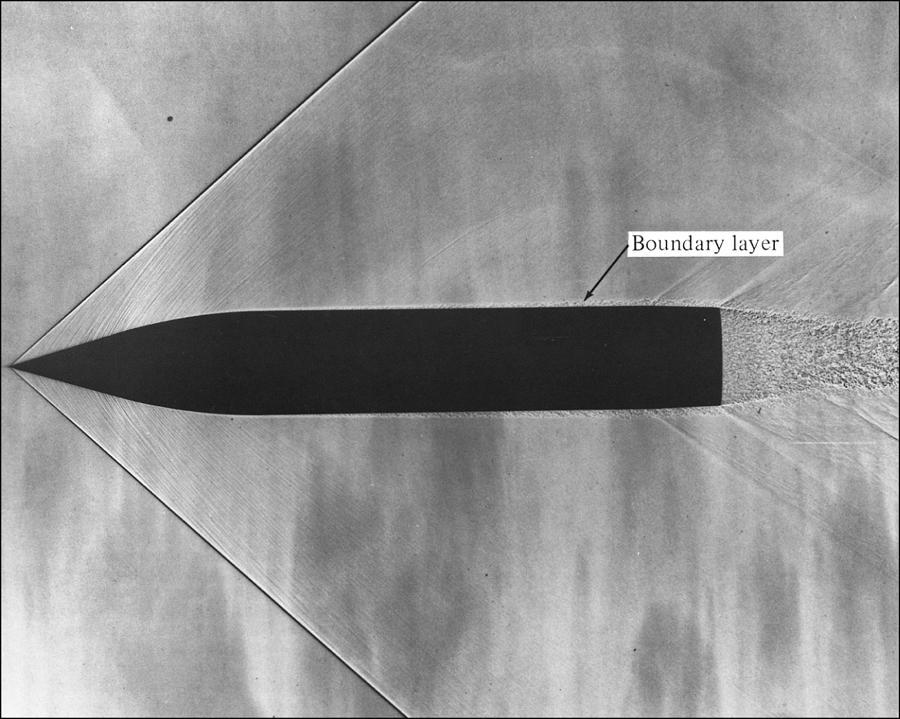
\includegraphics[width=0.9\textwidth]{Motivation/boundary_layer.png}\\
Boundary layer
\end{figure}
\end{column}
\end{columns}
\end{frame}  


% ------------------------------------------------------------
\begin{frame}[t]
\frametitle{Motivation}
\framesubtitle{Initial Mesh Design is Expensive and Time-Consuming}
\begin{columns}[t]
\begin{column}[c]{0.4\textwidth}
\begin{itemize}
  \item Surface mesh must accurately represent geometry
  \item Volume mesh needs sufficient resolution for asymptotic regime
  % Before we accurately know the flow features
  % \item Boundary layer meshes must respect $y^+$ guidelines
  \item Engineers often forced to work by trial and error
  \item Bad in the context of HPC
  \uncover<2>{\item \textcolor{utorange}{We desire an automated computational technology}}
\end{itemize}
\end{column}
\begin{column}[c]{0.6\textwidth}
\vspace{2ex}
\begin{figure}[t]
\centering
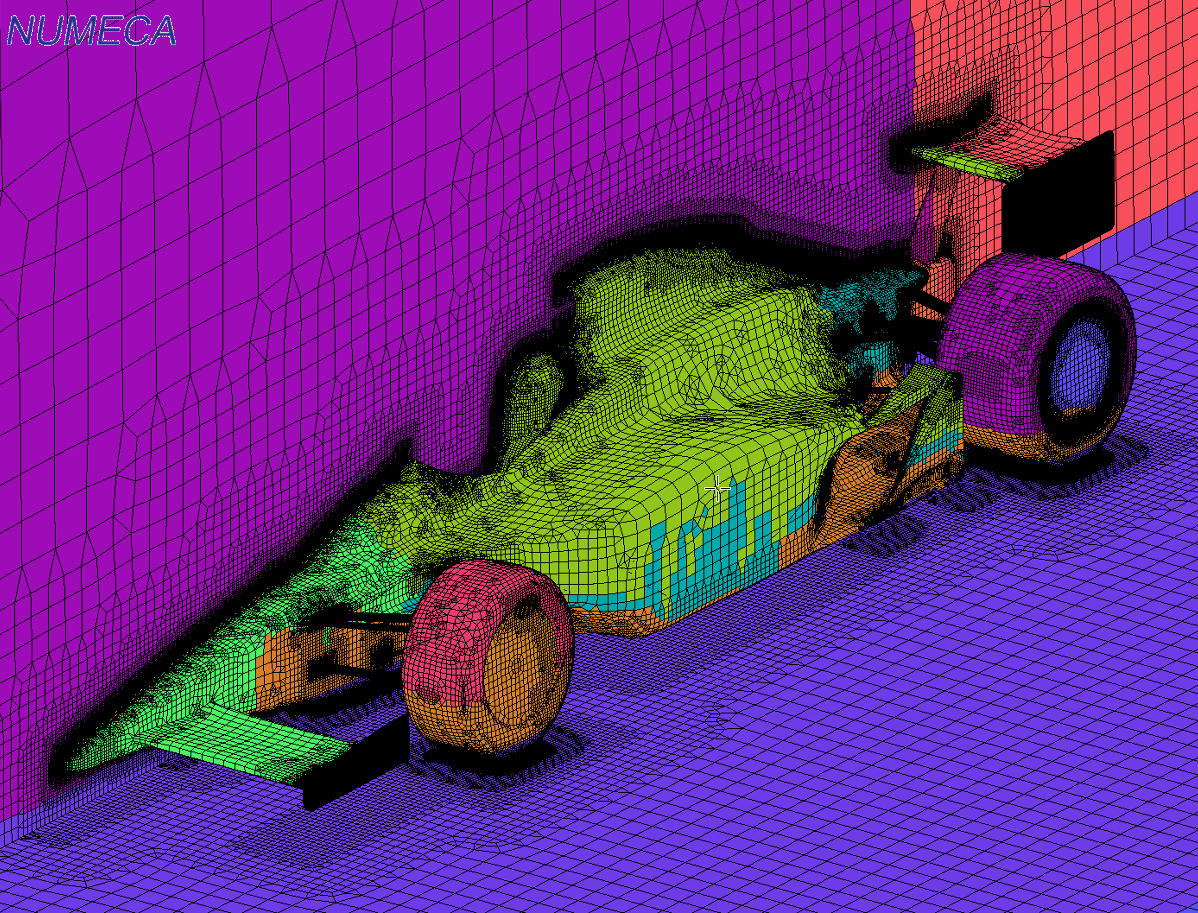
\includegraphics[width=1.0\textwidth]{Motivation/NumecaRaceCar.png}
\\\small{Formula 1 Mesh by Numeca}\\
\end{figure}
\end{column}
\end{columns}
\end{frame}


% ------------------------------------------------------------
\begin{frame}[t]
\frametitle{DPG on Coarse Meshes}
\framesubtitle{Adaptive Solve of the Carter Plate Problem\footfullcite{JesseDissertation} $Re=1000$}
\begin{columns}
\begin{column}{0.49\textwidth}
\begin{figure}
\centering
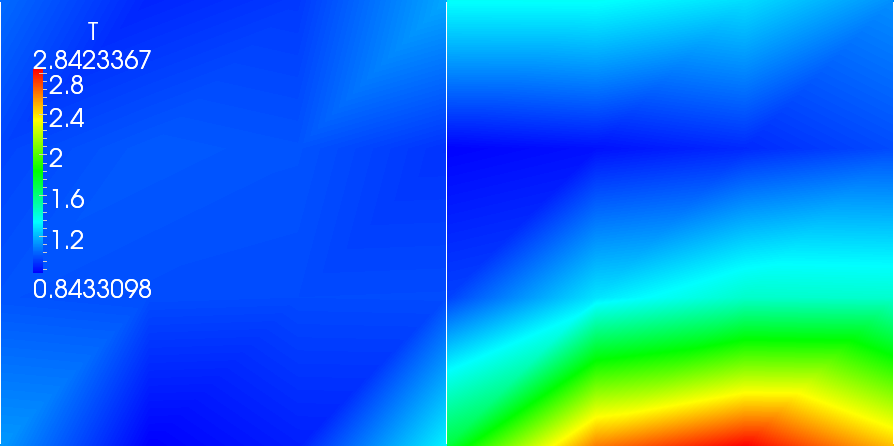
\includegraphics[width=1.0\textwidth]{Motivation/PlateMovie/T0.png}\\
\vspace{-1ex}
{\scriptsize Temperature on Initial Mesh}\\
\vspace{1ex}
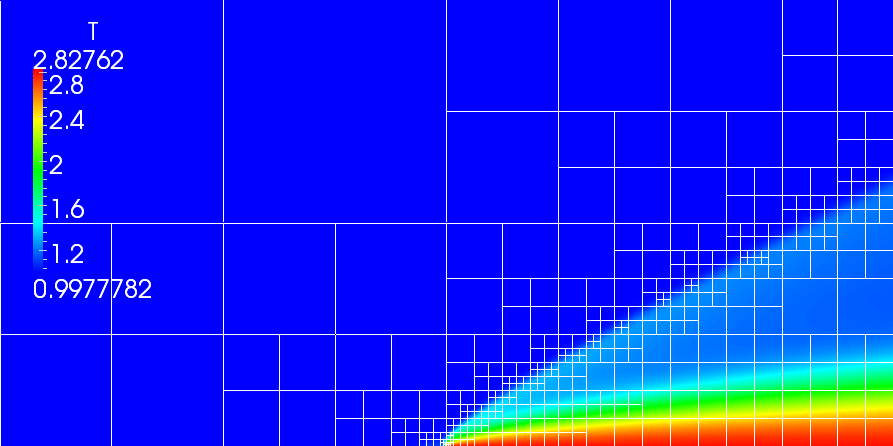
\includegraphics[width=1.0\textwidth]{Motivation/PlateMovie/T8.png}
\vspace{-1ex}
{\scriptsize Temperature after 8 Refinements}
\vspace{1ex}

\end{figure}
\end{column}
\begin{column}{0.49\textwidth}
\begin{figure}
\centering
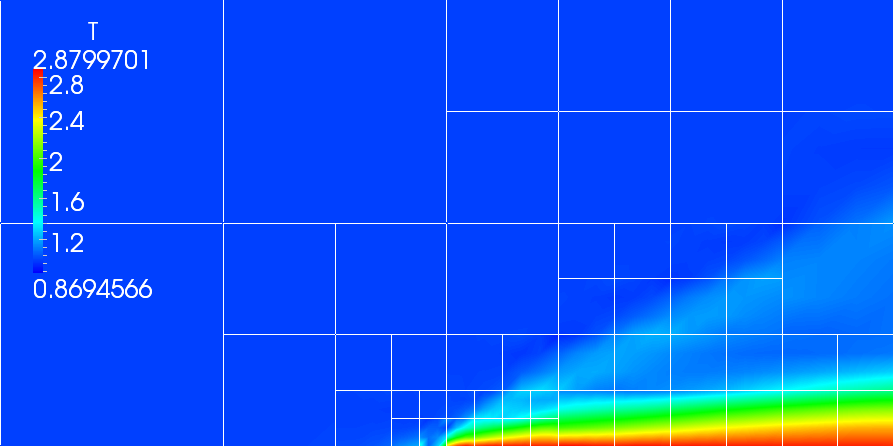
\includegraphics[width=1.0\textwidth]{Motivation/PlateMovie/T4.png}\\
\vspace{-1ex}
{\scriptsize Temperature after 4 Refinements}\\
\vspace{1ex}
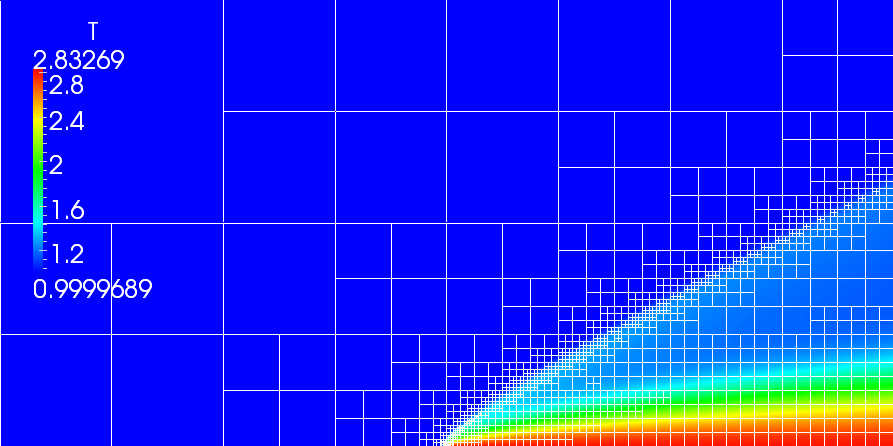
\includegraphics[width=1.0\textwidth]{Motivation/PlateMovie/T11.png}
\vspace{-1ex}
{\scriptsize Temperature after 11 Refinements}
\vspace{1ex}
\end{figure}
\end{column}
\end{columns}
% \foreach \n in {1,...,11}
% {
% \only<\n>
% {
% \begin{figure}[ht]
% \centering
% \begin{subfigure}[c]{0.45\textwidth}
% \centering
% \includegraphics[width=0.99\textwidth]{Motivation/Plate/u\n.png}\\
% \vspace{-1ex}
% {\scriptsize Velocity}\\
% \end{subfigure}
% \begin{subfigure}[c]{0.45\textwidth}
% \centering
% \includegraphics[width=0.99\textwidth]{Motivation/Plate/T\n.png}\\
% \vspace{-1ex}
% {\scriptsize Temperature}\\
% \end{subfigure}
% \begin{subfigure}[c]{0.5\textwidth}
% \centering
% \vspace{2ex}
% \includegraphics[width=0.99\textwidth]{Motivation/Plate/mesh\n.png}\\
% \vspace{-1ex}
% {\scriptsize Mesh \n}\\
% \end{subfigure}
% \end{figure}
% }
% }
\end{frame}

\begin{frame}[t]
\frametitle{Lessons from Other Methods}
\framesubtitle{~~}
\begin{description}
  \item[Streamline Upwind Petrov-Galerkin:] Adaptively changing the test space can produce a method with better stability.
  \item[Discontinuous Galerkin:] Discontinuous basis functions are a legitimate option for finite element methods.
  \item[Hybridized DG:] Mesh interface unknowns can facilitate static condensation -- reducing the number of DOFs in the global solve.
  \item[Least-Squares FEM:] The finite element method is most powerful in a minimum residual context (i.e. as a Ritz method).
  \item[Space-Time FEM:] Highly adaptive methods should have adaptive time integration. 
  Superior framework for problems with moving boundaries.
  Requires a method that is both temporally and spatially stable.
  % \item[Mixed FEM:] A first order formulation gives more flexibility.
\end{description}
% SUPG - changing your test space can produce better stability.

% DG - Discontinuous basis functions are a legitimate option in the finite element framework.

% HDG - Mesh interface unknowns can facilitate static condensation -- reducing the number of DOFs in the global solve.

% Least Squares

% Space-Time FEM - 
%   \item Satisfies geometric conservation laws\footnotemark
%   \item Tezduyar \etal\footnotemark developed a Galerkin/least-squares method for moving boundaries
\end{frame}

%   /$$       /$$   /$$           /$$$$$$$                       /$$                        
%  | $$      |__/  | $$          | $$__  $$                     |__/                        
%  | $$       /$$ /$$$$$$        | $$  \ $$  /$$$$$$  /$$    /$$ /$$  /$$$$$$  /$$  /$$  /$$
%  | $$      | $$|_  $$_/        | $$$$$$$/ /$$__  $$|  $$  /$$/| $$ /$$__  $$| $$ | $$ | $$
%  | $$      | $$  | $$          | $$__  $$| $$$$$$$$ \  $$/$$/ | $$| $$$$$$$$| $$ | $$ | $$
%  | $$      | $$  | $$ /$$      | $$  \ $$| $$_____/  \  $$$/  | $$| $$_____/| $$ | $$ | $$
%  | $$$$$$$$| $$  |  $$$$/      | $$  | $$|  $$$$$$$   \  $/   | $$|  $$$$$$$|  $$$$$/$$$$/
%  |________/|__/   \___/        |__/  |__/ \_______/    \_/    |__/ \_______/ \_____/\___/ 
%                                                                                           
%                                                                                           
%        
% \subsection{Literature Review}
% % ------------------------------------------------------------
% \begin{frame}[t]
% \frametitle{Stabilized Finite Elements for CFD}
% \framesubtitle{Streamline Upwind Petrov-Galerkin}
% \begin{columns}[c]
% \begin{column}{.65\textwidth}
% \begin{itemize}
%   \item First successful finite element method for CFD\footnotemark
%   \item Residual based stabilization preserves consistency
%   \item Upwind biasing of test functions
%   \item Higher order generalizations possible
%   \item Optimal $H_0^1$ approximation in 1D
%   \item Gave rise to the field of stabilized finite elements
%   \item Major contributors include Hughes, Franca, Johnson, Codina, Tezduyar, and many others
%   \item Variational multiscale may be considered the spiritual successor to SUPG\footnotemark
% \end{itemize}
% \end{column}
% \footnotetext[2]{\fullcite{SUPG}}
% \footnotetext[3]{\fullcite{VMS}}
% \begin{column}{.35\textwidth}
% \begin{figure}[t]
% \centering
% 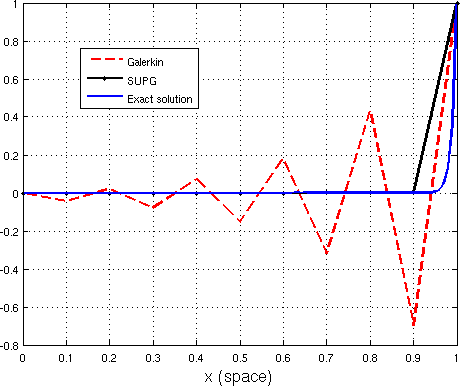
\includegraphics[width=1.0\textwidth]{Motivation/SUPG.png}
% \\\small{$H_0^1$ Projection}\\
% \end{figure}
% \end{column}
% \end{columns}
% \end{frame}


% % ------------------------------------------------------------
% \begin{frame}[t]
% \frametitle{Streamline Upwind Petrov-Galerkin}
% \framesubtitle{Two Equivalent Views on Stabilization}
% Convection-diffusion can be written as
% $$
% Lu=(L_{adv}+L_{diff})u=f\,.
% $$\\
% % Two equivalent views on stabilization.
% \vspace{-3ex}
% \begin{columns}[t]
% \begin{column}{.65\textwidth}
% \begin{block}{Residual Based Stabilization}
% \[
% b_{SUPG}(u,v)=l_{SUPG}(v)
% \]
% where
% \begin{align*}
%   b_{SUPG}(u,v)&=b(u,v)
%   +\sum_K\int_K\tau(L_{adv}v)(Lu-f)\\
%   l_{SUPG}(v)&=l(v)+\sum_K\int_K\tau(L_{adv}v)f\,,
% \end{align*}
% $\tau$ is the SUPG stabilization parameter.
% \end{block}
% \end{column}
% \begin{column}{.33\textwidth}
% \begin{block}{Test Space Modification}
% \[
% b(u,\tilde v)=l(\tilde v)
% \]
% where
% \[
% \tilde v = v+\tau L_{adv}v\,.
% \]
% 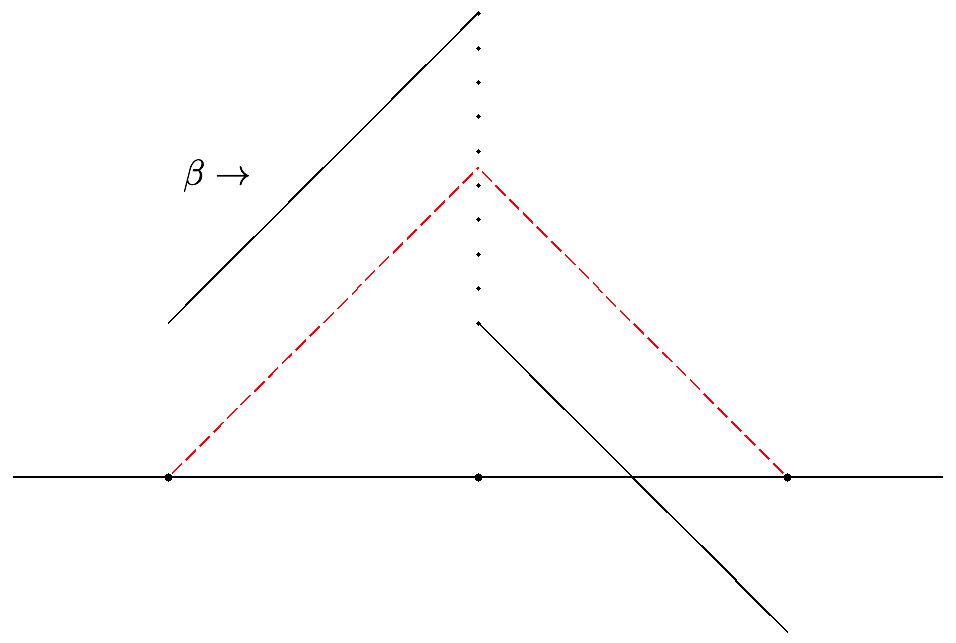
\includegraphics[width=1.0\textwidth]{Motivation/SUPGtest.png}
% \end{block}
% \end{column}
% \end{columns}
% \medskip
% \end{frame}


% % ------------------------------------------------------------
% \begin{frame}[t]
% \frametitle{Stabilized Finite Elements for CFD}
% \framesubtitle{Discontinuous Galerkin}
% \begin{itemize}
%   \item Combines elements of finite volumes and finite elements
%   \item First proposed for neutron transport\footfullcite{ReedHillDG}
%   \item Early contributors include Babu\v{s}ka, Lions, Nitsche, and Zl\'{a}mal
%   \item Develoment for CFD by Cockburn and Shu\footfullcite{CockburnShuDG}
%   \item Development for elliptic problems given by Arnold, Brezzi, Cockburn, and Marini\footfullcite{ArnoldDG}
%   % \item Rigorous mathematical foundation of finite elements
%   \item Nonconforming basis, locally conservative
%   \item Naturally high order, but may require additional stabilization
%   % \item Simple to parallelize
%   \item Other notable contributors include Peraire, Persson, Karniadakis \dots
% \end{itemize}
% \end{frame}


% % ------------------------------------------------------------
% \begin{frame}[t]
% \frametitle{Stabilized Finite Elements for CFD}
% \framesubtitle{Discontinuous Galerkin}
% Consider 1D convection equation
% \[
% \pd{\beta(x)u}{x}=f,\quad u(0)=u_0\,.
% \]
% Multiply by test function and integrate by parts over each element $K=[x_K,x_{x+1}]$
% \[
% -\int_K\beta(x)u\pd{v}{x}+\beta uv|_{x_K}^{x_{K+1}}=\int_K fv\,.
% \]
% Apply upwind flux
% \[
% -\int_K\beta(x)u\pd{v}{x}+\beta(x_{K+1})u(x_{K+1}^-)v(x_{K+1}^-)-\beta(x_K)u(x_K^-)v(x_K^+)=\int_K fv\,.
% \]
% Hybridized DG (HDG) method introduces trace unknowns which facilitates static condensation, reducing interface unknowns\footfullcite{HDG}.
% \end{frame}

% % ------------------------------------------------------------
% \begin{frame}[t]
% \frametitle{Space-Time Finite Element Methods}
% \framesubtitle{Treat Time as Another Dimension to be Discretized}
% Space-time methods treat time as just another dimension to be discretized.
% \begin{columns}[c]
% \begin{column}{.7\textwidth}
% \begin{itemize}
%   \item Early contributors include Kaczkowski and Oden 
%   \item Satisfies geometric conservation laws\footnotemark
%   \item Tezduyar \etal\footnotemark developed a Galerkin/least-squares method for moving boundaries
%   % deforming-spatial-domain/space-time procedure 
%   % with Galerkin/least-squares to handle moving domains with incompressible and compressible flow
%   \item Van der Vegt and Van der Ven developed a popular space-time DG method\footnotemark
%   \item {\"U}ng{\"o}r's tent-pitcher algorithm\footnotemark decouples space-time elements
% \end{itemize}
% \end{column}
% \footnotetext[8]{\fullcite{GCL}}
% \footnotetext[9]{\fullcite{Tezduyar1992}}
% \footnotetext[10]{\fullcite{vanderVegtEuler}}
% \footnotetext[11]{\fullcite{TentPitcher}}
% \begin{column}{.3\textwidth}
% 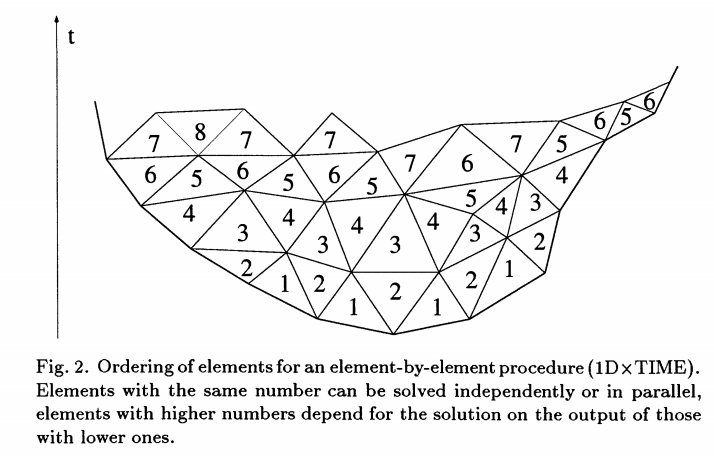
\includegraphics[width=1.0\textwidth]{Motivation/TentPitcher.png}
% \end{column}
% \end{columns}
% \end{frame}



%   /$$$$$$$  /$$$$$$$   /$$$$$$         /$$$$$$                                            /$$                        
%  | $$__  $$| $$__  $$ /$$__  $$       /$$__  $$                                          |__/                        
%  | $$  \ $$| $$  \ $$| $$  \__/      | $$  \ $$ /$$    /$$  /$$$$$$   /$$$$$$  /$$    /$$ /$$  /$$$$$$  /$$  /$$  /$$
%  | $$  | $$| $$$$$$$/| $$ /$$$$      | $$  | $$|  $$  /$$/ /$$__  $$ /$$__  $$|  $$  /$$/| $$ /$$__  $$| $$ | $$ | $$
%  | $$  | $$| $$____/ | $$|_  $$      | $$  | $$ \  $$/$$/ | $$$$$$$$| $$  \__/ \  $$/$$/ | $$| $$$$$$$$| $$ | $$ | $$
%  | $$  | $$| $$      | $$  \ $$      | $$  | $$  \  $$$/  | $$_____/| $$        \  $$$/  | $$| $$_____/| $$ | $$ | $$
%  | $$$$$$$/| $$      |  $$$$$$/      |  $$$$$$/   \  $/   |  $$$$$$$| $$         \  $/   | $$|  $$$$$$$|  $$$$$/$$$$/
%  |_______/ |__/       \______/        \______/     \_/     \_______/|__/          \_/    |__/ \_______/ \_____/\___/ 
%                                                                                                                      
%                                                                                                                      
% 
\section{DPG: A Framework for Computational Mechanics}
% ------------------------------------------------------------
\begin{frame}[t]
\frametitle{Overview of DPG}
\framesubtitle{DPG is a Minimum Residual Method}
Find $u\in U$ such that
\[
b(u,v)=l(v)\quad\forall v\in V
\]
with operator $B:U\rightarrow V'$ defined by $b(u,v)=\LRa{Bu,v}_{V'\times V}$.

This gives the operator equation 
\[
Bu=l\quad\in V'\,.
\]
We wish to minimize the residual $Bu-l\in V'$:
\[
u_h=\argmin_{w_h\in U_h}\frac{1}{2}\norm{Bw_h-l}^2_{V'}\,.
\]
Dual norms are not computationally tractable. 
Inverse Riesz map moves the residual to a more accessible space:
\[
u_h=\argmin_{w_h\in U_h}\frac{1}{2}\norm{R_V^{-1}(Bw_h-l)}^2_{V}\,.
\]
\end{frame}


% ------------------------------------------------------------
\begin{frame}[t]
\frametitle{Overview of DPG}
\framesubtitle{Petrov-Galerkin with Optimal Test Functions}
% \framesubtitle{Optimal Petrov-Galerkin Methods}
Taking the G\^ateaux derivative to be zero in all directions $\delta u \in
U_h$ gives,
\[
\left(R_V^{-1}(Bu_h-l),R_V^{-1}B\delta u\right)_V = 0, \quad \forall \delta u \in U,
\]
which by definition of the Riesz map is equivalent to 
\begin{equation*}
\LRa{Bu_h-l,R_V^{-1}B\delta u_h}=0\quad\forall\delta u_h\in U_h\,,
\end{equation*}
with optimal test functions $v_{\delta u_h}\coloneqq R_V^{-1}B\delta u_h$ for each trial function $\delta u_h$.
\begin{block}{Resulting Petrov-Galerkin System}
This gives a simple bilinear form
\begin{equation*}
b(u_h,v_{\delta u_h})=l(v_{\delta u_h}),
\end{equation*}
with $v_{\delta u_h}\in V$ that solves the auxiliary problem
\begin{equation*}
\LRp{v_{\delta u_h},\delta v}_V=\LRa{R_Vv_{\delta u_h},\delta v}
=\LRa{B\delta u_h,\delta v}=b(\delta u_h,\delta v)\quad\forall\delta v\in V.
\end{equation*}
\end{block}
\end{frame}

% ------------------------------------------------------------
\begin{frame}[t]
\frametitle{Overview of DPG}
\framesubtitle{Mixed Formulation}
Identifying the error representation function:
\[
\psi:=R_V^{-1}(Bu_h-l)
\] 
allows us to develop an alternative interpretation of DPG.
\begin{block}{DPG as a Mixed Problem}
Find $\psi\in V$, $u_h\in U_h$ such that
\begin{equation*}
\begin{aligned}
\LRp{\psi,\delta v}_V-b(u_h,\delta v)&=-l(\delta v) \quad&\forall&\delta v&\in V\\
b(\delta u_h,\psi)&=0 \quad&\forall&\delta u_h&\in U_h
\end{aligned}
\end{equation*}
\end{block}
In this unconventional saddle-saint problem, the approximate solution $u_h$ comes from a finite-dimensional
trial space and plays the role of the Lagrange multiplier for the error representation function
\end{frame}


% ------------------------------------------------------------
\begin{frame}[t]
\frametitle{Overview of DPG}
\framesubtitle{DPG is the Most Stable Petrov-Galerkin Method}
Babu\v{s}ka's theorem guarantees that \emph{discrete stability and approximability imply convergence}.
If bilinear form $b(u,v)$, with $M:=\norm{b}$ satisfies the discrete inf-sup condition 
with constant $\gamma_h$,
\[
\sup_{v_h\in V_h}\frac{|b(u,v)|}{\norm{v_h}_V}\geq\gamma_h\norm{u_h}_U\,,
\]
then the Galerkin error satisfies the bound
\[
\norm{u_h-u}_U\leq\frac{M}{\gamma_h}\inf_{w_h\in U_h}\norm{w_h-u}_U\,.
\]
Optimal test function realize the supremum guaranteeing that $\gamma_h\geq\gamma$.\\
\begin{block}{Energy Norm}
If we use the energy norm, $\norm{u}_E:=\norm{Bu}_{V'}$ in the error estimate, then $M=\gamma=1$.
Babu\v{s}ka's theorem
implies that the minimum residual method is the most stable Petrov-Galerkin method (assuming exact optimal test functions).
\end{block}
\end{frame}


% ------------------------------------------------------------
% \begin{frame}[t]
% \frametitle{Overview of DPG}
% \framesubtitle{Optimal Test Functions}
% Plots of Poisson, Convection, Convection-Diffusion, etc
% \end{frame}


% ------------------------------------------------------------
\begin{frame}[t]
\frametitle{Overview of DPG}
% \footfullcite{DPGOverview}}
\framesubtitle{Other Features}
\begin{block}{Discontinuous Petrov-Galerkin}
\begin{itemize}
  \item Continuous test space produces global solve for optimal test functions
  \item Discontinuous test space results in an embarrassingly parallel solve
\end{itemize}
\end{block}
\begin{block}{Hermitian Positive Definite Stiffness Matrix}
Property of all minimum residual methods
\[
b(u_h,v_{\delta u_h})=\LRp{v_{u_h},v_{\delta u_h}}_V=\overline{\LRp{v_{\delta u_h},v_{u_h}}_V}=\overline{b(\delta u_h,v_{u_h})}
\]
\end{block}
\begin{block}{Error Representation Function}
Energy norm of Galerkin error (residual) can be computed without exact solution
\[
\norm{u_h-u}_E=\norm{B(u_h-u)}_{V'}=\norm{Bu_h-l}_{V'}=\norm{R_V^{-1}(Bu_h-l)}_V
\]
\end{block}
\end{frame}


% ------------------------------------------------------------
\begin{frame}[t]
\frametitle{Overview of DPG}
\framesubtitle{High Performance Computing}
\begin{columns}[c]
\begin{column}{.5\textwidth}
Eliminates human intervention
\medskip

\begin{itemize}
  \item Stability
  \item Robustness
  \item Adaptivity
  \item Automaticity
  \item Compute intensive
  \item Embarrassingly parallel local solves
  \item Factorization recyclable
  \item Low communication
  \item SPD stiffness matrix
  \item Multiphysics
\end{itemize}

% Issues to be solved
% \begin{itemize}
%   \item Iterative solvers
% \end{itemize}
\end{column}
\begin{column}{.5\textwidth}
\vspace{-3ex}
\begin{figure}[t]
\centering
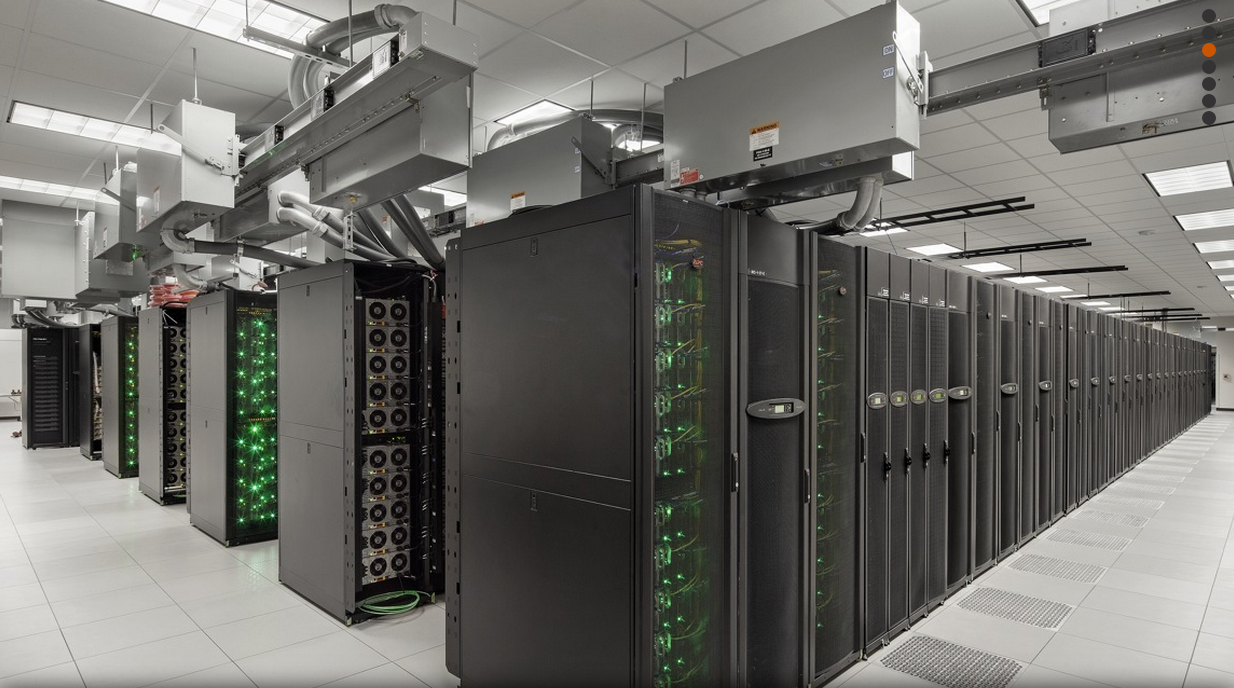
\includegraphics[width=0.9\textwidth]{Motivation/Stampede.png}
\\\small{Stampede Supercomputer at TACC}\\
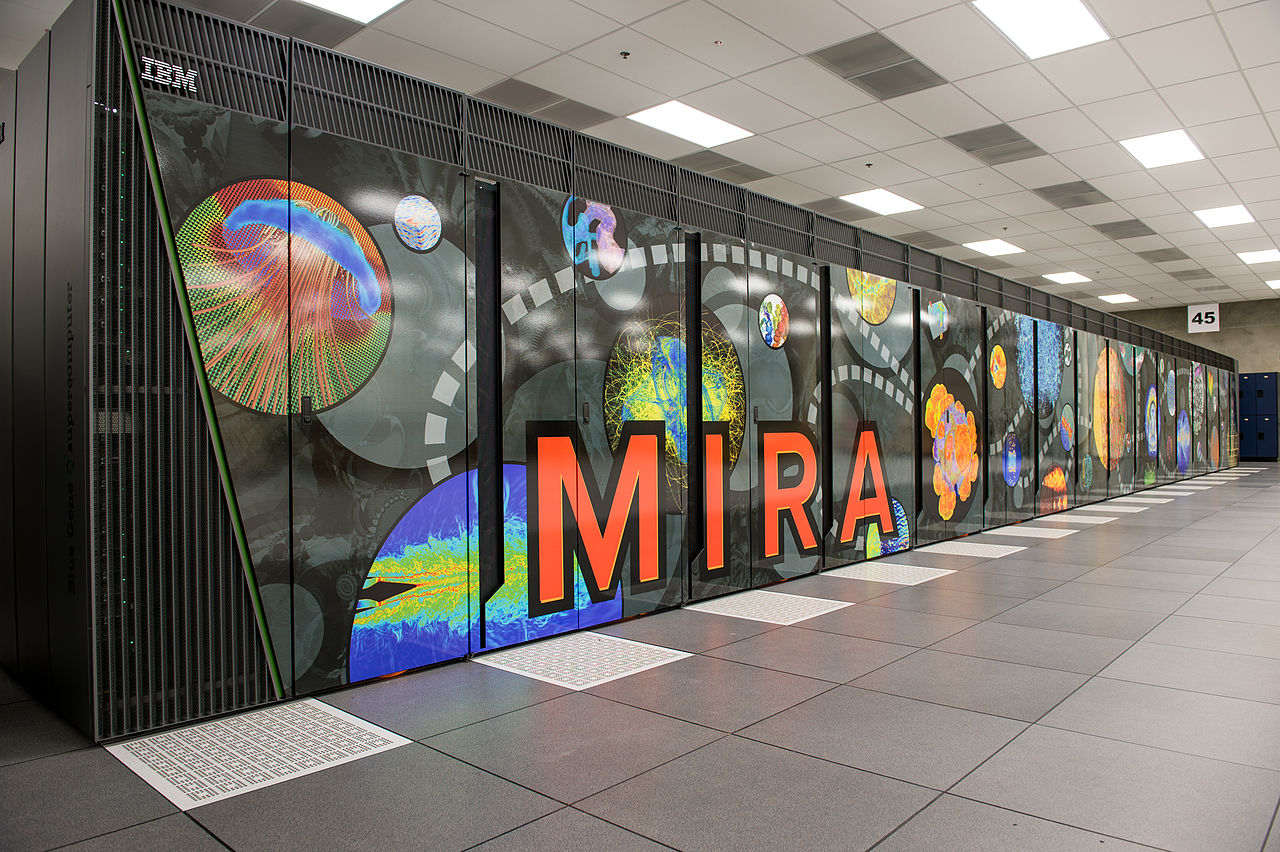
\includegraphics[width=0.9\textwidth]{Motivation/Mira.png}
\\\small{Mira Supercomputer at Argonne}\\
\end{figure}
\end{column}
\end{columns}

\end{frame}






%   /$$        /$$$$$$ 
%  | $$       /$$__  $$
%  | $$      | $$  \__/
%  | $$      | $$      
%  | $$      | $$      
%  | $$      | $$    $$
%  | $$$$$$$$|  $$$$$$/
%  |________/ \______/ 
%                      
%                      
%      
\section{Local Conservation}
%===============================================================================
% NEW SLIDE
%===============================================================================
\begin{frame}
\frametitle{Locally Conservative DPG}
\framesubtitle{DPG for Convection-Diffusion}
Start with the strong-form PDE.
\[
\nabla\cdot(\bfbeta u)-\epsilon\Delta u = g
\]
Rewrite as a system of first-order equations.
\begin{align*}
\frac{1}{\epsilon}\bfsigma-\nabla u&=\boldsymbol0\\
\nabla\cdot(\bfbeta u-\bfsigma)&=g
\end{align*}
Multiply by test functions and integrate by parts over each element, $K$.
\begin{align*}
\frac{1}{\epsilon}(\bfsigma,\bftau)_K+(u,\nabla\cdot\bftau)_K
-\LRa{u,\tau_n}_{\partial K}&=0\\
-(\bfbeta u-\bfsigma,\nabla v)_K+\LRa{(\bfbeta
u-\bfsigma)\cdot\mathbf{n},v}_{\partial K}&=(g,v)_K
\end{align*}
Use the ultraweak (DPG) formulation to obtain bilinear form $b(u,v)=l(v)$.
\begin{align*}
\frac{1}{\epsilon}(\bfsigma,\bftau)_K
&+(u,\nabla\cdot\bftau)_K-\LRa{\hat u,\tau_n}_{\partial K}\\
&-(\bfbeta u-\bfsigma,\nabla v)_K+\LRa{\hat t,v}_{\partial K}
=(g,v)_K
\end{align*}
\end{frame}


%    /$$$$$$                                                                           /$$     /$$                     
%   /$$__  $$                                                                         | $$    |__/                     
%  | $$  \__/  /$$$$$$  /$$$$$$$   /$$$$$$$  /$$$$$$   /$$$$$$  /$$    /$$  /$$$$$$  /$$$$$$   /$$ /$$    /$$  /$$$$$$ 
%  | $$       /$$__  $$| $$__  $$ /$$_____/ /$$__  $$ /$$__  $$|  $$  /$$/ |____  $$|_  $$_/  | $$|  $$  /$$/ /$$__  $$
%  | $$      | $$  \ $$| $$  \ $$|  $$$$$$ | $$$$$$$$| $$  \__/ \  $$/$$/   /$$$$$$$  | $$    | $$ \  $$/$$/ | $$$$$$$$
%  | $$    $$| $$  | $$| $$  | $$ \____  $$| $$_____/| $$        \  $$$/   /$$__  $$  | $$ /$$| $$  \  $$$/  | $$_____/
%  |  $$$$$$/|  $$$$$$/| $$  | $$ /$$$$$$$/|  $$$$$$$| $$         \  $/   |  $$$$$$$  |  $$$$/| $$   \  $/   |  $$$$$$$
%   \______/  \______/ |__/  |__/|_______/  \_______/|__/          \_/     \_______/   \___/  |__/    \_/     \_______/
%                                                                                                                      
%                                                                                                                      
%     
%===============================================================================
% NEW SLIDE
%===============================================================================
\begin{frame}
\frametitle{Locally Conservative DPG}
\framesubtitle{Local Conservation for Convection-Diffusion}
The local conservation law in convection diffusion is
\[
\int_{\partial K}\hat t=\int_K g\,,
\]
which is equivalent to having $\mathbf{v}_K:=\{v,\bftau\}=\{1_K,\boldsymbol0\}$ in the test space.
In general, this is not satisfied by the optimal test functions.
Following Moro et al\footfullcite{MoroNguyenPeraire11} (also
Chang and Nelson\footfullcite{ChangNelson1997}), we
can enforce this condition with Lagrange multipliers:
\begin{align*}
L(u_h,\bflambda) = \frac{1}{2}\norm{R_V^{-1}(Bu_h-l)}_V^2
-\sum_K\lambda_K\underbrace{\langle Bu_h-l,\mathbf{v}_K\rangle}_
{\langle\hat t, 1_K\rangle_{\partial K}-\langle g,1_K\rangle_K}\,,
\end{align*}
where $\bflambda=\{\lambda_1,\cdots,\lambda_N\}$.
\end{frame}


%===============================================================================
% NEW SLIDE
%===============================================================================
\begin{frame}
\frametitle{Locally Conservative DPG}
\framesubtitle{Locally Conservative Saddle Point System}
Finding the critical points of $L(u,\bflambda)$, we get the following
equations.
\begin{block}{Locally Conservative Saddle Point System}
\begin{align*}
\frac{\partial L(u_h,\bflambda)}{\partial u_h}&=b(u_h,R_V^{-1}B\delta u_h)
-l(R_V^{-1}B\delta u_h)\\
&{\color{red}-\sum_K\lambda_K b(\delta
u_h,\mathbf{v}_K)}=0\quad\forall\delta u_h\in U_h
\end{align*}
\[
\frac{\partial
L(u_h,\bflambda)}{\partial\lambda_K}=-b(u_h,\mathbf{v}_K)+l(\mathbf{v}_K)=0\quad\forall
K
\]
\end{block}
A few consequences:
\begin{itemize}
\item We've turned our minimization problem into a saddle point problem.
% \item New $\lambda_K$ DOFs can be statically condensed out.
\item Only need to find the optimal test function in the orthogonal complement
of constants. % Backup slide
\end{itemize}
\end{frame}


%===============================================================================
% NEW SLIDE
%===============================================================================
\begin{frame}
\frametitle{Locally Conservative DPG}
\framesubtitle{Optimal Test Functions}
For each $\mathbf{u}=\{u,\bfsigma,\hat u,\hat t\}\in\mathbf{U}_h$, find
$\mathbf{v}_{\mathbf{u}}=\{v_\mathbf{u},\bftau_\mathbf{u}\}\in\mathbf{V}$ such that
\[
(\mathbf{v_u},\mathbf{w})_\mathbf{V}=b(\mathbf{u},\mathbf{w})\quad\forall\mathbf{w}\in\mathbf{V}
\]
where $\mathbf{V}$ becomes $\mathbf{V}_{p+\Delta p}$ in order to make this
computationally tractable.

We recently developed this modification to the \emph{robust test norm}
\footfullcite{ChanHeuerThanhDemkowicz2012} which behaves better in
the presence of singularities.
\begin{block}{Convection-Diffusion Test Norm}
\begin{minipage}[t][1.2in]{\textwidth}
\begin{align*}
\norm{(v,\bftau)}^2_{\mathbf{V},\Omega_h}&=
\norm{\min\left\{\frac{1}{\sqrt{\epsilon}},\frac{1}{\sqrt{|K|}}\right\}\bftau}^2
+\norm{\nabla\cdot\bftau-\bfbeta\cdot\nabla v}^2\\
&+\norm{\bfbeta\cdot\nabla v}^2+\epsilon\norm{\nabla v}^2
\underbrace{\color{red}{
\begin{minipage}[c][0.3in][c]{0.9in}$
\only<1>{
\hspace{1.5ex}
+\norm{v}^2
}
\only<2>{
+\left(\frac{1}{|K|}\int_Kv\right)^2
}$
\end{minipage}
}}_{\only<1>{\text{No longer necessary}}\only<2>{\text{Scaling term}}}
\end{align*}
\end{minipage}
\end{block}
\end{frame}


%    /$$$$$$    /$$               /$$       /$$ /$$ /$$   /$$              
%   /$$__  $$  | $$              | $$      |__/| $$|__/  | $$              
%  | $$  \__/ /$$$$$$    /$$$$$$ | $$$$$$$  /$$| $$ /$$ /$$$$$$   /$$   /$$
%  |  $$$$$$ |_  $$_/   |____  $$| $$__  $$| $$| $$| $$|_  $$_/  | $$  | $$
%   \____  $$  | $$      /$$$$$$$| $$  \ $$| $$| $$| $$  | $$    | $$  | $$
%   /$$  \ $$  | $$ /$$ /$$__  $$| $$  | $$| $$| $$| $$  | $$ /$$| $$  | $$
%  |  $$$$$$/  |  $$$$/|  $$$$$$$| $$$$$$$/| $$| $$| $$  |  $$$$/|  $$$$$$$
%   \______/    \___/   \_______/|_______/ |__/|__/|__/   \___/   \____  $$
%                                                                 /$$  | $$
%                                                                |  $$$$$$/
%                                                                 \______/ 
%===============================================================================
% NEW SLIDE
%===============================================================================
\begin{frame}
\frametitle{Locally Conservative DPG}
\framesubtitle{Stability and Robustness Analysis}
\begin{itemize}
\item We follow Brezzi's theory for an abstract mixed problem:
\begin{equation*}
\left\{
\begin{array}{lll}
\bfu \in \bfU, p \in Q\\
a(\bfu,\bfw) + c(p,\bfw) & = l(\bfw) & \forall \bfw \in \bfU \\
c(q,\bfu) & = g(q) & \forall q \in Q
\end{array}
\right.
\end{equation*}
where $a,c,l,g$ denote the appropriate
bilinear and linear forms. 
\item $a(\bfu,\bfw)=b(\bfu,R_V^{-1}B\bfw)=(R_V^{-1}B\bfu,R_V^{-1}B\bfw)_V$
\item $c(p,\bfw)=\sum_K\lambda_K\LRa{\hat t,1_K}_{\partial K}$

\item Locally conservative DPG satisfies inf-sup and inf-sup in kernel conditions.

\item Robustness is proved by switching to energy norm in Brezzi analysis.

\item Full details can be found in \emph{Locally Conservative Discontinuous Petrov-Galerkin Finite Elements for Fluid Problems}\footfullcite{EllisLC}.
\end{itemize}
\end{frame}



% %   /$$$$$$$$           /$$           /$$                                    
% %  | $$_____/          |__/          | $$                                    
% %  | $$        /$$$$$$  /$$  /$$$$$$$| $$   /$$  /$$$$$$$  /$$$$$$  /$$$$$$$ 
% %  | $$$$$    /$$__  $$| $$ /$$_____/| $$  /$$/ /$$_____/ /$$__  $$| $$__  $$
% %  | $$__/   | $$  \__/| $$| $$      | $$$$$$/ |  $$$$$$ | $$  \ $$| $$  \ $$
% %  | $$      | $$      | $$| $$      | $$_  $$  \____  $$| $$  | $$| $$  | $$
% %  | $$$$$$$$| $$      | $$|  $$$$$$$| $$ \  $$ /$$$$$$$/|  $$$$$$/| $$  | $$
% %  |________/|__/      |__/ \_______/|__/  \__/|_______/  \______/ |__/  |__/
% %                                                                            
% %                                                                            
% %   
% %===============================================================================
% % NEW SLIDE
% %===============================================================================
% \begin{frame}
% \frametitle{Numerical Experiments}
% \framesubtitle{Eriksson-Johnson Problem}
% On domain $\Omega=[0,1]^2$, with $\beta=(1,0)^T$, $f=0$ and boundary
% conditions
% \[
% \hat t=u_0,\quad\beta_n\le0\,,\quad\quad\hat u=0,\quad\beta_n > 0
% \]
% Separation of variabes gives an analytic solution
% \[
% u(x,y)=C_0+\sum_{n=1}^\infty C_n
% \frac{\exp(r_2(x-1))-\exp(r_1(x-1))}{r_1\exp(-r_2)-r_2\exp(-r_1)}
% \cos(n\pi y)
% \]
% \vspace{-5ex}
% \begin{columns}[b]
% \begin{column}{0.5\textwidth}
% \begin{figure}[t]
% \centering
% 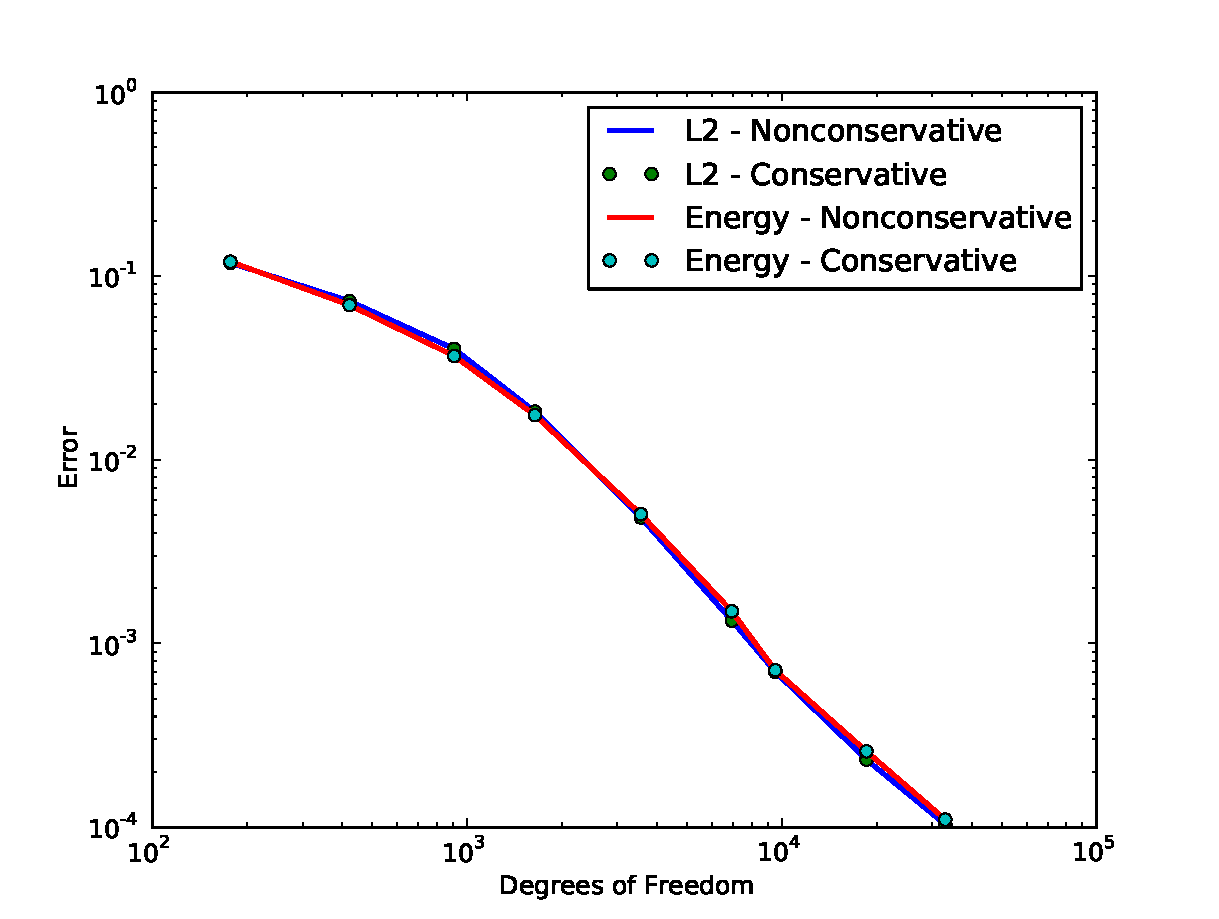
\includegraphics[width=0.9\textwidth]{Erickson/modifiedError.pdf}

% \end{figure}
% \end{column}
% \begin{column}{0.5\textwidth}
% \begin{figure}[t]
% \centering
% 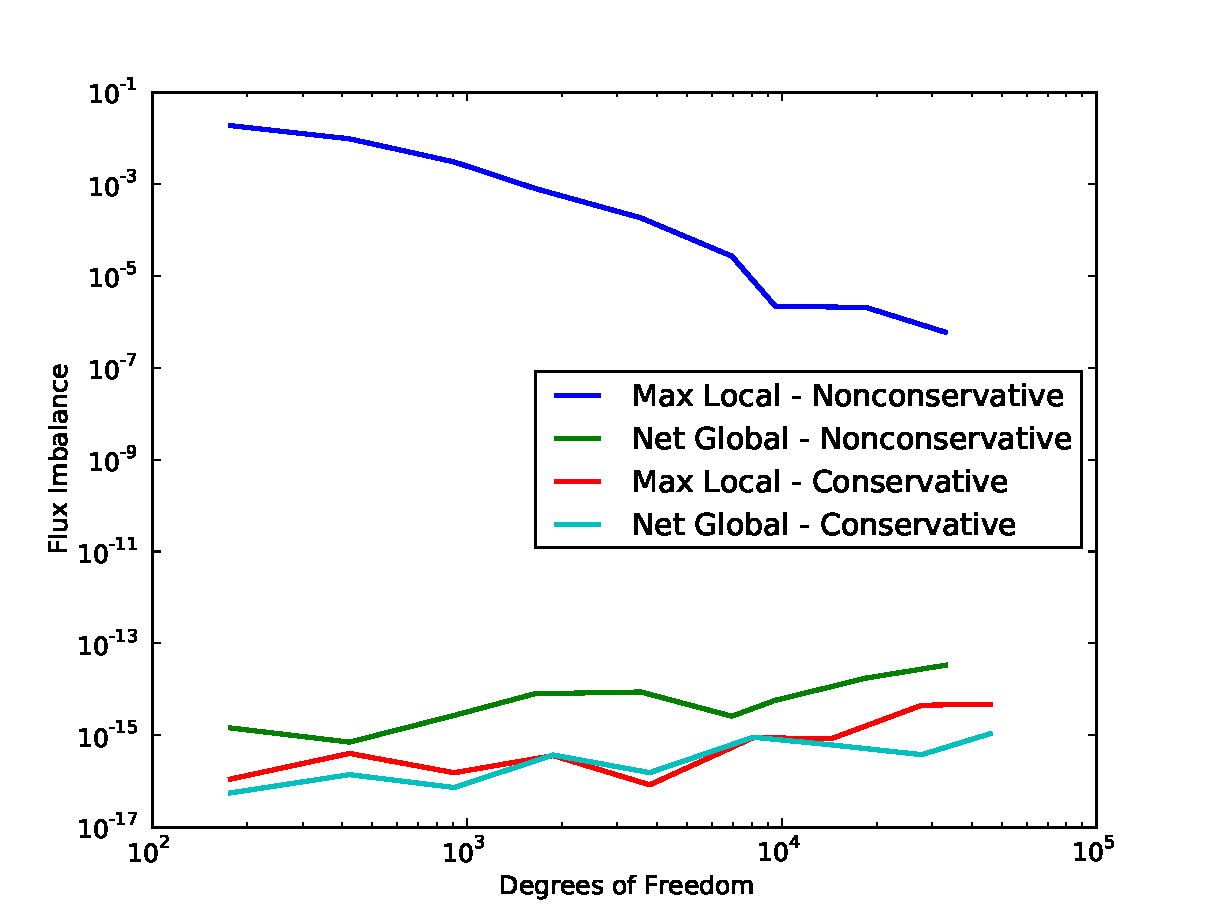
\includegraphics[width=0.9\textwidth]{Erickson/modifiedFlux.pdf}

% \end{figure}
% \end{column}
% \end{columns}
% \end{frame}


%    /$$$$$$    /$$               /$$                          
%   /$$__  $$  | $$              | $$                          
%  | $$  \__/ /$$$$$$    /$$$$$$ | $$   /$$  /$$$$$$   /$$$$$$$
%  |  $$$$$$ |_  $$_/   /$$__  $$| $$  /$$/ /$$__  $$ /$$_____/
%   \____  $$  | $$    | $$  \ $$| $$$$$$/ | $$$$$$$$|  $$$$$$ 
%   /$$  \ $$  | $$ /$$| $$  | $$| $$_  $$ | $$_____/ \____  $$
%  |  $$$$$$/  |  $$$$/|  $$$$$$/| $$ \  $$|  $$$$$$$ /$$$$$$$/
%   \______/    \___/   \______/ |__/  \__/ \_______/|_______/ 
%                                                              
%                                                              
%   
%===============================================================================
% NEW SLIDE
%===============================================================================
\begin{frame}
\frametitle{Numerical Experiments}
\framesubtitle{Stokes Flow Around a Cylinder}
\only<1>{
\centering
Horizontal Velocity
\vspace{-1ex}
}
\only<2>{
\centering
Percent Mass Loss at $x=[-1, -0.95, 0, 0.95, 3]$
\vspace{-5ex}
}
\begin{columns}
\begin{column}{0.49\textwidth}
\only<1>{
\begin{figure}
\centering
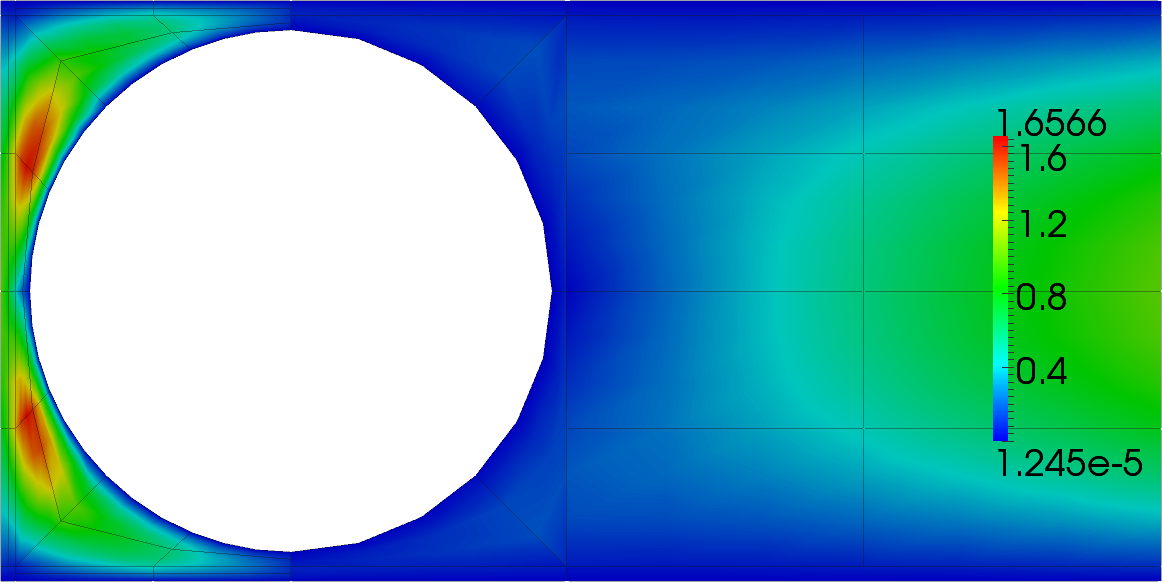
\includegraphics[width=0.95\textwidth]{StokesCylinder/umag9_NC1.png}\\
\vspace{-1ex}

{\scriptsize 1 Refinement}\\
\vspace{1ex}
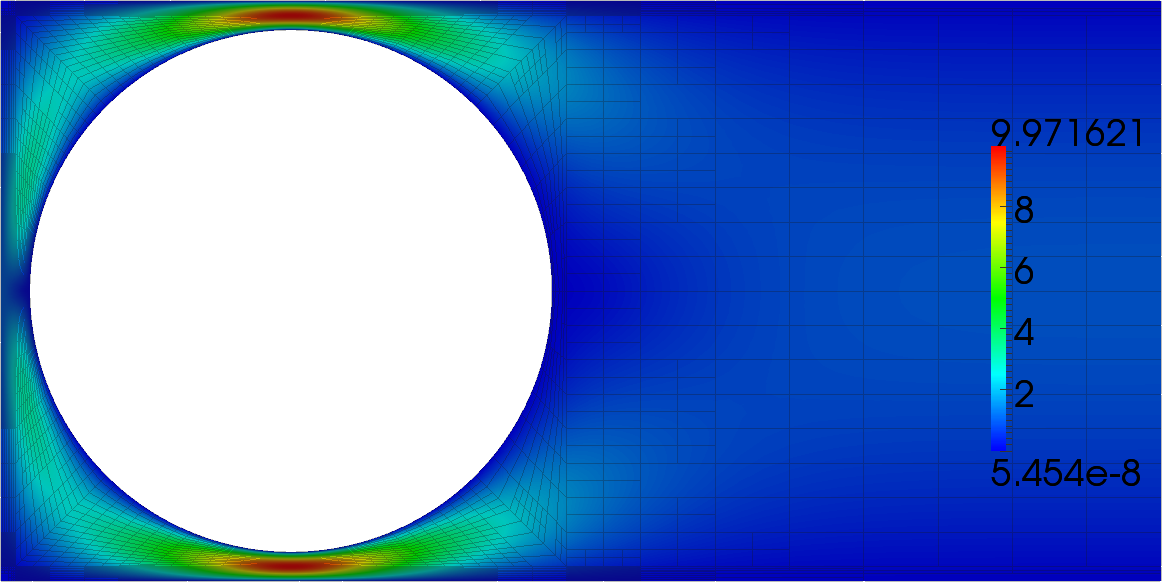
\includegraphics[width=0.95\textwidth]{StokesCylinder/umag9_NC6.png}
\vspace{-1ex}

{\scriptsize 6 Refinements}
% \vspace{1ex}

Nonconservative
\end{figure}
\end{column}
\begin{column}{0.49\textwidth}
\begin{figure}
\centering
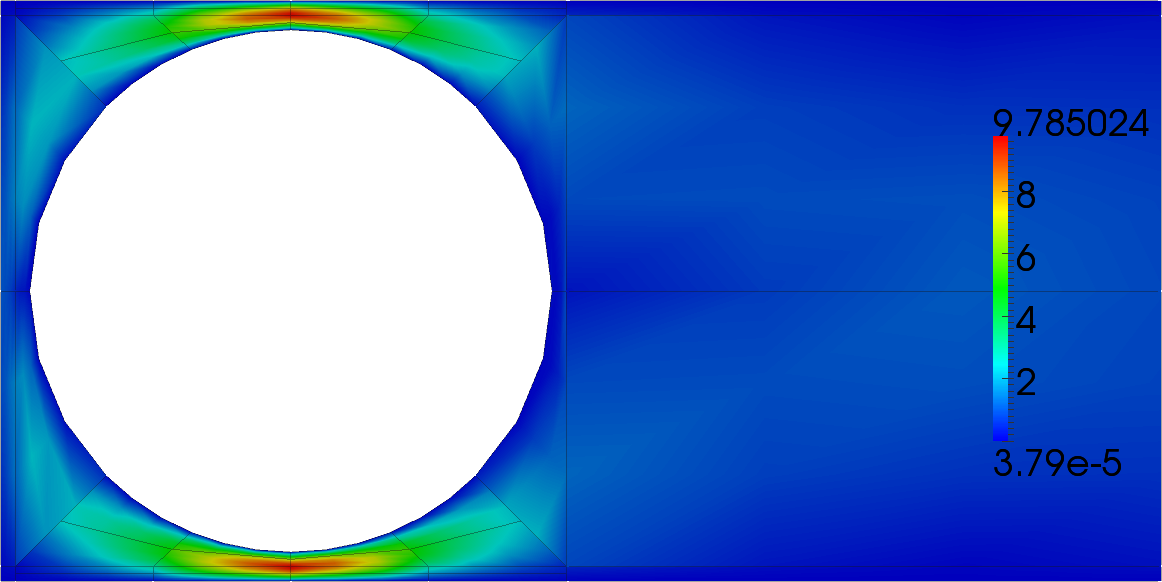
\includegraphics[width=0.95\textwidth]{StokesCylinder/umag9_C1.png}\\
\vspace{-1ex}

{\scriptsize 1 Refinement}\\
\vspace{1ex}
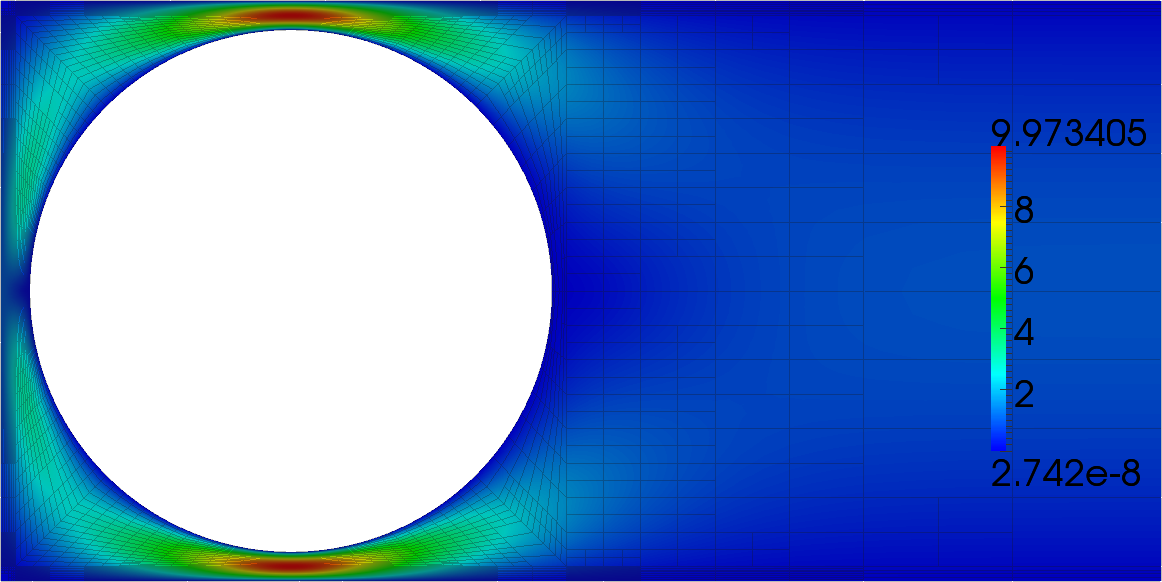
\includegraphics[width=0.95\textwidth]{StokesCylinder/umag9_C6.png}
\vspace{-1ex}

{\scriptsize 6 Refinements}
% \vspace{1ex}

Conservative
\end{figure}
}
\only<2>{
\begin{figure}[t]
\centering
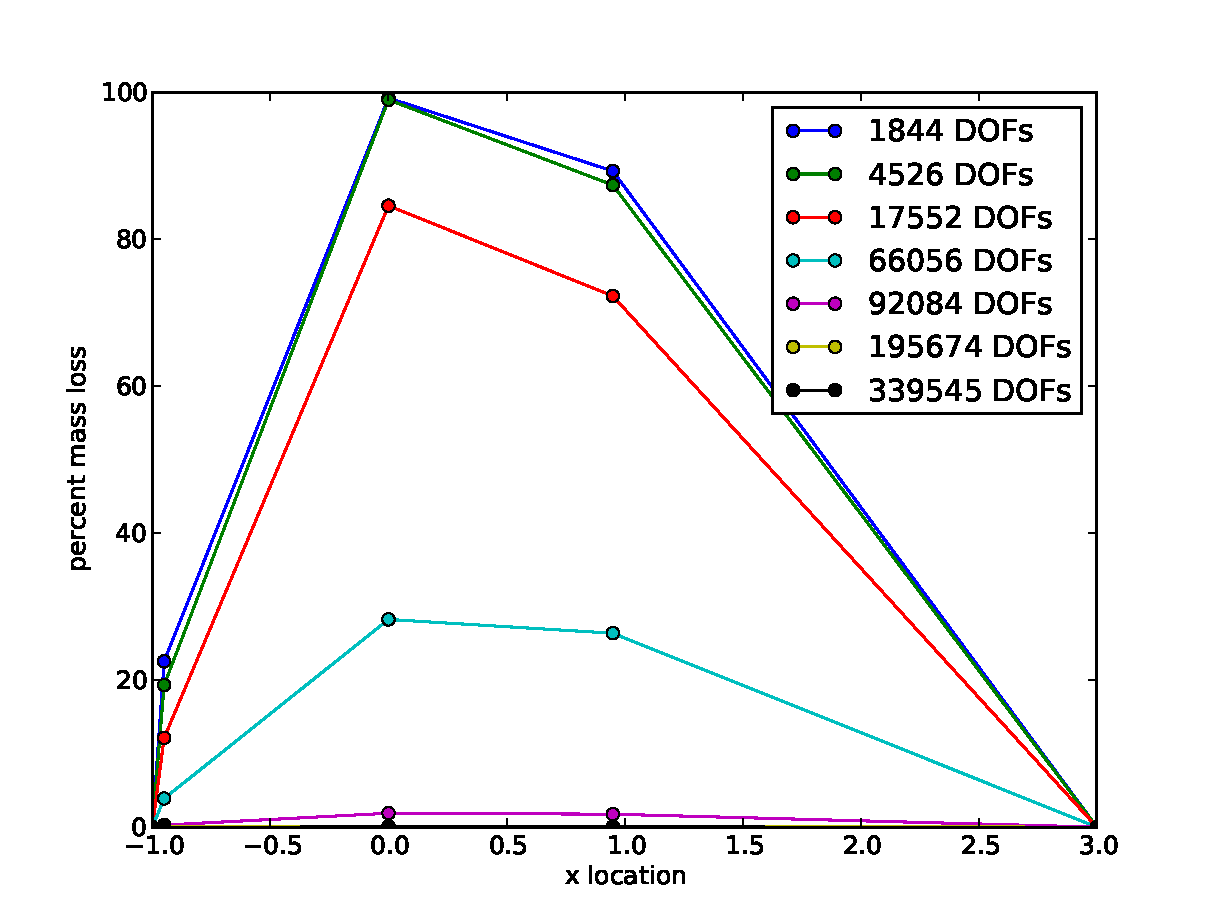
\includegraphics[width=1.1\textwidth]{StokesCylinder/MassLoss9_NC.pdf}

Nonconservative
\end{figure}
\end{column}
\begin{column}{0.49\textwidth}
\begin{figure}[t]
\centering
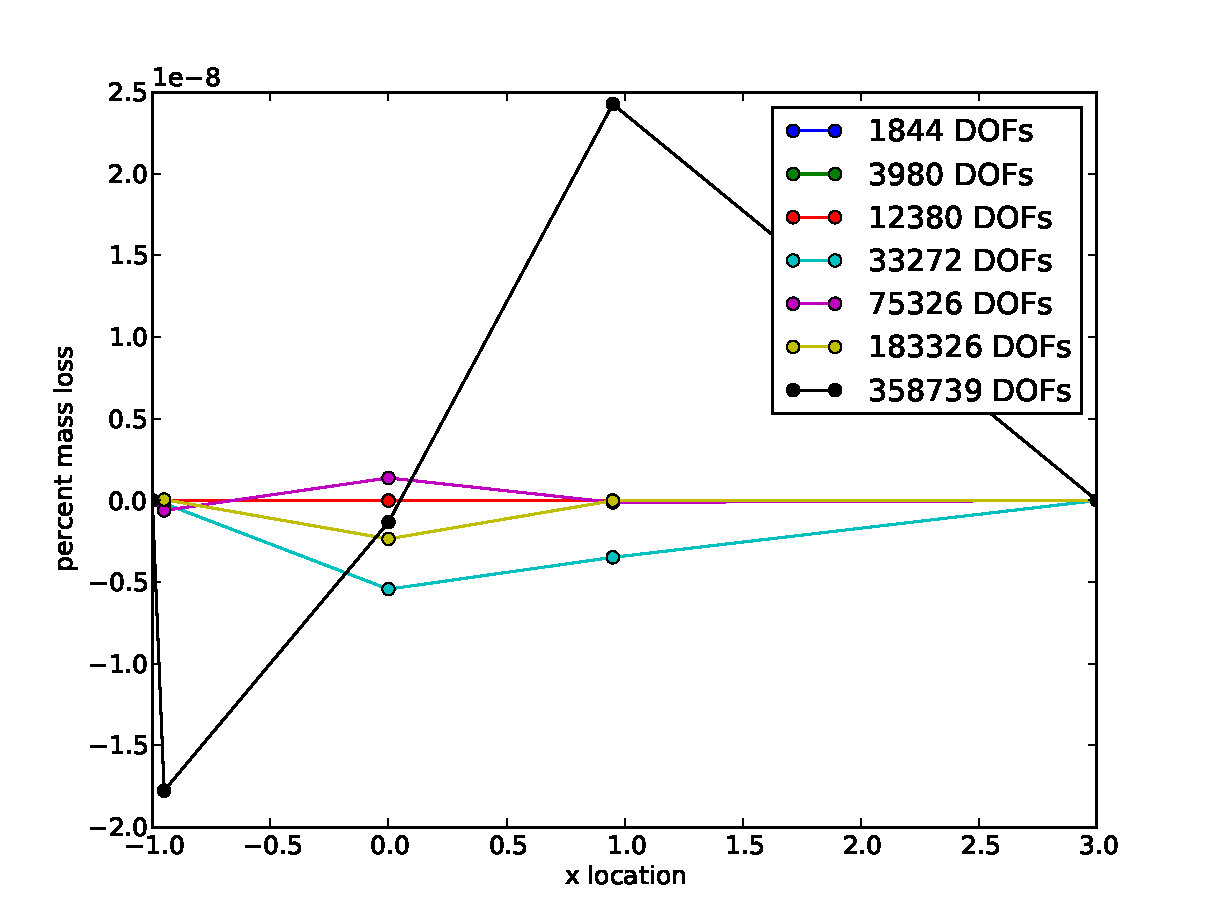
\includegraphics[width=1.1\textwidth]{StokesCylinder/MassLoss9_C.pdf}

Conservative
\end{figure}
}
\end{column}
\end{columns}
\end{frame}


%===============================================================================
% NEW SLIDE
%===============================================================================
\begin{frame}
\frametitle{Numerical Experiments}
\framesubtitle{Stokes Flow Over a Backward Facing Step}
\only<1>{
\centering
Horizontal Velocity
}
\only<2>{
\centering
Percent Mass Loss at $x=[0,0.5,\cdots,9.5,10]$
\vspace{-5ex}
}
\begin{columns}
\begin{column}{0.49\textwidth}
\only<1>{
\begin{figure}
\centering
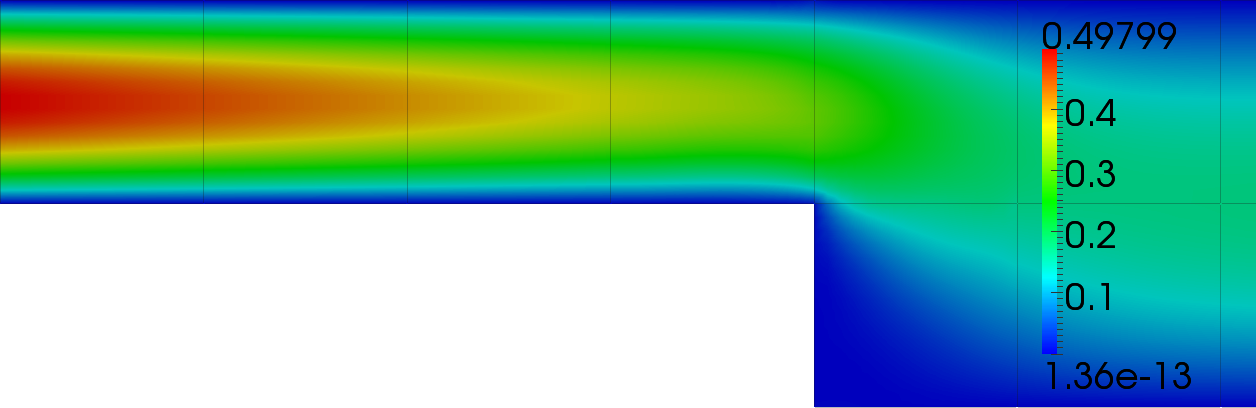
\includegraphics[width=1.0\textwidth]{StokesStep/Quartic_NC0.png}\\
\vspace{-1ex}
{\scriptsize Initial Mesh}\\
\vspace{1ex}
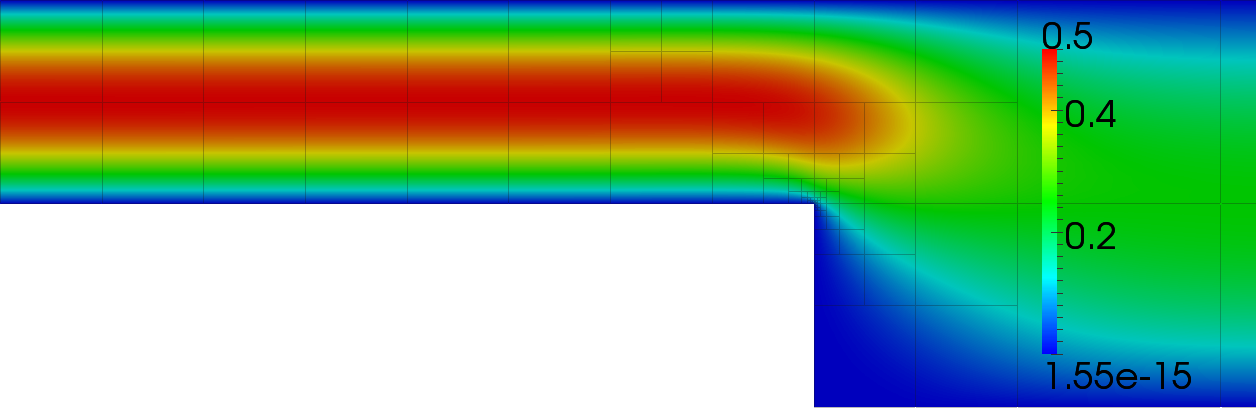
\includegraphics[width=1.0\textwidth]{StokesStep/Quartic_NC8.png}
\vspace{-1ex}
{\scriptsize 8 Refinements}
\vspace{1ex}

Nonconservative
\end{figure}
\end{column}
\begin{column}{0.49\textwidth}
\begin{figure}
\centering
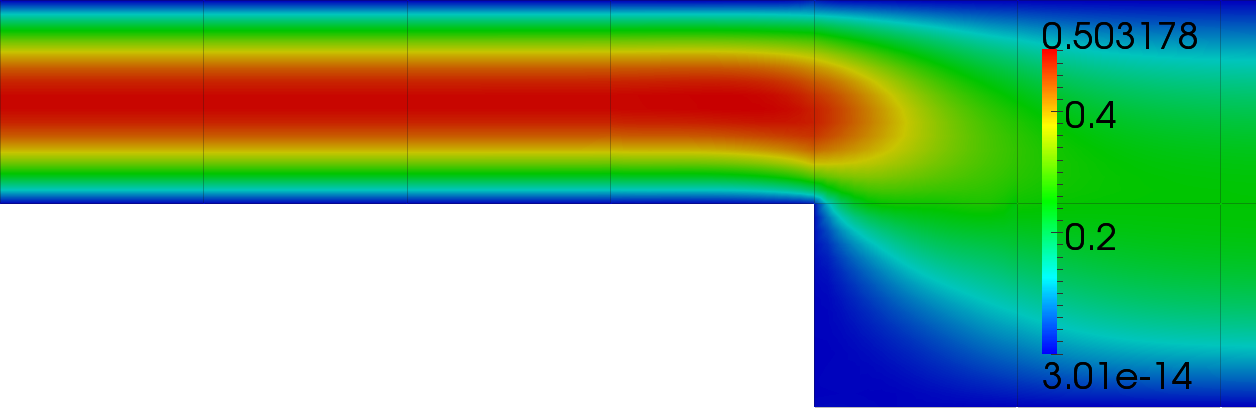
\includegraphics[width=1.0\textwidth]{StokesStep/Quartic_C0.png}\\
\vspace{-1ex}
{\scriptsize Initial Mesh}\\
\vspace{1ex}
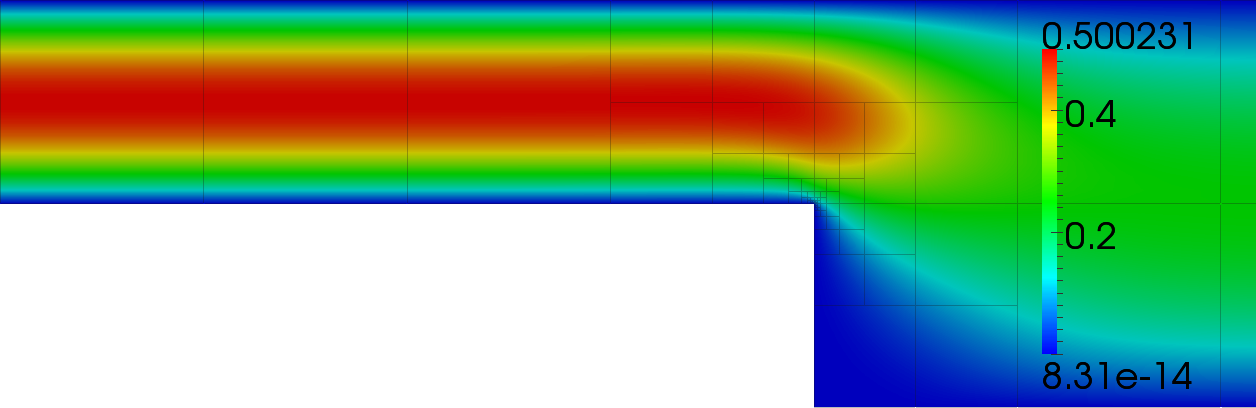
\includegraphics[width=1.0\textwidth]{StokesStep/Quartic_C8.png}
\vspace{-1ex}
{\scriptsize 8 Refinements}
\vspace{1ex}

Conservative
\end{figure}
}
\only<2>{
\begin{figure}[t]
\centering
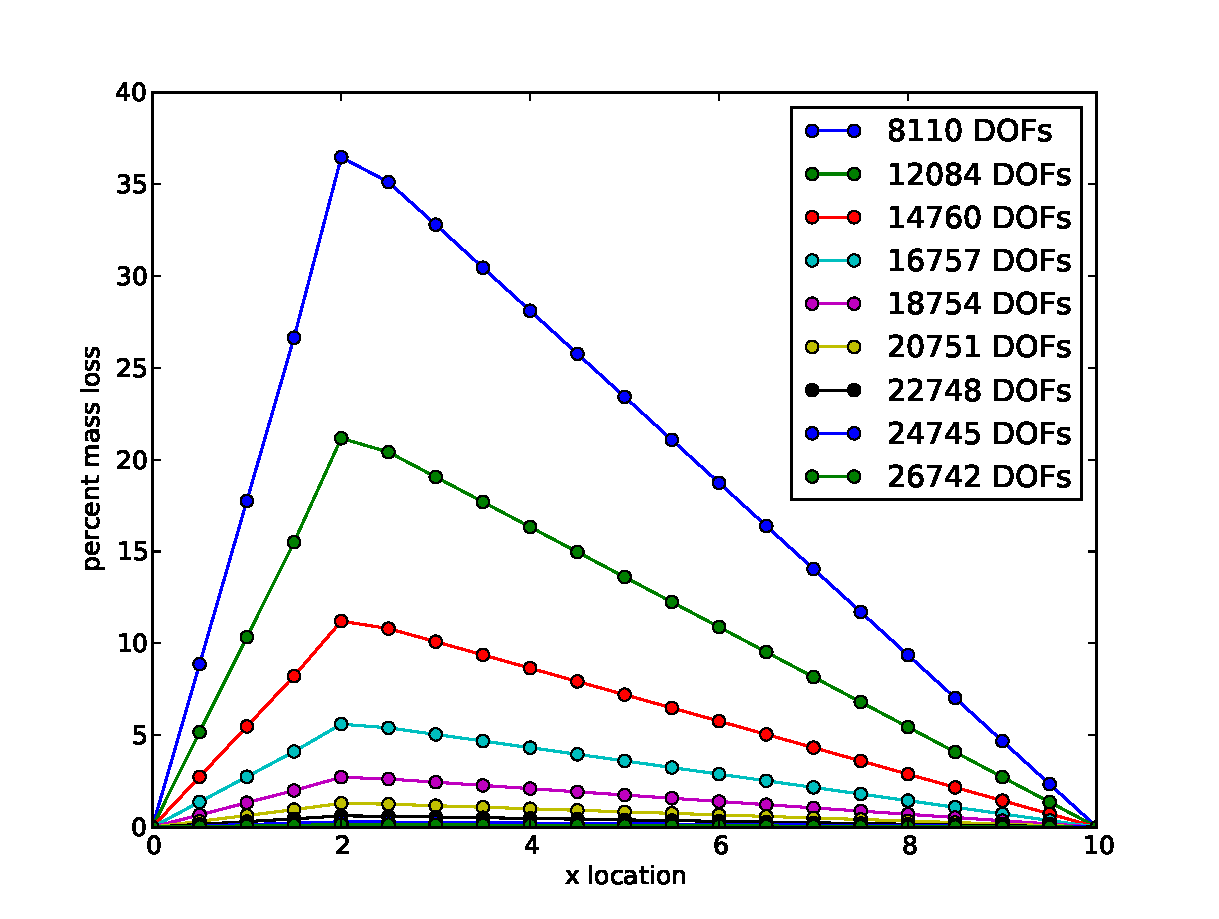
\includegraphics[width=1.1\textwidth]{StokesStep/MassLoss_NC.pdf}

Nonconservative
\end{figure}
\end{column}
\begin{column}{0.49\textwidth}
\begin{figure}[t]
\centering
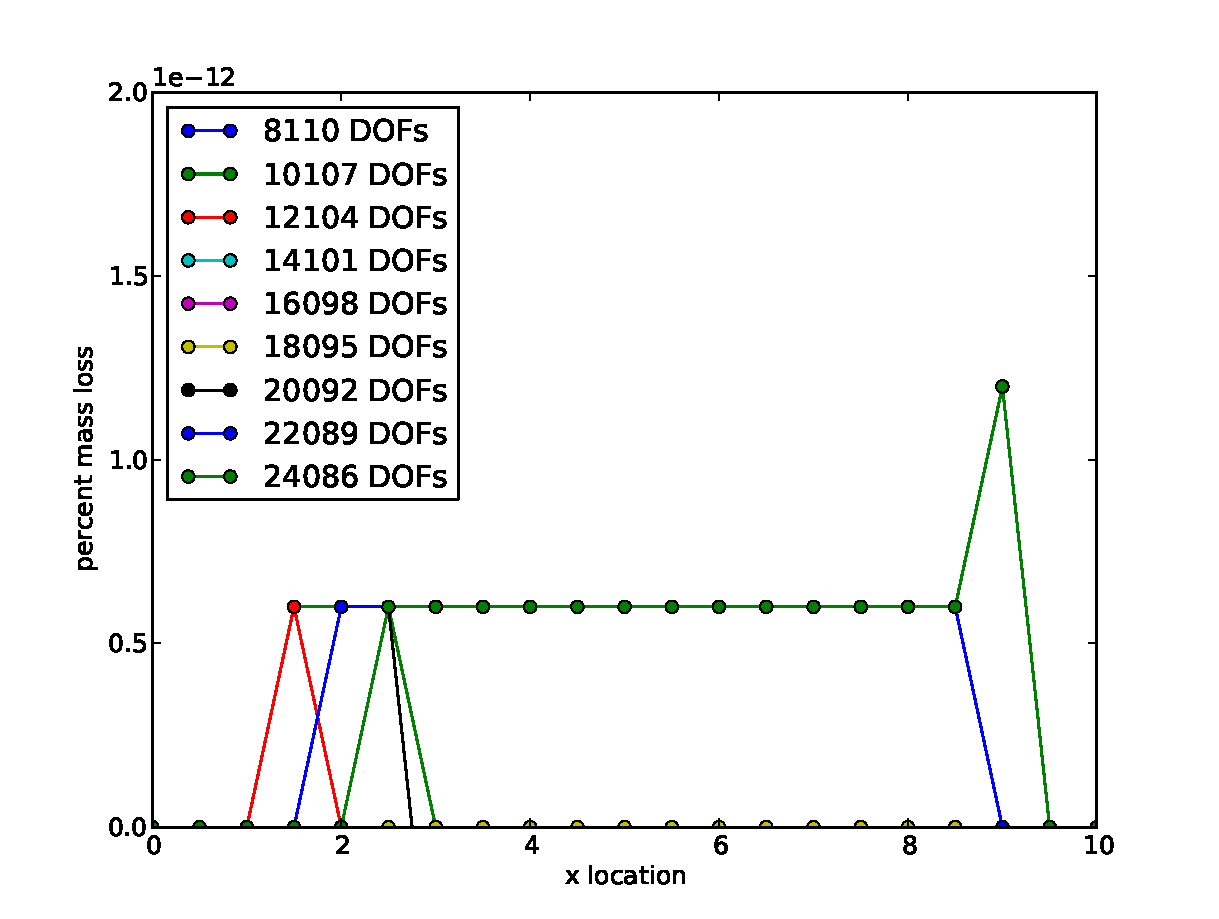
\includegraphics[width=1.1\textwidth]{StokesStep/MassLoss_C.pdf}

Conservative
\end{figure}
}
\end{column}
\end{columns}
\end{frame}


%    /$$$$$$                                                  /$$$$$$$$ /$$                        
%   /$$__  $$                                                |__  $$__/|__/                        
%  | $$  \__/  /$$$$$$   /$$$$$$   /$$$$$$$  /$$$$$$            | $$    /$$ /$$$$$$/$$$$   /$$$$$$ 
%  |  $$$$$$  /$$__  $$ |____  $$ /$$_____/ /$$__  $$ /$$$$$$   | $$   | $$| $$_  $$_  $$ /$$__  $$
%   \____  $$| $$  \ $$  /$$$$$$$| $$      | $$$$$$$$|______/   | $$   | $$| $$ \ $$ \ $$| $$$$$$$$
%   /$$  \ $$| $$  | $$ /$$__  $$| $$      | $$_____/           | $$   | $$| $$ | $$ | $$| $$_____/
%  |  $$$$$$/| $$$$$$$/|  $$$$$$$|  $$$$$$$|  $$$$$$$           | $$   | $$| $$ | $$ | $$|  $$$$$$$
%   \______/ | $$____/  \_______/ \_______/ \_______/           |__/   |__/|__/ |__/ |__/ \_______/
%            | $$                                                                                  
%            | $$                                                                                  
%            |__/  


\section{Space-Time Convection-Diffusion}
% ------------------------------------------------------------
\begin{frame}[t]
\frametitle{Space-Time DPG}
\framesubtitle{Extending DPG to Transient Problems}
\begin{itemize}
  \item Time stepping techniques are not ideally suited to highly adaptive grids
  \item Space-time FEM proposed as a solution
  \begin{itemize}
    \item[\textcolor{green}{\Checkmark}] Unified treatment of space and time
    \item[\textcolor{green}{\Checkmark}] Local space-time adaptivity (local time stepping)
    \item[\textcolor{green}{\Checkmark}] Parallel-in-time integration (space-time multigrid)
    \item[\XSolidBrush] Spatially stable FEM methods may not be stable in space-time
    \item[\XSolidBrush] Need to support higher dimensional problems
  \end{itemize}
  \item DPG provides necessary stability and adaptivity
\end{itemize}
\begin{figure}[b]
\centering
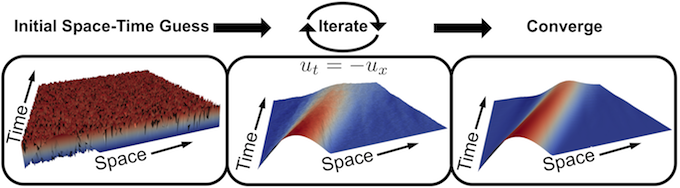
\includegraphics[width=0.8\textwidth]{Schematics/XBraid}
\\
Courtesy of XBraid by LLNL
\end{figure}
\end{frame}


% ------------------------------------------------------------
\begin{frame}[t]
\frametitle{Space-Time DPG for Convection-Diffusion}
\framesubtitle{Space-Time Divergence Form}
Equation is parabolic in space-time.
\[
\pd{u}{t}+\bfbeta\cdot\Grad u-\epsilon\Delta u=f
\]
This is just a composition of a constitutive law and conservation of mass.
\begin{align*}
\bfsigma-\epsilon\Grad u&=0\\
\pd{u}{t}+\Div\LRp{\bfbeta u-\bfsigma}&=f
\end{align*}

We can rewrite this in terms of a space-time divergence.
\begin{align*}
\frac{1}{\epsilon}\bfsigma-\Grad u &=0\\
\Gradxt\cdot\vecttwo{\bfbeta u-\bfsigma}{u}&=f
\end{align*}
\end{frame}


% ------------------------------------------------------------
\begin{frame}[t]
\frametitle{Space-Time DPG for Convection-Diffusion}
\framesubtitle{Ultra-Weak Formulation with Discontinuous Test Functions}  %% needed for proper positioning of the logo ...
% \vspace{-2ex}
Multiply by test function and integrate by parts over space-time element K.
\begin{equation*}
\begin{aligned}
\LRp{\frac{1}{\epsilon}\bfsigma,\bftau}_K+\LRp{u,\Div\bftau}_K-\LRa{\hat u,\bftau\cdot\bfn_x}_{\partial K}&=0\\
-\LRp{\vecttwo{\bfbeta u-\bfsigma}{u},\Gradxt v}_K+\LRa{\hat t,v}_{\partial K}&=f
\end{aligned}
\end{equation*}
\begin{columns}[t] % contents are top vertically aligned
\begin{column}[T]{0.4\textwidth} % each column can also be its own environment
\vspace{-3ex}
where
\vspace{-1ex}
\begin{align*}
\hat u&:=\trace(u)\\
\hat t&:=\trace(\bfbeta u-\bfsigma)\cdot\bfn_x\\
&+\trace(u)\cdot n_t
\end{align*}
\vspace{-4ex}
\begin{itemize}
  \item Trace $\hat u$ defined on spatial boundaries
  \item Flux $\hat t$ defined on all boundaries
\end{itemize}
\end{column}
\begin{column}[T]{0.6\textwidth} % alternative top-align that's better for graphics
\vspace{-2ex}
\begin{block}{Support of Trace Variables}
\begin{tikzpicture}[line cap=round,line join=round,>=triangle 45,x=2.0cm,y=2.0cm, scale=0.6, every node/.style={scale=0.6}]
\clip(-0.7,-0.6) rectangle (5.27,2.09);
\draw (0,2)-- (0,0);
\draw (0,0)-- (1,0);
\draw (1,0)-- (4,0);
\draw (4,0)-- (5,0);
\draw (5,0)-- (5,2);
\draw (5,2)-- (3,2);
\draw (3,2)-- (2,2);
\draw (2,2)-- (0,2);
\draw (1,0)-- (1.5,1);
\draw (1.5,1)-- (2,2);
\draw (1.5,1)-- (3.5,1);
\draw (3,2)-- (3.5,1);
\draw (3.5,1)-- (4,0);
\draw (-0.21,0.9) node[anchor=south west] {$\hat u$};
\draw (4.82,0.9) node[anchor=south west] {$\hat u$};
\draw (3.5,0.45) node[anchor=south west] {$\hat u$};
\draw (1.0,0.45) node[anchor=south west] {$\hat u$};
\draw (1.5,1.4) node[anchor=south west] {$\hat u$};
\draw (3.0,1.4) node[anchor=south west] {$\hat u$};
\draw (0.05,0.9) node[anchor=south west] {$\hat t$};
\draw (1.40,0.45) node[anchor=south west] {$\hat t$};
\draw (3.79,0.45) node[anchor=south west] {$\hat t$};
\draw (2.47,1.0) node[anchor=south west] {$\hat t$};
\draw (3.33,1.4) node[anchor=south west] {$\hat t$};
\draw (1.89,1.4) node[anchor=south west] {$\hat t$};
\draw (5.07,0.9) node[anchor=south west] {$\hat t$};
\draw (4.44,0.0) node[anchor=south west] {$\hat t$};
\draw (2.46,0.0) node[anchor=south west] {$\hat t$};
\draw (0.45,0.0) node[anchor=south west] {$\hat t$};
\draw (2.44,1.7) node[anchor=south west] {$\hat t$};
\draw (0.76,1.7) node[anchor=south west] {$\hat t$};
\draw (4.21,1.7) node[anchor=south west] {$\hat t$};
\draw [->] (-0.5,-0.5) -- (-0.5,0);
\draw [->] (-0.5,-0.5) -- (0,-0.5);
\draw (-0.54,0.29) node[anchor=north west] {$t$};
\draw (0.07,-0.35) node[anchor=north west] {$x$};
\end{tikzpicture}
\end{block}
\end{column}
\end{columns}
\end{frame}



% ------------------------------------------------------------
\begin{frame}[t]
\frametitle{Space-Time Convection-Diffusion}
\framesubtitle{$L^2$ Equivalent Norms}
% \vspace{-5ex}
\begin{columns}[t]
\begin{column}{0.5\textwidth}
\vspace{-3ex}

Bilinear form with group variables:
\[
b\LRp{\LRp{u,\hat u},v} = \LRp{u,A^*_h v}_{\LOmega} + \LRa{\uh, \jump{v}}_{\Gh}
\]
For conforming $v^*$ satisfying $A^* v^* = u$
\begin{align*}
&\norm{u}_{\LOmega}^2= b(u,v^*)
=\frac{b(u,v^*)}{\norm{v^*}_V} \norm{v^*}_V\\
&\quad\leq\sup_{v^*\neq0}\frac{|b(u,v^*)|}{\norm{v^*}}\norm{v^*}
=\norm{u}_E \norm{v^*}_V
\end{align*}
% If our test norm is bounded by $\norm{u}_{\LOmega}$,
% we can quarantee that 
% If $\norm{v^*}_V\lesssim\norm{u}_{L^2(\Omega_h)}$
% then $\Rightarrow\norm{u}_{L^2(\Omega_h)}\lesssim\norm{u}_E$.
Necessary robustness condition:
\begin{align*}
&\norm{v^*}_V\lesssim\norm{u}_{L^2(\Omega_h)}\\
&\quad\Rightarrow\norm{u}_{L^2(\Omega_h)}\lesssim\norm{u}_E
\end{align*}
\end{column}
\begin{column}{0.5\textwidth}
\vspace{-3ex}
\centering

Analytical Solution
\small{
\begin{align*}
e^{-lt}(e^{\lambda_1(x-1)}-e^{\lambda_2(x-1)})\\
+\LRp{1-e^{\frac{1}{\epsilon}x}}
\end{align*}
}
% where $l=3, \quad\epsilon = 10^{-2}$
\vspace{-2ex}
\begin{figure}[t]
\centering
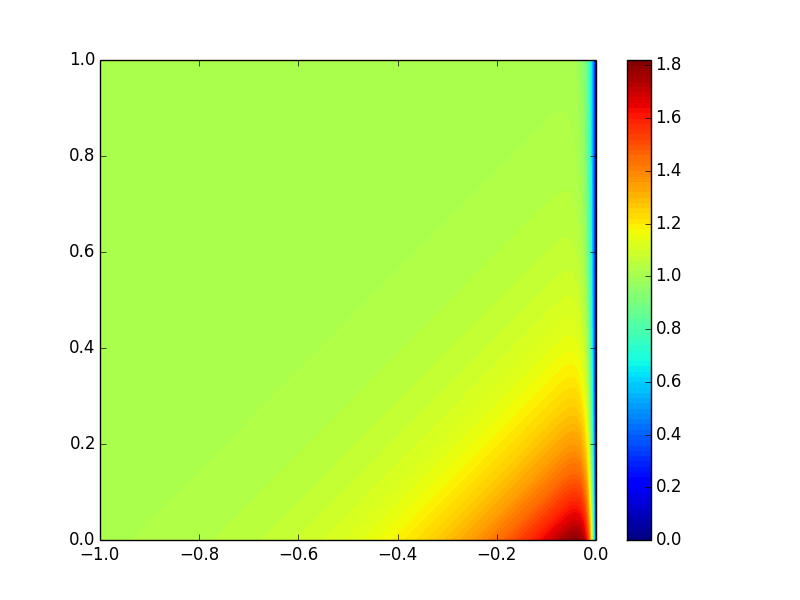
\includegraphics[width=0.8\textwidth]{Confusion/Robustness/1d_problem.png}
\end{figure}
\end{column}
\end{columns}
\end{frame}

% ------------------------------------------------------------
\begin{frame}[t]
\frametitle{Space-Time Convection-Diffusion}
\framesubtitle{$L^2$ Equivalent Norms}
A norm should be: bounded by $\norm{u}_{\LOmega}$, have good conditioning, not produce boundary layers in the optimal test function.
\vspace{-5ex}
\begin{columns}[t]
\begin{column}{0.5\textwidth}
\begin{figure}[t]
\centering
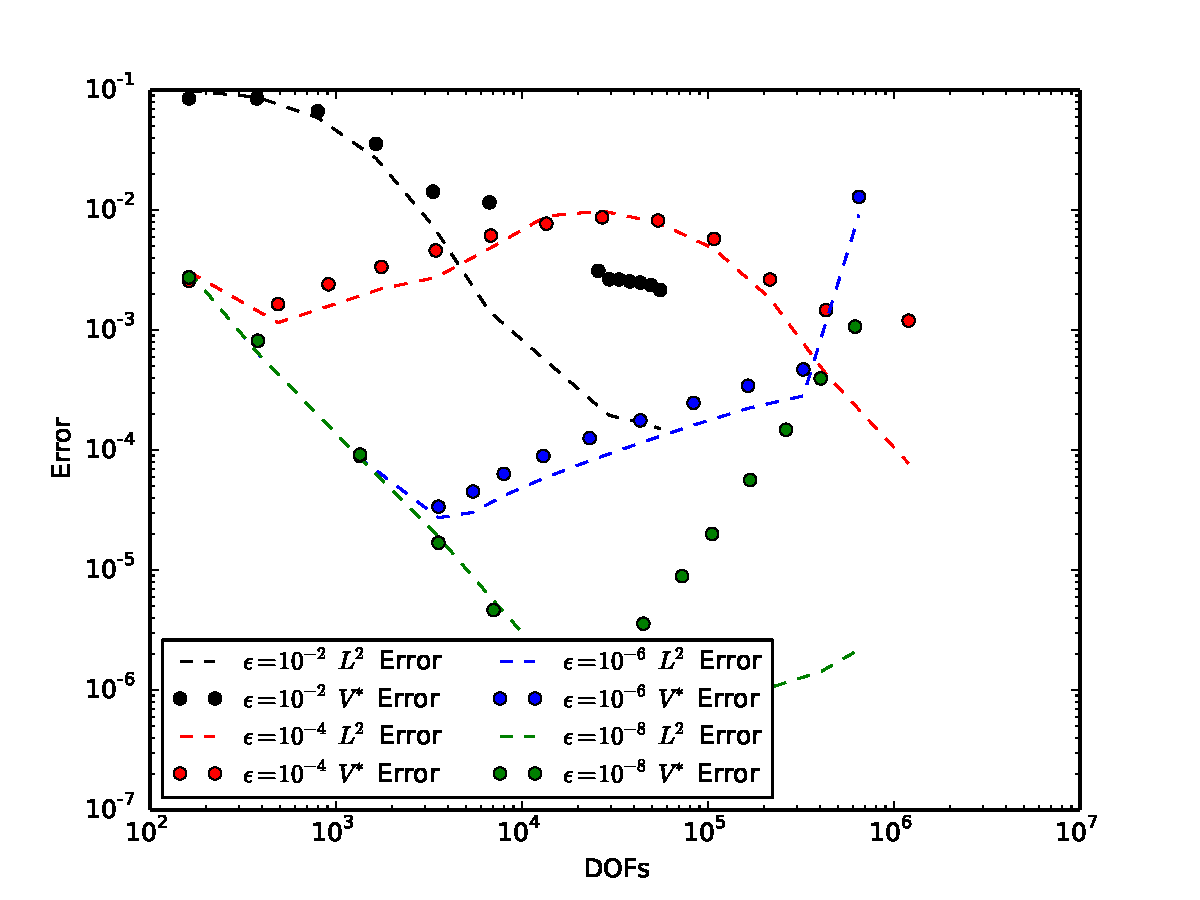
\includegraphics[width=\textwidth]{Confusion/Robustness/convergence1D_p2_graph.pdf}
\end{figure}
\vspace{-5ex}
\small{
\begin{align*}
\norm{(v,\bftau)}^2&=
\norm{\Div\bftau-\tilde\bfbeta\cdot\Gradxt v}^2\\
&+\norm{\frac{1}{\epsilon}\bftau+\Grad v}^2
+\norm{v}^2
+\norm{\bftau}^2
\end{align*}
}
\end{column}
\begin{column}{0.5\textwidth}
\begin{figure}[t]
\centering
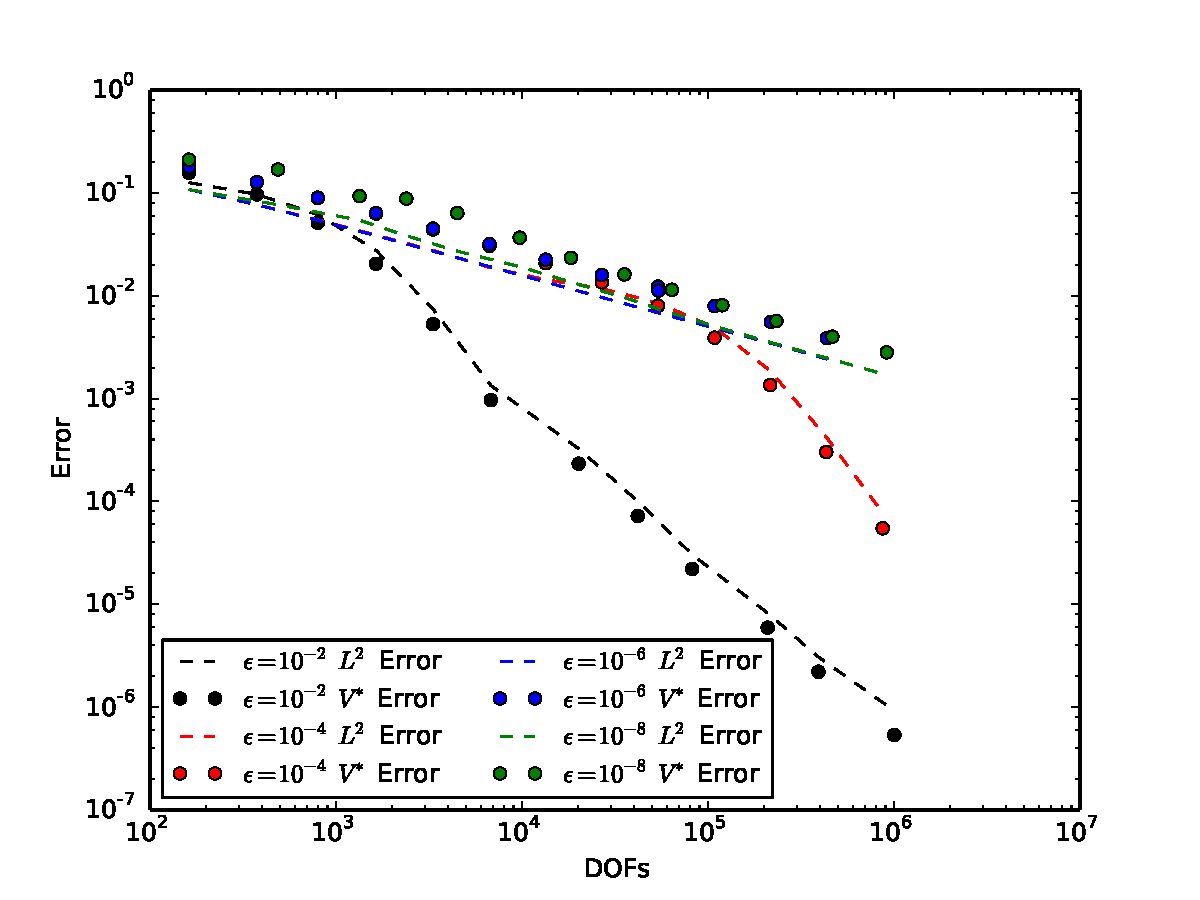
\includegraphics[width=\textwidth]{Confusion/Robustness/convergence1D_p2_robust.pdf}
\end{figure}
\vspace{-5ex}
\small{
\begin{align*}
\norm{(v,\bftau)}^2&=
\norm{\Div\bftau-\tilde\bfbeta\cdot\Gradxt v}^2\\
&+\min\LRp{\frac{1}{h^2},\frac{1}{\epsilon}}\norm{\bftau}^2\\
&+\epsilon\norm{\Grad v}^2
+\norm{\bfbeta\cdot\Grad v}^2
+\norm{v}^2
\end{align*}
}
\end{column}
\end{columns}
\end{frame}

% ------------------------------------------------------------
\begin{frame}[t]
\frametitle{Steady Convection-Diffusion}
\framesubtitle{Ideal Optimal Shape Functions}
\vspace{-3ex}
\begin{columns}
\begin{column}{0.5\textwidth}
\begin{figure}[t]
\centering
Graph Norm
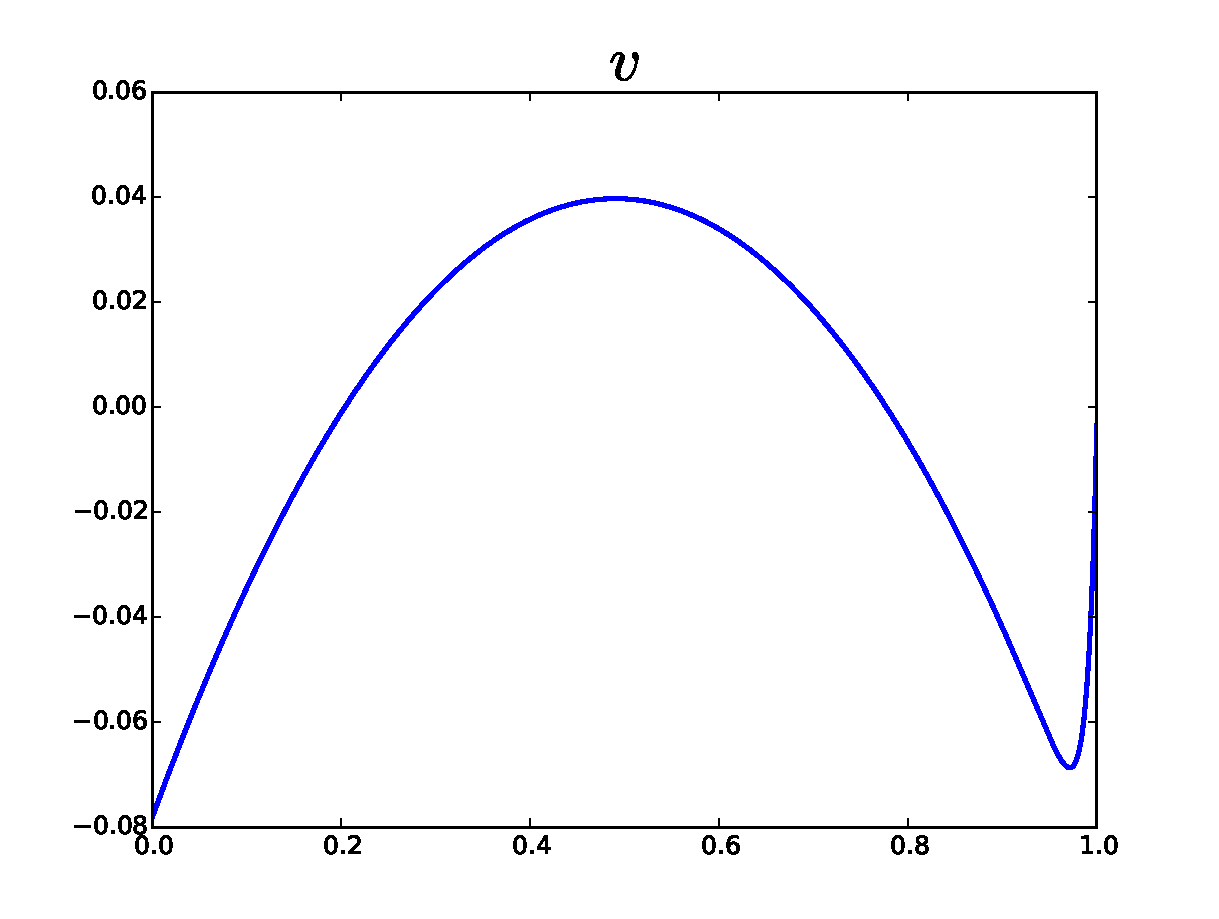
\includegraphics[width=0.8\textwidth]{OptimalTestFunctions/uLinear_1e-2/steady/graph_steady_v.pdf}\\
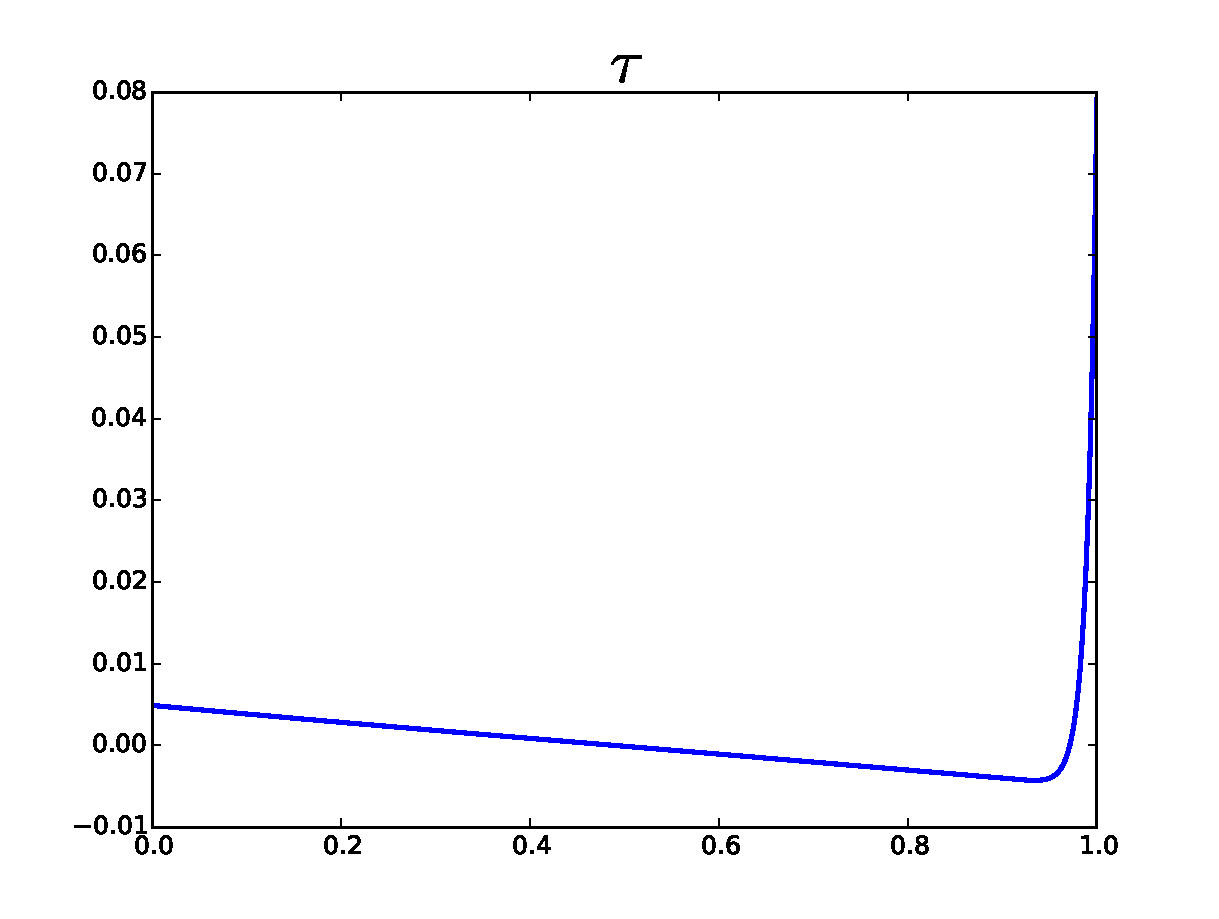
\includegraphics[width=0.8\textwidth]{OptimalTestFunctions/uLinear_1e-2/steady/graph_steady_tau.pdf}
% 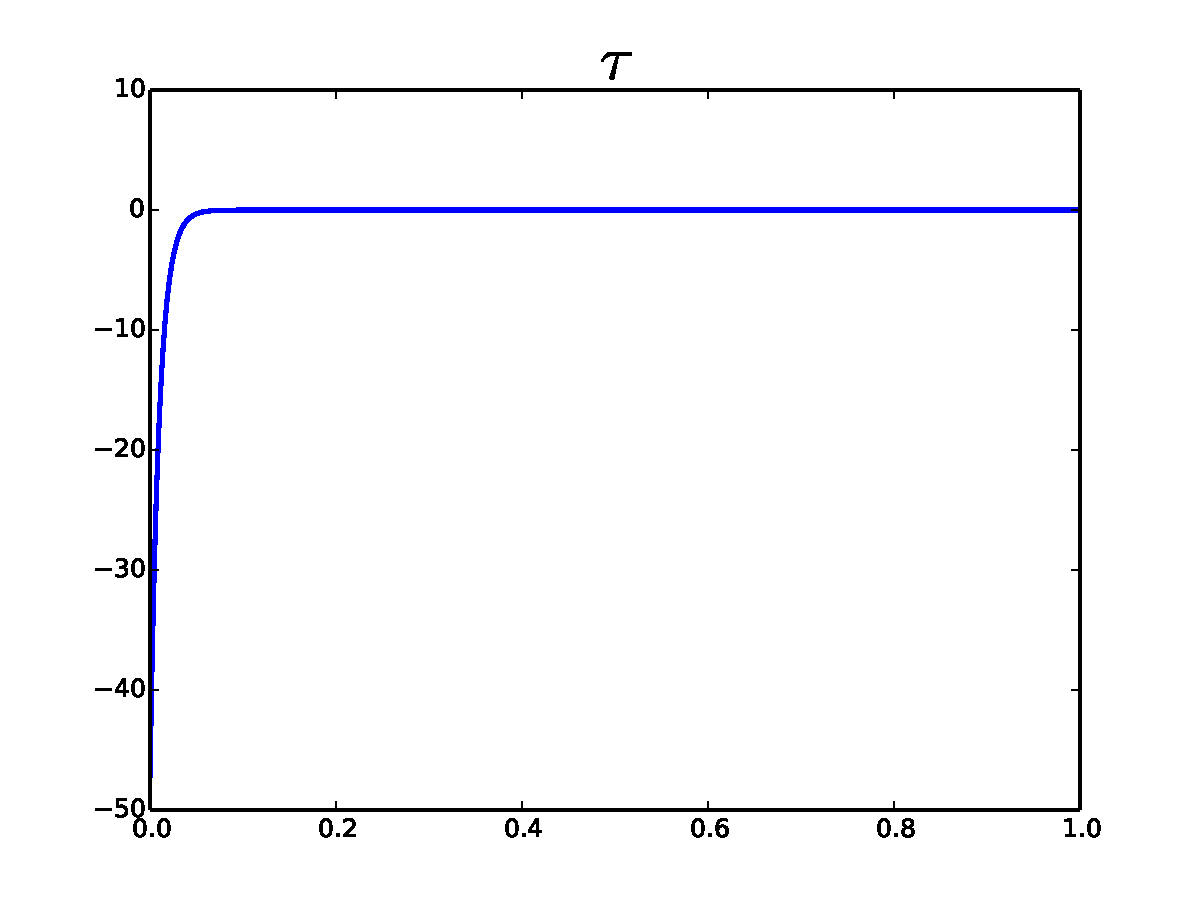
\includegraphics[width=0.8\textwidth]{OptimalTestFunctions/Graph_tau}
\end{figure}
\end{column}
\begin{column}{0.5\textwidth}
\begin{figure}[t]
\centering
Coupled Robust Norm
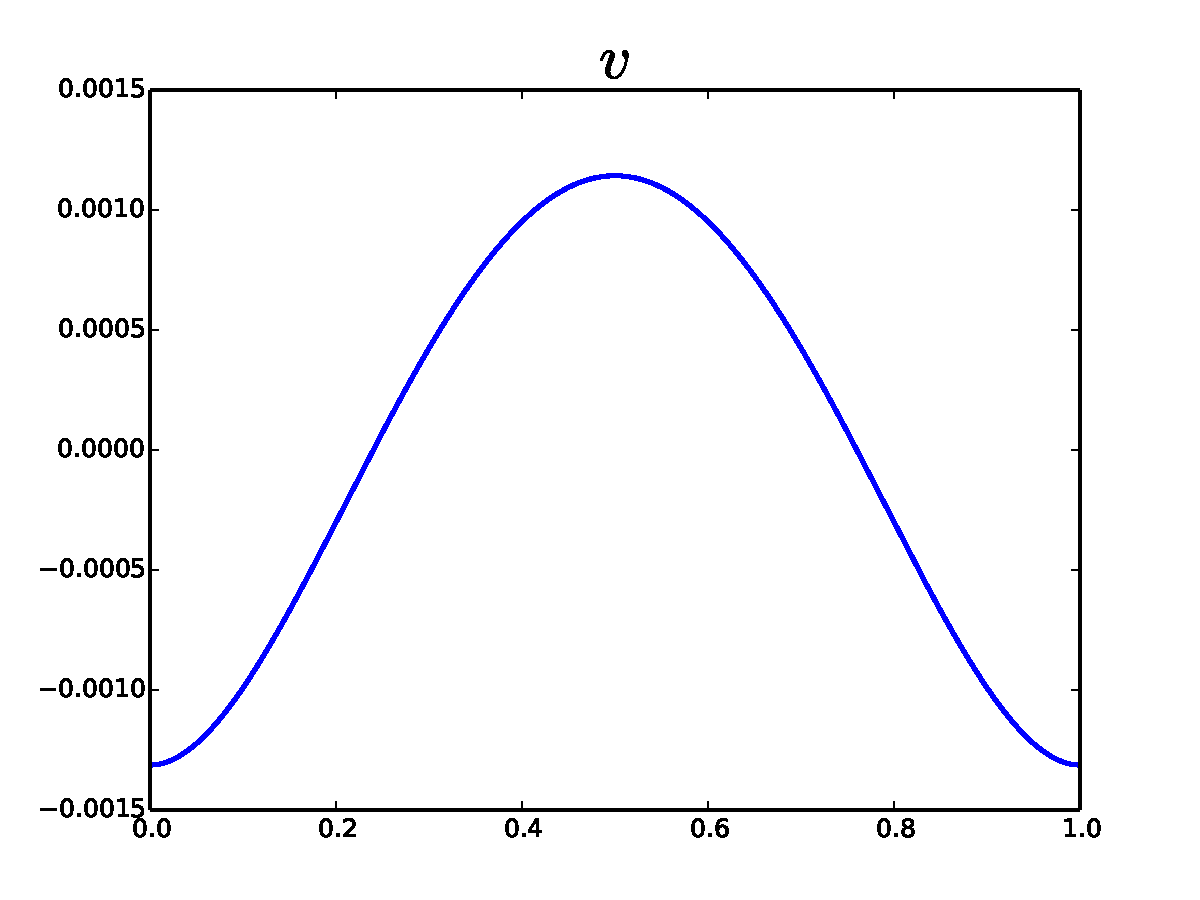
\includegraphics[width=0.8\textwidth]{OptimalTestFunctions/uLinear_1e-2/steady/coupledrobust_steady_v.pdf}\\
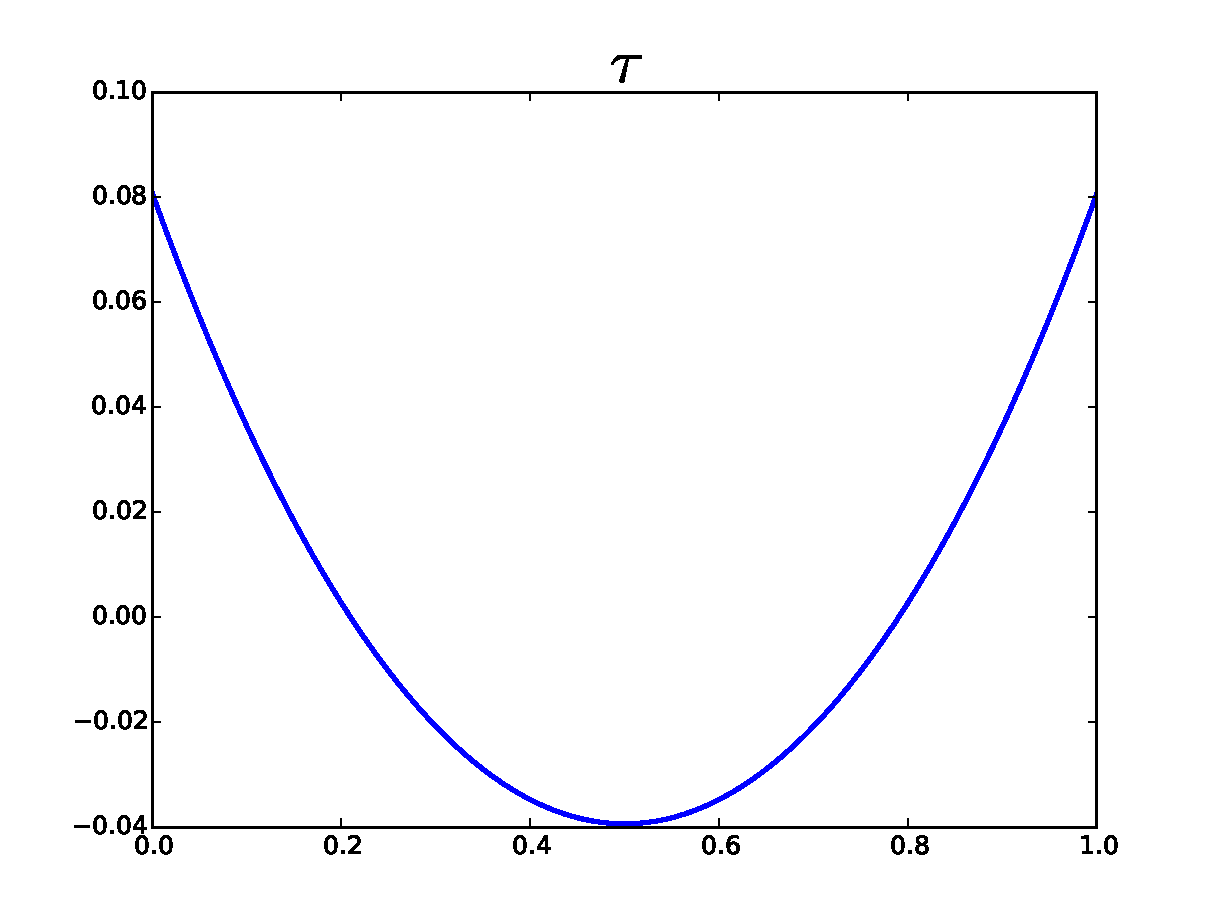
\includegraphics[width=0.8\textwidth]{OptimalTestFunctions/uLinear_1e-2/steady/coupledrobust_steady_tau.pdf}
% 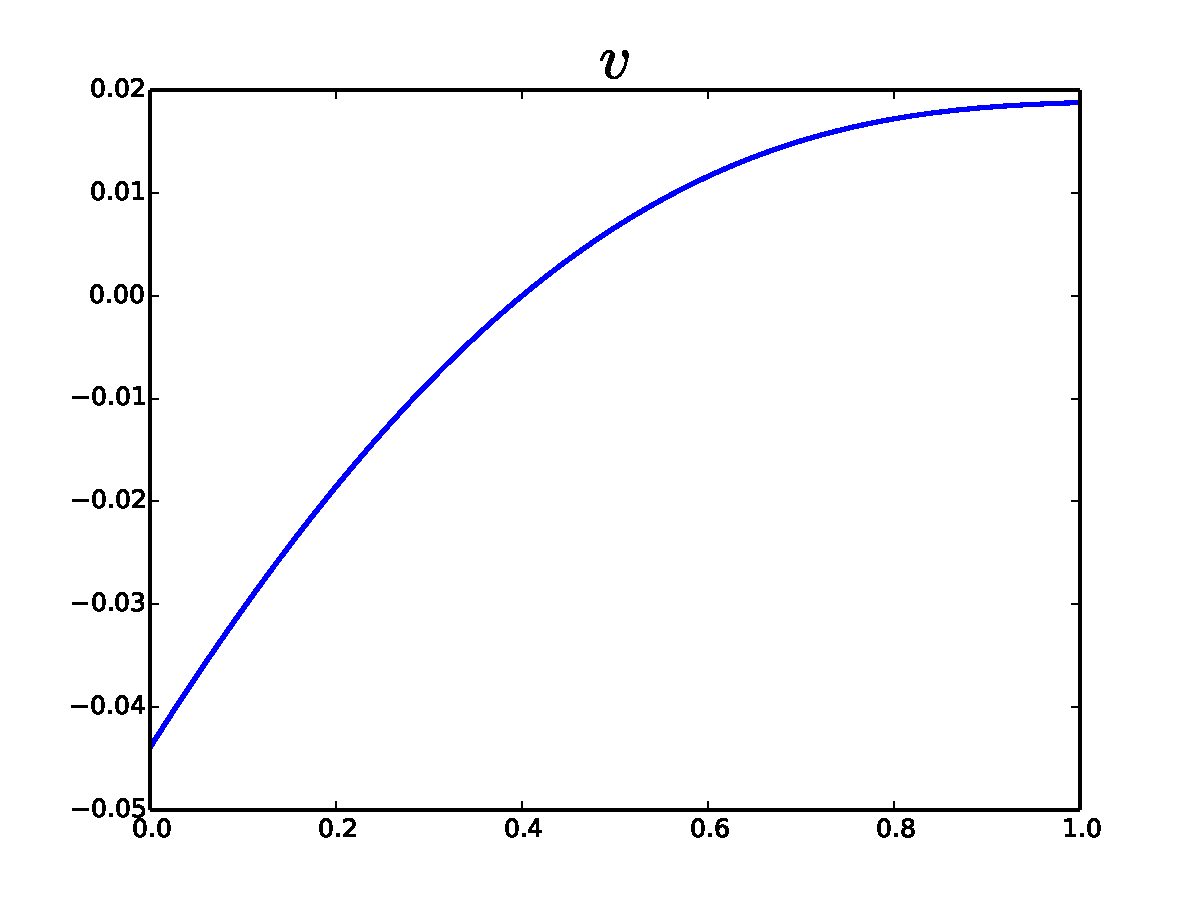
\includegraphics[width=0.8\textwidth]{OptimalTestFunctions/Robust_v}\\
% 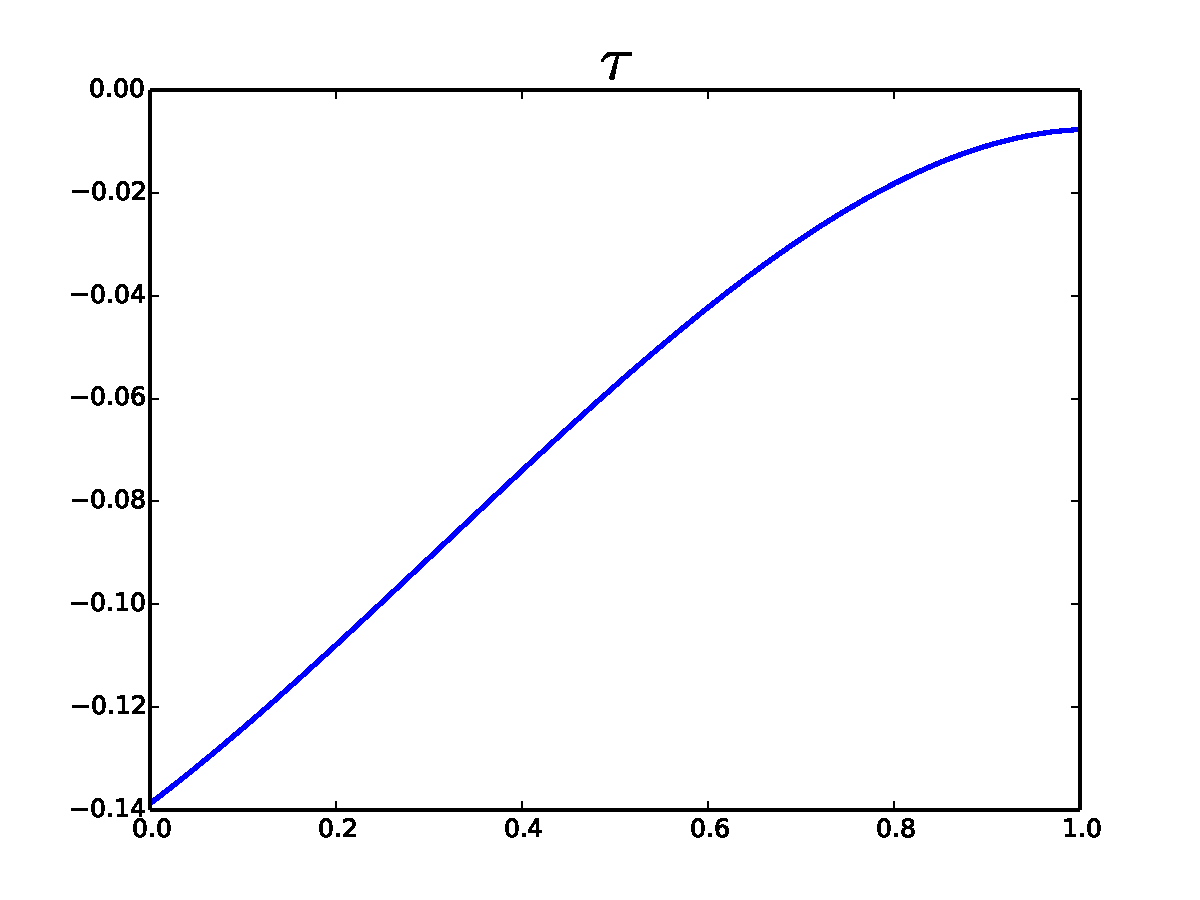
\includegraphics[width=0.8\textwidth]{OptimalTestFunctions/Robust_tau}
\end{figure}
\end{column}
\end{columns}
\end{frame}

% ------------------------------------------------------------
\begin{frame}[t]
\frametitle{Steady Convection-Diffusion}
\framesubtitle{Approximated ($p=3$) Optimal Shape Functions}
\vspace{-3ex}
\begin{columns}
\begin{column}{0.5\textwidth}
\begin{figure}[t]
\centering
Graph Norm
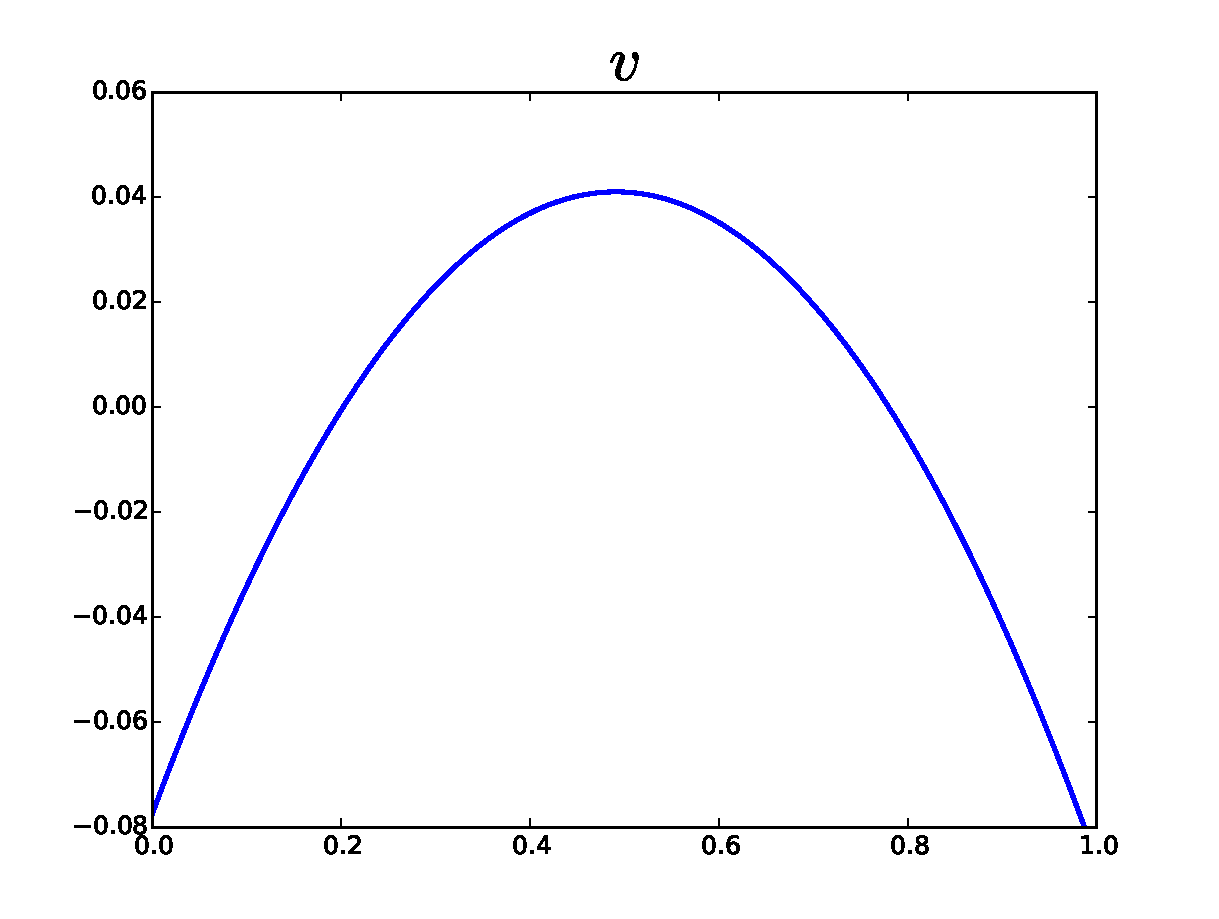
\includegraphics[width=0.8\textwidth]{OptimalTestFunctions/uLinear_1e-2/steady/graph_steady_v_approx3.pdf}\\
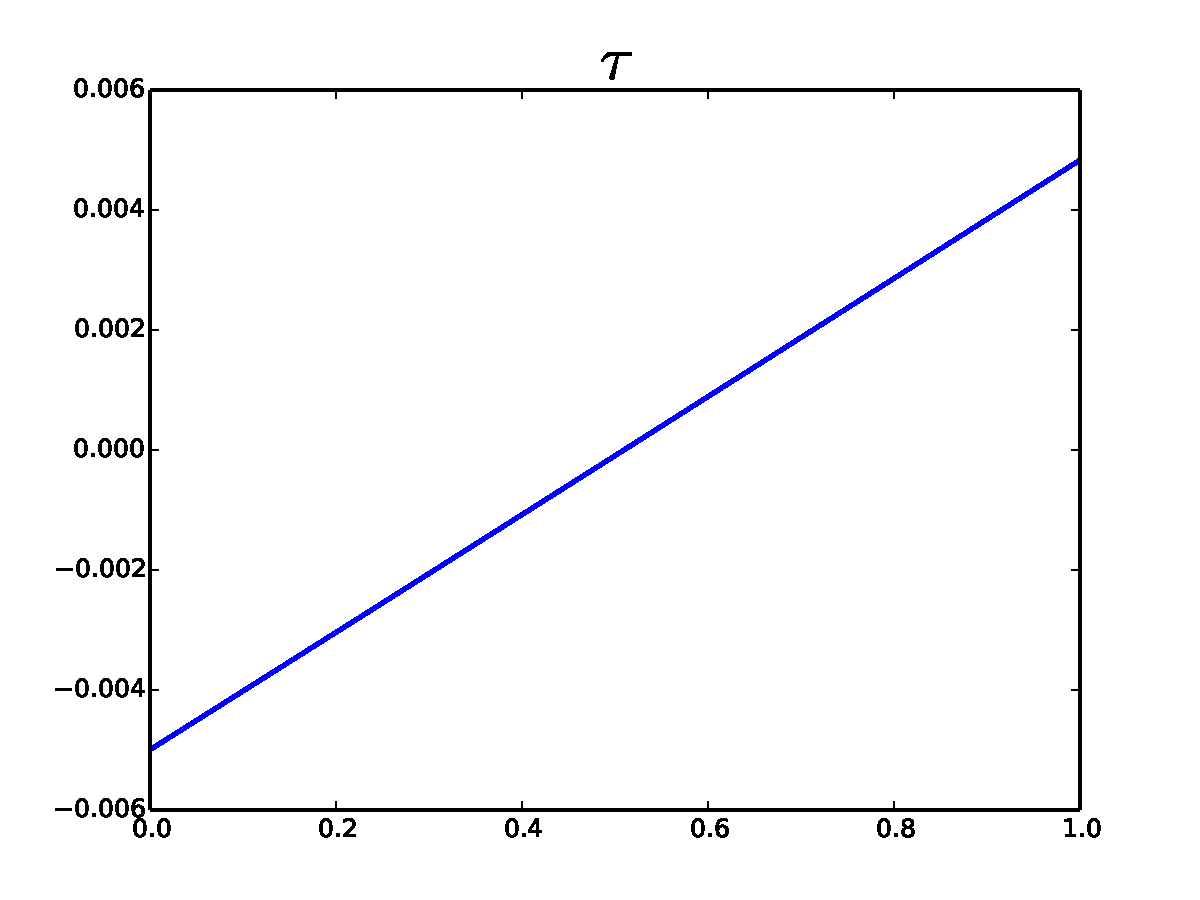
\includegraphics[width=0.8\textwidth]{OptimalTestFunctions/uLinear_1e-2/steady/graph_steady_tau_approx3.pdf}
\end{figure}
\end{column}
\begin{column}{0.5\textwidth}
\begin{figure}[t]
\centering
Coupled Robust Norm
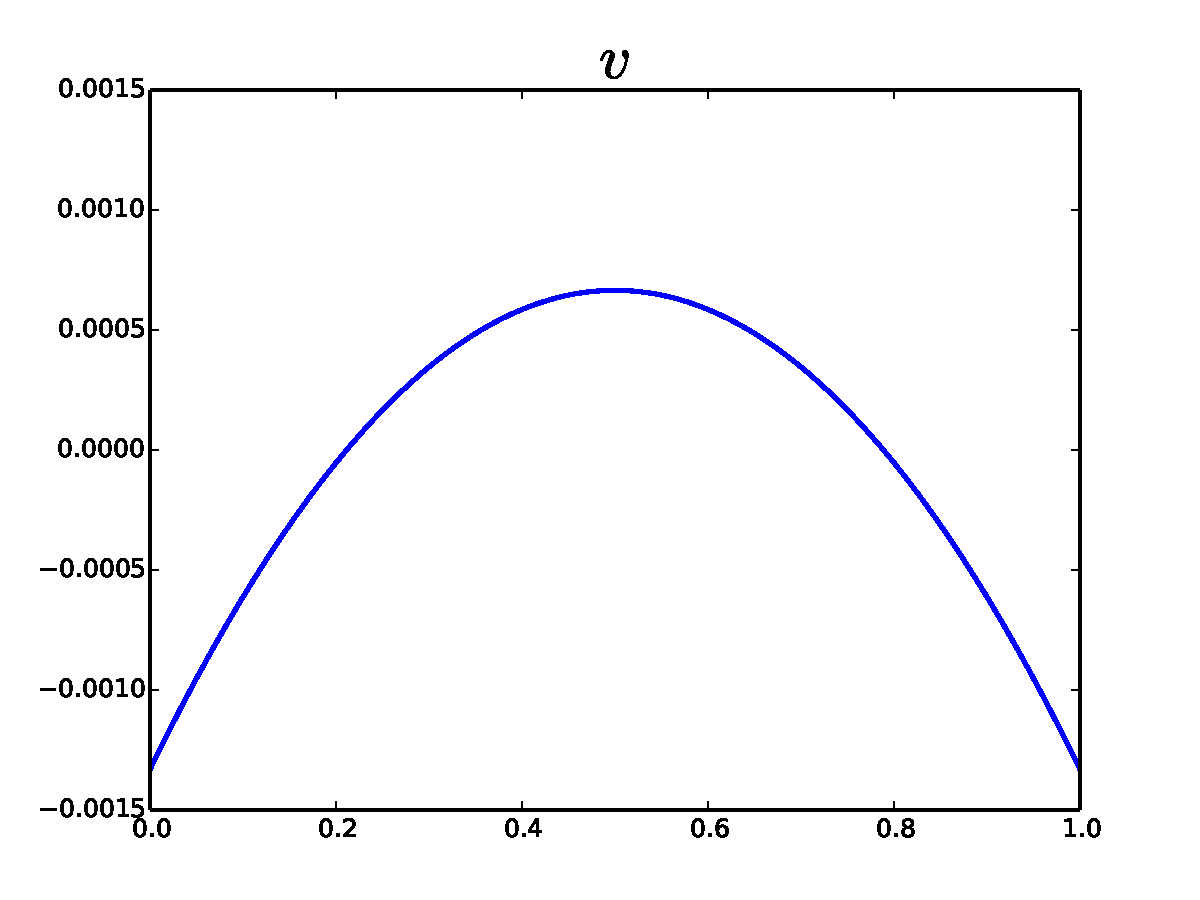
\includegraphics[width=0.8\textwidth]{OptimalTestFunctions/uLinear_1e-2/steady/coupledrobust_steady_v_approx3.pdf}\\
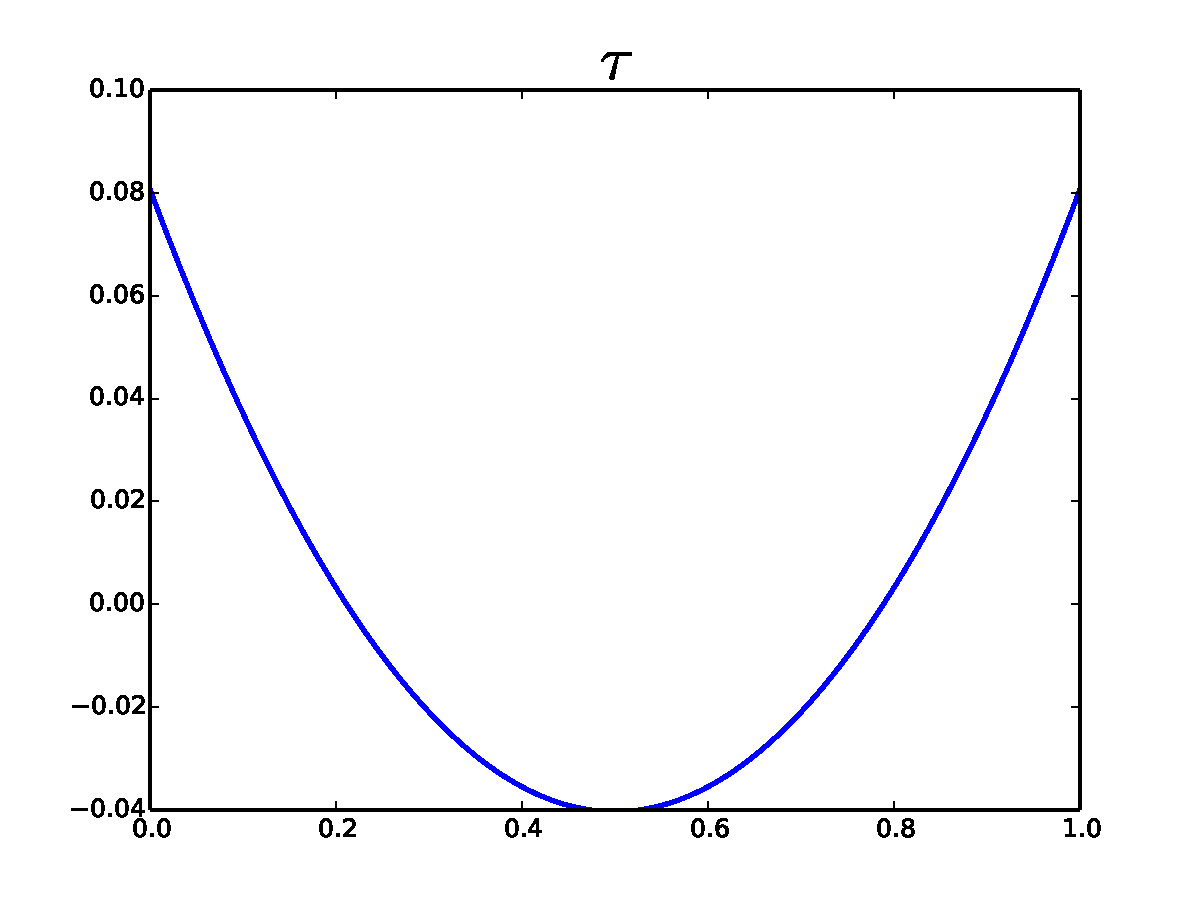
\includegraphics[width=0.8\textwidth]{OptimalTestFunctions/uLinear_1e-2/steady/coupledrobust_steady_tau_approx3.pdf}
\end{figure}
\end{column}
\end{columns}
\end{frame}

% ------------------------------------------------------------
\begin{frame}[t]
\frametitle{Steady Convection-Diffusion}
\framesubtitle{Two Robust Norms for Steady Convection-Diffusion}

The following norms are robust for steady convection-diffusion.

The robust norm was derived in \footfullcite{ChanHeuerThanhDemkowicz2012}:
\begin{align*}
\norm{(v,\bftau)}^2&=
\norm{\bfbeta\cdot\Grad v}^2
+\epsilon\norm{\Grad v}^2
+\min\LRp{\frac{\epsilon}{h^2},1}\norm{v}^2\\
&+\norm{\Div\bftau}^2
+\min\LRp{\frac{1}{h^2},\frac{1}{\epsilon}}\norm{\bftau}^2\,.
\end{align*}
The case for the coupled robust norm was made in \footfullcite{JesseDissertation}:
\begin{align*}
\norm{(v,\bftau)}^2&=
\norm{\bfbeta\cdot\Grad v}^2
+\epsilon\norm{\Grad v}^2
+\min\LRp{\frac{\epsilon}{h^2},1}\norm{v}^2\\
&+\norm{\Div\bftau-\bfbeta\cdot\Grad v}^2
+\min\LRp{\frac{1}{h^2},\frac{1}{\epsilon}}\norm{\bftau}^2\,.
\end{align*}
\end{frame}

% ------------------------------------------------------------
\begin{frame}[t]
\frametitle{Space-Time Convection-Diffusion}
\framesubtitle{Two Robust Norms for Transient Convection-Diffusion}
Let $\tilde\bfbeta:=\vecttwo{\bfbeta}{1}$ and $\Gradxt v:=\vecttwo{\Grad v}{\pd{v}{t}}$.

The following norms are robust for space-time convection-diffusion.

Robust Norm:
\begin{align*}
\norm{(v,\bftau)}^2&=
\norm{\textcolor{red}{\tilde\bfbeta\cdot\Gradxt v}}^2
+\epsilon\norm{\Grad v}^2
+\min\LRp{\frac{\epsilon}{h^2},1}\norm{v}^2\\
&+\norm{\Div\bftau}^2
+\min\LRp{\frac{1}{h^2},\frac{1}{\epsilon}}\norm{\bftau}^2\,.
\end{align*}
Coupled Robust Norm
\begin{align*}
\norm{(v,\bftau)}^2&=
\norm{\textcolor{red}{\tilde\bfbeta\cdot\Gradxt v}}^2
+\epsilon\norm{\Grad v}^2
+\min\LRp{\frac{\epsilon}{h^2},1}\norm{v}^2\\
&+\norm{\Div\bftau-\textcolor{red}{\tilde\bfbeta\cdot\Gradxt v}}^2
+\min\LRp{\frac{1}{h^2},\frac{1}{\epsilon}}\norm{\bftau}^2\,.
\end{align*}
\end{frame}

% ------------------------------------------------------------
\begin{frame}[t]
\frametitle{Robust Norms for Transient Convection-Diffusion}
\framesubtitle{Adjoint Operator}
Consider the problem with homogeneous boundary conditions
\begin{align*}
\frac{1}{\epsilon}\bfsigma-\Grad u &=0\\
\tilde\bfbeta\cdot\Gradxt u - \Div\bfsigma &= f\\
% \Divxt\vecttwo{\bfbeta u-\bfsigma}{u}&=f\\
\beta_n u-\epsilon\pd{u}{n} &= 0 \text{ on } \Gamma_-\\
u &= 0 \text{ on } \Gamma_+\\
u &= u_0 \text{ on } \Gamma_0.
\end{align*}
The adjoint operator $A^*$ is given by 
\[
A^*(v,\bftau)=\LRp{\frac{1}{\epsilon}\bftau+\Grad v,-\tilde\bfbeta\cdot\Gradxt v+\Div\bftau}\,.
\]
\end{frame}

% ------------------------------------------------------------
\begin{frame}[t]
\frametitle{Robust Norms for Transient Convection-Diffusion}
\framesubtitle{Controlling Different Field Variables}
We decompose the continuous adjoint problem
$
A^*(\bftau,v)=(\bfsigma,u)
$
into
\begin{block}{Continuous part with forcing $u$}
\begin{columns}[t]
\begin{column}{0.4\textwidth}
\begin{align*}
\frac{1}{\epsilon}\bftau_1+\Grad v_1 &=0\\
-\tilde\bfbeta\cdot\Gradxt v_1 + \Div\bftau_1 &= u\\
\end{align*}
\end{column}
\begin{column}{0.4\textwidth}
\begin{align*}
\bftau_1\cdot\bfn_x &= 0 \text{ on } \Gamma_-\\
v_1 &= 0 \text{ on } \Gamma_+\\
v_1 &= 0 \text{ on } \Gamma_T
\end{align*}
\end{column}
\end{columns}
\end{block}
\begin{block}{Continuous part with forcing $\bfsigma$}
\begin{columns}[t]
\begin{column}{0.4\textwidth}
\begin{align*}
\frac{1}{\epsilon}\bftau_2+\Grad v_2 &=\bfsigma\\
-\tilde\bfbeta\cdot\Gradxt v_2 + \Div\bftau_2 &= 0\\
\end{align*}
\end{column}
\begin{column}{0.4\textwidth}
\begin{align*}
\bftau_2\cdot\bfn_x &= 0 \text{ on } \Gamma_-\\
v_2 &= 0 \text{ on } \Gamma_+\\
v_2 &= 0 \text{ on } \Gamma_T
\end{align*}
\end{column}
\end{columns}
\end{block}
% % and a continuous part with forcing $\bff$
% \begin{align*}
% \frac{1}{\epsilon}\bftau_2+\Grad v_2 &=\bff\\
% -\tilde\bfbeta\cdot\Gradxt v_2 + \Div\bftau_2 &= 0\\
% \bftau_2\cdot\bfn_x &= 0 \text{ on } \Gamma_-\\
% v_2 &= 0 \text{ on } \Gamma_+\\
% v_2 &= 0 \text{ on } \Gamma_T\,.
% \end{align*}
\end{frame}

% ------------------------------------------------------------
\begin{frame}[t]
\frametitle{Robust Norms for Transient Convection-Diffusion}
\framesubtitle{Proved Bounds at Our Disposal}
Proofs of these lemmas can be found in \footfullcite{EllisRobustnessReport}.
\begin{lemma}[1]
If $\Div\bfbeta=0$, we can bound
\[
\norm{v}^2+\epsilon\norm{\Grad v}^2\leq\norm{u}^2+\epsilon\norm{\bfsigma}^2
\]
where $v=v_1+v_2$.
\end{lemma}
\begin{lemma}[2]
If $\norm{\Grad\bfbeta-\frac{1}{2}\Div\bfbeta\bfI}_{L^{\infty}}\le C_{\bfbeta}$,
we can bound
\[
\norm{\tilde\bfbeta\cdot\Gradxt v_1}\lesssim \norm{u}.
\]
\end{lemma}
\end{frame}

% ------------------------------------------------------------
\begin{frame}[t]
\frametitle{Robust Norms for Transient Convection-Diffusion}
\framesubtitle{Control of $u$}
\begin{block}{Bound on $\norm{(v_1,\bftau_1)}$}
\vspace{-2ex}
\begin{align*}
\text{Lemma (2)}\Rightarrow&&\norm{\tilde\bfbeta\cdot\Gradxt v_1}&\lesssim\norm{u}\\
\text{Lemma (2)}\Rightarrow&&\norm{\Div\bftau_1}&\leq\norm{u}+\norm{\tilde\bfbeta\cdot\Gradxt v_1}\lesssim2\norm{u}\\
\text{Lemma (2)}\Rightarrow&&\norm{\Div\bftau_1-\tilde\bfbeta\cdot\Gradxt v_1}&=\norm{u}\\
\text{Lemma (1)}\Rightarrow&&\norm{v_1}^2+\epsilon\norm{\Grad v_1}^2&\leq\norm{u}^2\\
\text{Lemma (1)}\Rightarrow&&\frac{1}{\epsilon}\norm{\bftau_1}&=\epsilon\norm{\Grad v_1}\leq\norm{u}
\end{align*}
We can guarantee robust control
\[
\norm{(u,0)}_{L^2(\Omega_h)}\lesssim\norm{(u,\bfsigma)}_E\,.
\]
\end{block}
\end{frame}

% ------------------------------------------------------------
\begin{frame}[t]
\frametitle{Robust Norms for Transient Convection-Diffusion}
\framesubtitle{Control of $\bfsigma$}
\begin{block}{Bound on $\norm{(v_2,\bftau_2)}$}
\vspace{-2ex}
\begin{align*}
\text{Definition}\Rightarrow&&\norm{\Div\bftau_2-\tilde\bfbeta\cdot\Gradxt v_2}&=0\leq\norm{\bfsigma}\\
\text{Lemma (1)}\Rightarrow&&\norm{v_2}^2+\epsilon\norm{\Grad v_2}^2&\leq\epsilon\norm{\bfsigma}^2\\
\text{Lemma (1)}\Rightarrow&&\frac{1}{\epsilon}\norm{\bftau_2}&=\norm{\bfsigma}+\epsilon\norm{\Grad v_2}=(1+\epsilon)\norm{\bfsigma}
\end{align*}
We have not been able to prove bounds on $\norm{\tilde\bfbeta\cdot\Gradxt v_2}$ or $\norm{\Div\bftau_2}$. 
\bigskip

We can \textbf{not} guarantee robust control
\[
\norm{(0,\bfsigma)}_{L^2(\Omega_h)}\cancel{\lesssim}\norm{(u,\bfsigma)}_E\,.
\]
\end{block}
\end{frame}

% ------------------------------------------------------------
\begin{frame}[t]
\frametitle{Robust Norms for Transient Convection-Diffusion}
\framesubtitle{Transient Analytical Solution}
Transient impulse decays to Eriksson-Johnson steady state solution.
\[
u=\exp(-lt)\LRs{\exp(\lambda_1 x)-\exp(\lambda_2 x)}+
\cos(\pi y)\frac{\exp(s_1x)-\exp(r_1x)}{\exp(-s_1)-\exp(-r_1)}
\]
\vspace{-4.0ex}
\begin{columns}[t]
\begin{column}{0.3\textwidth}
\begin{figure}[t]
\centering
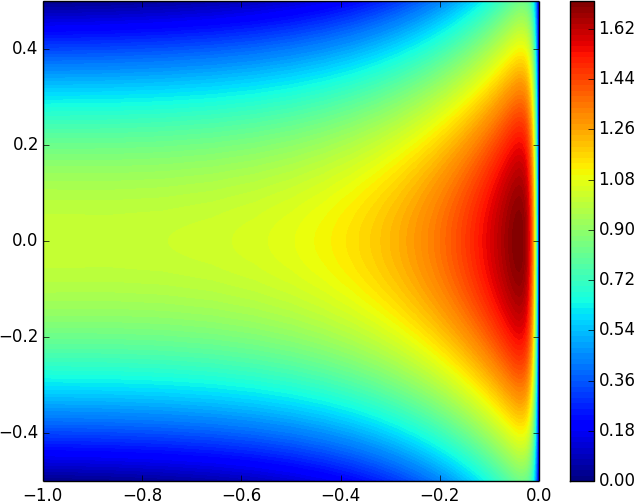
\includegraphics[width=\textwidth]{Confusion/Robustness/2d_problem_t_=_00.png}\\
$t=0.0$
\end{figure}
\end{column}
\begin{column}{0.3\textwidth}
\begin{figure}[t]
\centering
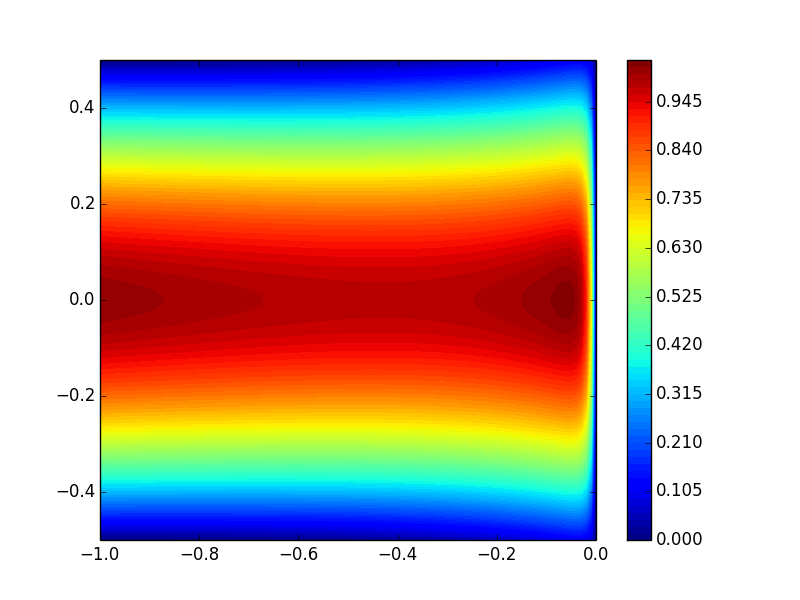
\includegraphics[width=\textwidth]{Confusion/Robustness/2d_problem_t_=_05.png}\\
$t=0.5$
\end{figure}
\end{column}
\begin{column}{0.3\textwidth}
\begin{figure}[t]
\centering
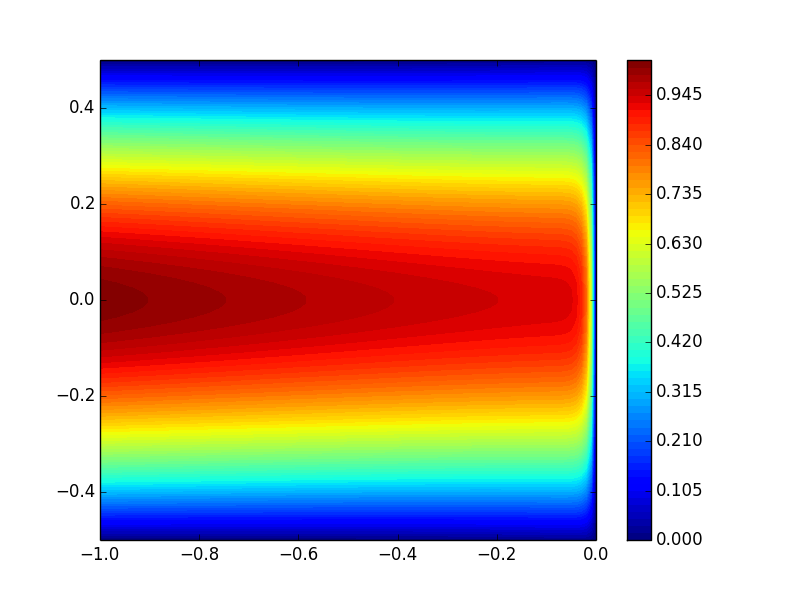
\includegraphics[width=\textwidth]{Confusion/Robustness/2d_problem_t_=_10.png}\\
$t=1.0$
\end{figure}
\end{column}
\end{columns}
\end{frame}

% ------------------------------------------------------------
\begin{frame}[t]
\frametitle{Robust Norms for Transient Convection-Diffusion}
\framesubtitle{Robust Convergence to Analytical Solution}
\vspace{-6.5ex}
\begin{columns}[t]
\begin{column}{0.4\textwidth}
\begin{figure}[t]
\centering
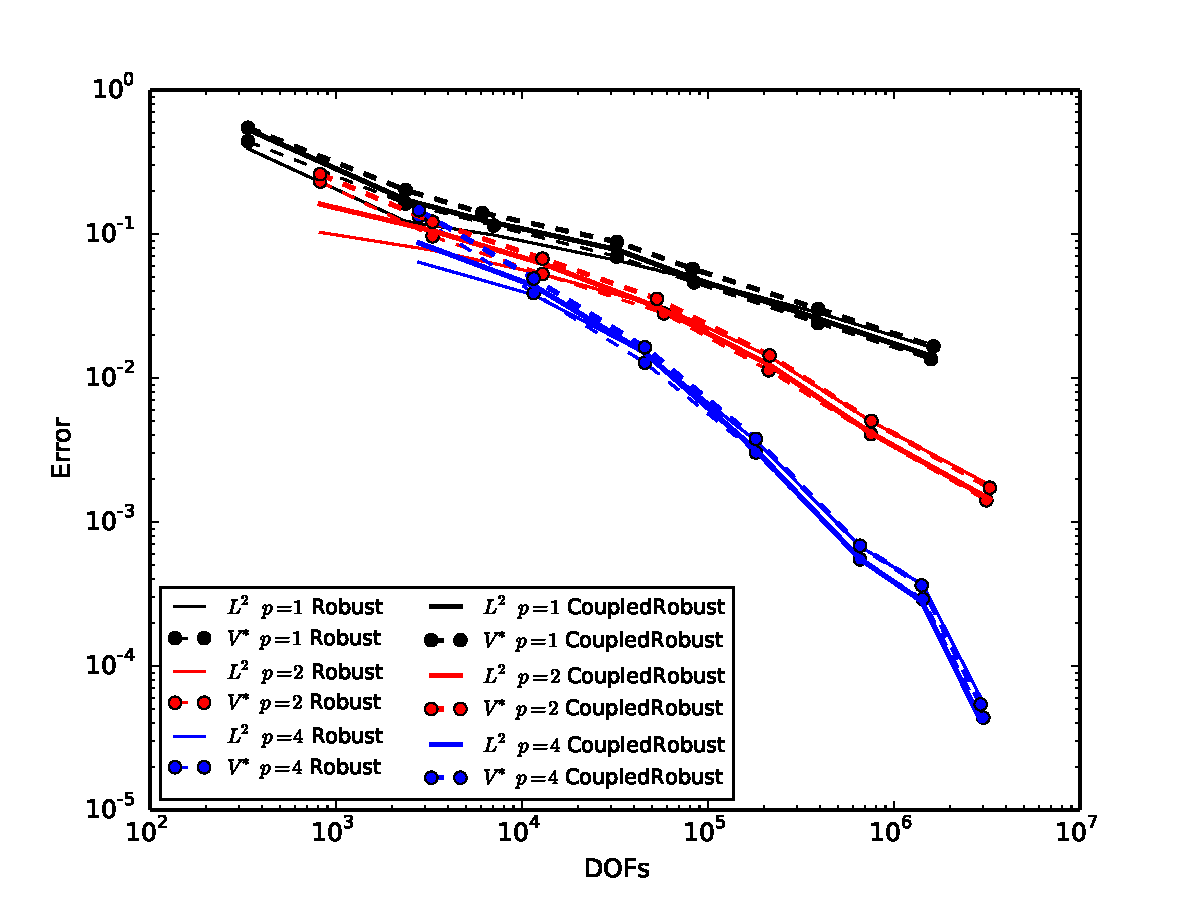
\includegraphics[width=\textwidth]{Confusion/Robustness/convergence_epsilon=1e-2.pdf}\\
\footnotesize{$\epsilon=10^{-2}$}\\
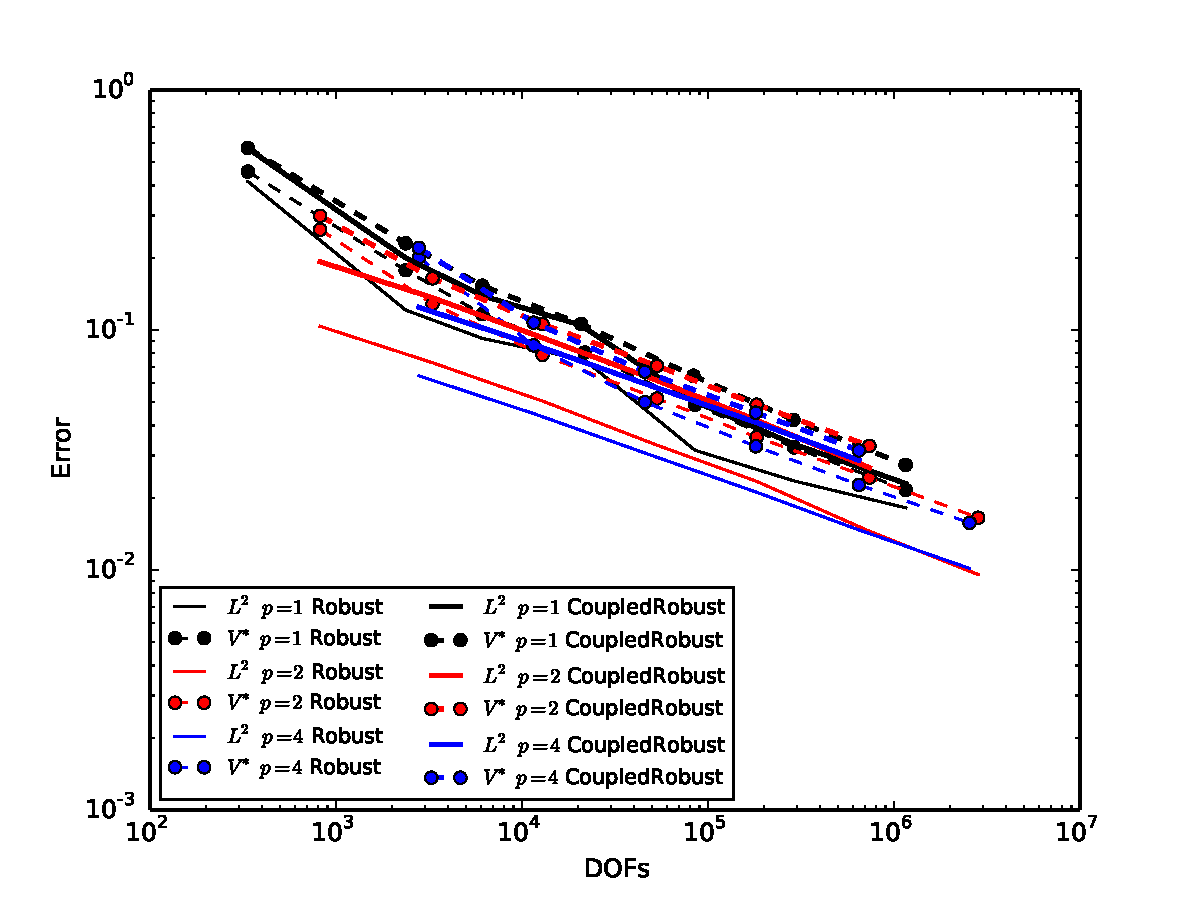
\includegraphics[width=\textwidth]{Confusion/Robustness/convergence_epsilon=1e-6.pdf}\\
\footnotesize{$\epsilon=10^{-6}$}
\end{figure}
\end{column}
\begin{column}{0.4\textwidth}
\begin{figure}[t]
\centering
\includegraphics[width=\textwidth]{Confusion/Robustness/convergence_epsilon=1e-4.pdf}\\
\footnotesize{$\epsilon=10^{-4}$}\\
\includegraphics[width=\textwidth]{Confusion/Robustness/convergence_epsilon=1e-8.pdf}\\
\footnotesize{$\epsilon=10^{-8}$}
\end{figure}
\end{column}
\end{columns}
\end{frame}



\section{Space-Time Incompressible Navier-Stokes}
% ------------------------------------------------------------
\begin{frame}[t]
\frametitle{Space-Time Incompressible Navier-Stokes}
\framesubtitle{Nonlinear Form}
Space-time divergence form:
\begin{align*}
  \frac{1}{\nu}\bbD-\Grad\bfu&=0\\
  \Divxt\vecttwo{\bfu\otimes\bfu-\bbD+p\bbI}{\bfu}&=\bff\\
  \Div\bfu&=0
\end{align*}
Multiply by $\bbS\in\bbH(\text{div},Q)$, $\bfv\in\bfH^1_{xt}(Q)$, $q\in\HonexQ$, 
and integrate by parts:
\begin{align*}
  \LRp{\frac{1}{\nu}\bbD,\bbS}
  +\LRp{\bfu,\Div\bbS}
  -\LRa{\hat\bfu,\bbS\cdot\bfn_x}&=0\\
  -\LRp{\vecttwo{\bfu\otimes\bfu-\bbD+p\bbI}{\bfu},\Gradxt\bfv}
  +\LRa{\hat\bft,\bfv}
  &=(\bff,\bfv)\\
  -\LRp{\bfu,\Grad q}
  +\LRa{\hat{\bfu}\cdot\bfn,q}&=0
\end{align*}
\end{frame}



% ------------------------------------------------------------
\begin{frame}[t]
\frametitle{Space-Time Incompressible Navier-Stokes}
\framesubtitle{Robust Norms}
Recall the adjoint and robust norm for convection-diffusion:
\begin{equation*}
  (\bfsigma,\frac{1}{\epsilon}\bftau+\Grad v)+(u,\Div\bftau-\bfbeta\cdot\Grad v-\pd{v}{t})
\end{equation*}
\begin{align*}
\norm{\LRp{v,\bftau}}_{V,K}^2 &\coloneqq
\norm{\bfbeta\cdot\Grad v+\pd{v}{t}}_K^2
+ \epsilon\norm{\Grad v}_K^2
+ \min\LRp{\frac{\epsilon}{h^2},1}\norm{v}^2_K
\\\nonumber&\quad
+ \norm{\Div \bftau}_K^2
+ \min\LRp{\frac{1}{\epsilon},\frac{1}{h^2}}\norm{\bftau}_K^2
\end{align*}
For incompressible Navier-Stokes the adjoint comes from:
\begin{align*}
  \LRp{\Delta\bbD,\frac{1}{\nu}\bbS+\Grad\bfv}
  &+\LRp{\Delta\bfu,\Div\bbS-\Grad q-\LRp{\tilde\bfu\cdot\Grad\bfv +\tilde\bfu\cdot(\Grad\bfv)^T+\pd{\bfv}{t}}}
  \\&+\LRp{p,-\Div\bfv}
\end{align*}
\end{frame}



% ------------------------------------------------------------
\begin{frame}[t]
\frametitle{Space-Time Incompressible Navier-Stokes}
\framesubtitle{~}
\vspace{-2ex}
\begin{block}{Norms for Navier-Stokes come from analogy}
\centering
\begin{tabular}{rcl}
Convection-Diffusion & & Navier-Stokes\\
$\epsilon$ &$\rightarrow$& $\nu$ \\
$\bftau$ &$\rightarrow$& $\bbS$ \\
$\Grad v$ &$\rightarrow$& $\Grad\bfv$ \\
$\Div\bftau$ &$\rightarrow$& $\Div\bbS-\Grad q$ \\
$\bfbeta\cdot\Grad v+\pd{v}{t}$ &$\rightarrow$& $\tilde\bfu\cdot\Grad\bfv+\tilde\bfu\cdot(\Grad\bfv)^T+\pd{\bfv}{t}$
\end{tabular}
\end{block}
\vspace{-1ex}
\begin{columns}
\begin{column}{0.2\textwidth}
Robust norm: 
\end{column}
\begin{column}{0.8\textwidth}
\begin{align*}
\norm{\LRp{\bfv,\bbD,q}}_{V,K}^2 &\coloneqq
\norm{\tilde\bfu\cdot\Grad\bfv +\tilde\bfu\cdot(\Grad\bfv)^T+\pd{\bfv}{t}}_K^2
+ \nu\norm{\Grad\bfv}_K^2
\\&\quad
+ \min\LRp{\frac{\nu}{h^2},1}\norm{\bfv}^2_K
+ \norm{\Div\bbS-\Grad q}_K^2
\\\nonumber&\quad
+ \min\LRp{\frac{1}{\nu},\frac{1}{h^2}}\norm{\bbS}_K^2
+\norm{\Div\bfv}_K^2
+\norm{q}_K^2
\end{align*}
\end{column}
\end{columns}
\end{frame}



% ------------------------------------------------------------
\begin{frame}[t]
\frametitle{Space-Time Incompressible Navier-Stokes}
\framesubtitle{Taylor-Green Vortex}
\vspace{-7ex}
\begin{columns}
\begin{column}{0.4\textwidth}
\[
\bfu=e^{-\frac{2}{Re}t}\vecttwo{\sin{x}\cos{y}}{-\cos{x}\sin{y}}
\]
\begin{figure}
\centering
\includegraphics[width=\textwidth]{Incompressible/TaylorGreen/Taylor-Green_vortex_vector_plot.png}
\end{figure}
\end{column}
\begin{column}{0.6\textwidth}
\begin{figure}
\centering
\includegraphics[width=\textwidth]{Incompressible/TaylorGreen/coupledrobust_convergence.pdf}
\end{figure}
\end{column}
\end{columns}
\end{frame}



\section{Space-Time Compressible Navier-Stokes}
% ------------------------------------------------------------
\begin{frame}[t]
\frametitle{Space-Time Compressible Navier-Stokes}
\framesubtitle{First Order System with Primitive Variables}
Assuming Stokes hypothesis, ideal gas law, and constant viscosity:
\begin{align*}
  \frac{1}{\mu}\mathbb{D}-\Grad\bfu&=0\\
  \frac{Pr}{C_p\mu}\bfq+\Grad T&=0\\
  \Divxt\vecttwo{\rho\bfu}{\rho}&=f_c\\
  \Divxt\vecttwo{\rho\bfu\otimes\bfu+\rho RT\bbI-\LRp{\bbD+\bbD^T-\frac{2}{3}\trace(\bbD)\bbI}}{\rho\bfu}&=\bff_m\\
  \Divxt\vecttwo{\rho\bfu\LRp{C_v T+\frac{1}{2}\bfu\cdot\bfu}+\rho RT\bfu+\bfq-\bfu\cdot\LRp{\bbD+\bbD^T-\frac{2}{3}\trace(\bbD)\bbI}}{\rho\LRp{C_v T+\frac{1}{2}\bfu\cdot\bfu}}&=f_e
\end{align*}
\end{frame}


% ------------------------------------------------------------
\begin{frame}[t]
\frametitle{Space-Time Compressible Navier-Stokes}
\framesubtitle{Compact Notation}
\begin{columns}[t]
\begin{column}{0.5\textwidth}
Conserved quantities
\vspace{-2ex}
\begin{align*}
C_c&:=\rho\\
\bfC_m&:=\rho\bfu\\
C_e&:=\rho(C_v T+\frac{1}{2}\bfu\cdot\bfu)\\
% C&:=\LRc{C_c\,,\, \bfC_m\,,\, C_e}\\
\end{align*}
\end{column} 
\begin{column}{0.5\textwidth}
Euler fluxes 
\vspace{-2ex}
\begin{align*}
\bfF_c&:=\rho\bfu\\
\bbF_m&:=\rho\bfu\otimes\bfu+\rho RT\bbI\\
\bfF_e&:=\rho\bfu\LRp{C_v T+\frac{1}{2}\bfu\cdot\bfu}+\rho RT\bfu\\
% F&:=\LRc{\bfF_c\,,\, \bbF_m\,,\, \bfF_e}\\
\end{align*}
\end{column} 
\end{columns}
\begin{columns}[t]
\begin{column}{0.3\textwidth}
Viscous fluxes 
\vspace{-2ex}
\begin{align*}
\bfK_c&:=\boldsymbol 0\\
\bbK_m&:=\bbD+\bbD^T-\frac{2}{3}\trace(\bbD)\bbI\\
\bfK_e&:=-\bfq+\bfu\cdot\LRp{\bbD+\bbD^T-\frac{2}{3}\trace(\bbD)\bbI}\\
% K&:=\LRc{\bfK_c\,,\, \bbK_m\,,\, \bfK_e}\\
\end{align*}
\end{column} 
\begin{column}{0.3\textwidth}
Viscous variables
\vspace{-2ex}
\begin{align*}
\bbM_{\bbD}&:=\bbD\\
\bfM_{\bfq}&:=\frac{Pr}{C_p}\bfq\\
% M&:=\LRc{\bbM_{\bbD}\,,\, \bfM_{\bfq}}\\
\bfG_{\bbD}&:=2\bfu\\
G_{\bfq}&:=-T\\
% G&:=\LRc{\bfG_{\bbD}\,,\, G_{\bfq}}\\
\end{align*}
\end{column} 
\end{columns}
\centering
Use change of variables to get conservation or entropy variables.
% \begin{align*}
% f&:=\LRc{f_c\,,\, \bff_m\,,\, f_e}\\
% \end{align*}
% and group variables
% \begin{align*}
% W&:=\LRc{\rho\,,\,\bfu\,,\,T}\\
% \hat W&:=\LRc{2\hat\bfu\,,\,-\hat T}\\
% \Sigma&:=\LRc{\bbD,\bfq}\\
% \hat t&:=\LRc{\hat t_e\,,\,\hat\bft_m,\,,\,\hat t_e}\\
% \Psi&:=\LRc{\bbS\,,\,\bftau}\\
% V&:=\LRc{v_c\,,\,\bfv_m,\,,\,v_e}\,.
% \end{align*}
\end{frame}


% ------------------------------------------------------------
\begin{frame}[t]
\frametitle{Space-Time Compressible Navier-Stokes}
\framesubtitle{Conservation Variables (Popular for Time-Stepping)}
% \begin{columns}[t]
% \begin{column}{0.5\textwidth}
% Now we wish to do a change of variables to conservation variables: 
Change of variables:
\begin{align*}
\rho&=\rho\\
\bfm&=\rho\bfu\\
E&=\rho\LRp{C_v T+\frac{1}{2}\bfu\cdot\bfu}
\end{align*}
Euler fluxes:
\begin{align*}
\bfF^c_c&=\bfm\\
\mathbb{F}^c_m&=\frac{\bfm\otimes\bfm}{\rho}+(\gamma-1)\LRp{E-\frac{\bfm\cdot\bfm}{2\rho}}\bbI\\
\bfF^c_e&=\gamma E\frac{\bfm}{\rho}-(\gamma-1)\frac{\bfm\cdot\bfm}{2\rho^2}\bfm\\
\end{align*}
% \end{column}
% \begin{column}{0.5\textwidth}
% \end{column}
% \end{columns}
\end{frame}


% ------------------------------------------------------------
\begin{frame}[t]
\frametitle{Space-Time Compressible Navier-Stokes}
\framesubtitle{Entropy Variables (Symmetrize the Bubnov-Galerkin Stiffness Matrix)}
% \vspace{-4ex}
Change of variables:

\scalebox{0.78}{\parbox{\linewidth}{%
\begin{align*}
V_c&=\frac{-E+(E-\frac{1}{2\rho}\bfm\cdot\bfm)\LRp{\gamma+1-\ln\LRs{\frac{(\gamma-1)(E-\frac{1}{2\rho}\bfm\cdot\bfm)}{\rho^\gamma}}}}
{E-\frac{1}{2\rho}\bfm\cdot\bfm}\\
\bfV_m&=\frac{\bfm}{E-\frac{1}{2\rho}\bfm\cdot\bfm}\\
V_e&=\frac{-\rho}{E-\frac{1}{2\rho}\bfm\cdot\bfm}
\end{align*}
}}

% with reverse mapping:
% \begin{align*}
% \rho&=-\alpha V_e\\
% \bfm&=\alpha\bfV_m\\
% E&=\alpha\LRp{1-\frac{1}{2V_e}\bfV_m\cdot\bfV_m}\\
% \end{align*}
% We can define new fluxes in entropy variables:
% \bfF^e_c&=\alpha\bfV_m\\
% \mathbb{F}^e_m&=\alpha\LRp{-\frac{\bfV_m\otimes\bfV_m}{V_e}+(\gamma-1)\bbI}\\
% \bfF^e_e&=\alpha\frac{\bfV_m}{V_e}\LRp{\frac{1}{2V_e}\bfV_m\cdot\bfV_m-\gamma}\\
Euler fluxes:

\scalebox{0.78}{\parbox{\linewidth}{%
\begin{align*}
\bfF^e_c&=\LRs{\frac{\gamma-1}{(-V_e)^\gamma}}^{\frac{1}{\gamma-1}}\exp\LRs{\frac{-\gamma+V_c-\frac{1}{2V_e}\bfV_m\cdot\bfV_m}{\gamma-1}}\bfV_m\\
\mathbb{F}^e_m&=\LRs{\frac{\gamma-1}{(-V_e)^\gamma}}^{\frac{1}{\gamma-1}}\exp\LRs{\frac{-\gamma+V_c-\frac{1}{2V_e}\bfV_m\cdot\bfV_m}{\gamma-1}}\LRp{-\frac{\bfV_m\otimes\bfV_m}{V_e}+(\gamma-1)\bbI}\\
\bfF^e_e&=\LRs{\frac{\gamma-1}{(-V_e)^\gamma}}^{\frac{1}{\gamma-1}}\exp\LRs{\frac{-\gamma+V_c-\frac{1}{2V_e}\bfV_m\cdot\bfV_m}{\gamma-1}}\frac{\bfV_m}{V_e}\LRp{\frac{1}{2V_e}\bfV_m\cdot\bfV_m-\gamma}
\end{align*}
}}
% where 
% \[
% \alpha(V_c,\bfV_m,V_e)=\LRs{\frac{\gamma-1}{(-V_e)^\gamma}}^{\frac{1}{\gamma-1}}\exp\LRs{\frac{-\gamma+V_c-\frac{1}{2V_e}\bfV_m\cdot\bfV_m}{\gamma-1}}
% \]
% \end{column}
% \end{columns}
\end{frame}


% ------------------------------------------------------------
\begin{frame}[t]
\frametitle{Space-Time Compressible Navier-Stokes}
\framesubtitle{Define Group Variables}
\begin{columns}[t]
\begin{column}{0.5\textwidth}
Group terms
\vspace{-2ex}
\begin{align*}
C&:=\LRc{C_c\,,\, \bfC_m\,,\, C_e}\\
F&:=\LRc{\bfF_c\,,\, \bbF_m\,,\, \bfF_e}\\
K&:=\LRc{\bfK_c\,,\, \bbK_m\,,\, \bfK_e}\\
M&:=\LRc{\bbM_{\bbD}\,,\, \bfM_{\bfq}}\\
G&:=\LRc{\bfG_{\bbD}\,,\, G_{\bfq}}\\
f&:=\LRc{f_c\,,\, \bff_m\,,\, f_e}\\
\end{align*}
\end{column}
\begin{column}{0.5\textwidth}
Group variables
\vspace{-2ex}
\begin{align*}
W&:=\LRc{\rho\,,\,\bfu\,,\,T}\\
\hat W&:=\LRc{2\hat\bfu\,,\,-\hat T}\\
\Sigma&:=\LRc{\bbD,\bfq}\\
\hat t&:=\LRc{\hat t_e\,,\,\hat\bft_m,\,,\,\hat t_e}\\
\Psi&:=\LRc{\bbS\,,\,\bftau}\\
V&:=\LRc{v_c\,,\,\bfv_m,\,,\,v_e}
\end{align*}
\end{column}
\end{columns}
Navier-Stokes variational formulation is
\begin{align*}
\LRp{\frac{1}{\mu}M,\Psi}+\LRp{G,\Div\Psi}-\LRa{\hat W,\Psi\cdot\bfn_x}&=0\\
-\LRp{\vecttwo{F-K}{C},\Gradxt V}+\LRa{\hat t,V}&=\LRp{f,V}
\end{align*}
\end{frame}




%    /$$$$$$                  /$$
%   /$$__  $$                | $$
%  | $$  \__/  /$$$$$$   /$$$$$$$
%  |  $$$$$$  /$$__  $$ /$$__  $$
%   \____  $$| $$  \ $$| $$  | $$
%   /$$  \ $$| $$  | $$| $$  | $$
%  |  $$$$$$/|  $$$$$$/|  $$$$$$$
%   \______/  \______/  \_______/
%                                
%                                
%        
% ------------------------------------------------------------
\begin{frame}[t]
\frametitle{Space-Time Compressible Navier-Stokes}
\framesubtitle{Sod Shock Tube with $\mu=10^{-5}$}  %% needed for proper positioning of the logo ...
\foreach \n in {1,...,15}
{
\only<\n>
{
\vspace{-2ex}
\begin{figure}[ht]
\centering

% \begin{subfigure}[c]{0.45\textwidth}
% \centering
% \includegraphics[height=0.7\textwidth]{Sod/FormulationComparison/den\n.pdf}
% \end{subfigure}
% \begin{subfigure}[c]{0.45\textwidth}
% \centering
% \includegraphics[height=0.7\textwidth]{Sod/FormulationComparison/vel\n.pdf}
% \end{subfigure}
% \begin{subfigure}[c]{0.45\textwidth}
% \centering
% \includegraphics[height=0.7\textwidth]{Sod/FormulationComparison/pres\n.pdf}
% \end{subfigure}
\textcolor{utblack}{Mesh \n}\\
\vspace{1ex}
\begin{subfigure}[c]{0.65\textwidth}
\centering
\includegraphics[width=1.0\textwidth]{Sod/FormulationComparison/Form0Mesh\n.png}\\
Primitive Variables\\
\vspace{2ex}
\end{subfigure}
\begin{subfigure}[c]{0.65\textwidth}
\centering
\includegraphics[width=1.0\textwidth]{Sod/FormulationComparison/Form1Mesh\n.png}\\
Conservation Variables\\
\vspace{2ex}
\end{subfigure}
\begin{subfigure}[c]{0.65\textwidth}
\centering
\includegraphics[width=1.0\textwidth]{Sod/FormulationComparison/Form2Mesh\n.png}\\
Entropy Variables\\
\end{subfigure}
\end{figure}
}
}
\end{frame}

\begin{frame}[t]
\frametitle{Space-Time Compressible Navier-Stokes}
\framesubtitle{Sod Shock Tube with $\mu=10^{-5}$}  %% needed for proper positioning of the logo ...
\foreach \n in {1,...,15}
{
\only<\n>
{
\vspace{-2ex}
\begin{figure}[ht]
\centering

\begin{subfigure}[c]{0.45\textwidth}
\centering
\includegraphics[height=0.7\textwidth]{Sod/FormulationComparison/den\n.pdf}
\end{subfigure}
\begin{subfigure}[c]{0.45\textwidth}
\centering
\includegraphics[height=0.7\textwidth]{Sod/FormulationComparison/vel\n.pdf}
\end{subfigure}
\begin{subfigure}[c]{0.45\textwidth}
\centering
\includegraphics[height=0.7\textwidth]{Sod/FormulationComparison/pres\n.pdf}
\end{subfigure}
% \begin{subfigure}[c]{0.45\textwidth}
% \centering
% \includegraphics[width=1.0\textwidth]{Sod/FormulationComparison/mesh\n.png}
% \end{subfigure}
\end{figure}
}
}
\end{frame}


% ------------------------------------------------------------
\begin{frame}[t]
\frametitle{Space-Time Compressible Navier-Stokes}
\framesubtitle{Entropy Scaled Test Norms}  %% needed for proper positioning of the logo ...
Let $W$, $U$, and $V$ be the set of primitive, conservation, and entropy variables.

The entropy function
\[
H=-\rho\log(p\rho^{-\gamma})
\]
provides a natural residual for the Navier-Stokes equations.

$A_0=H_{,UU}=V_{,U}$
is known as the symmetrizer and $(U,A_0U)$ provides a natural metric for the Euler equations.

In primitive variables: 
\[
(u,A_0U)=(U_{,W}W,V_{,U}U_{,W}W)=(W,U_{,W}^TV_{,U}U_{,W}W)=(W,A_0(W)W)
\]
where
\[
A_0(W)=U_{,W}^TV_{,U}U_{,W}=\arrthree
{\frac{\gamma-1}{\rho}}
{0}
{0}
{0}
{\frac{\rho}{C_v T}}
{0}
{0}
{0}
{\frac{\rho}{T^2}}
\]

\end{frame}


% ------------------------------------------------------------
\begin{frame}[t]
\frametitle{Space-Time Compressible Navier-Stokes}
\framesubtitle{Entropy Scaled Test Norms}  %% needed for proper positioning of the logo ...
Bilinear form with group variables:
\[
b\LRp{\LRp{W,\hat W},v} = \LRp{W,A^*_h v}_{\LOmega} + \LRa{\hat W, \jump{v}}_{\Gh}
\]
For conforming $v^*$ satisfying $A^* v^* = A_0W$
\begin{align*}
&\norm{A_0^\frac{1}{2}W}^2
=\frac{b(W,v^*)}{\norm{v^*}_V} \norm{v^*}_V\\
&\quad\leq\sup_{v^*\neq0}\frac{|b(W,v^*)|}{\norm{v^*}}\norm{v^*}
=\norm{W}_E \norm{v^*}_V\,.
\end{align*}
Necessary robustness condition:
\begin{align*}
&\norm{v^*}_V\lesssim\norm{A_0^\frac{1}{2}W}_{L^2(\Omega_h)}\\
&\quad\Rightarrow\norm{A_0^\frac{1}{2}W}_{L^2(\Omega_h)}\lesssim\norm{W}_E
\end{align*}
\end{frame}


% ------------------------------------------------------------
\begin{frame}[t]
\frametitle{Space-Time Compressible Navier-Stokes}
\framesubtitle{Entropy Scaled Test Norms}  %% needed for proper positioning of the logo ...
We load our adjoint equations with $A_0W$:
\begin{align*}
\frac{1}{\mu}M^*(\Psi)+K^*(\Grad V)&=0
\\
-\vecttwo{F^*}{C^*}(\Gradxt V)+G^*(\Grad\Psi)&=A_0W
\end{align*}
This leads to the entropy scaled robust norm:
\begin{align*}
\norm{\LRp{V,\Psi}}_{V,K}^2 &\coloneqq
\norm{A_0^{-\frac{1}{2}}(F^*+C^*)}_K^2
+ \mu\norm{A_0^{-\frac{1}{2}}K^*}_K^2
\\\nonumber&\quad
+ \min\LRp{\frac{\mu}{h^2},1}\norm{A_0^{-\frac{1}{2}}V}^2_K
+ \norm{A_0^{-\frac{1}{2}}G^*}_K^2
\\\nonumber&\quad
+ \min\LRp{\frac{1}{\mu},\frac{1}{h^2}}\norm{A_0^{-\frac{1}{2}}M^*}_K^2
\end{align*}
\uncover<2>{\textcolor{utorange}{Numerical results were disappointing.}}
\end{frame}



%   /$$   /$$           /$$      
%  | $$$ | $$          | $$      
%  | $$$$| $$  /$$$$$$ | $$$$$$$ 
%  | $$ $$ $$ /$$__  $$| $$__  $$
%  | $$  $$$$| $$  \ $$| $$  \ $$
%  | $$\  $$$| $$  | $$| $$  | $$
%  | $$ \  $$|  $$$$$$/| $$  | $$
%  |__/  \__/ \______/ |__/  |__/
%                                
%                                
% 
% ------------------------------------------------------------
\begin{frame}[t]
\frametitle{Space-Time Compressible Navier-Stokes}
\framesubtitle{Noh Implosion with Primitive Variables, Robust Norm, $\mu=10^{-3}$}  %% needed for proper positioning of the logo ...

\begin{columns}[t]
\begin{column}[c]{0.7\textwidth}
% Standard robust test norm with primitive variables
\centering
\includegraphics[width=1.05\textwidth]{Dissertation/Noh/Robust-den.pdf}
\end{column}
\begin{column}[c]{0.28\textwidth}
\centering
% \hspace{-2ex}\includegraphics[width=\textwidth]{Dissertation/Noh/Robust-mesh0.png}
% \\Initial Mesh
After 5 refinements\\
\hspace{-2ex}\includegraphics[width=\textwidth]{Dissertation/Noh/Robust-mesh5.png}
\\After 10 refinements
\\
\hspace{-2ex}\includegraphics[width=\textwidth]{Dissertation/Noh/Robust-mesh10.png}
\end{column}
\end{columns}

\end{frame}



% ------------------------------------------------------------
\begin{frame}[t]
\frametitle{Space-Time Compressible Navier-Stokes}
\framesubtitle{Piston with $\mu=10^{-2}$}  %% needed for proper positioning of the logo ...

\vspace{-2ex}
\begin{columns}[t]
\begin{column}[c]{0.7\textwidth}
% Left boundary:
\small
\begin{align*}
\hat t_c&=\sqrt{2}(-\rho u+\rho)\\
\hat t_m&=\sqrt{2}(-\rho u^2-\rho RT+\rho u)\\
\hat t_e&=\sqrt{2}(-\rho u(C_vT+\frac{1}{2}u^2)-u\rho RT+\rho(C_vT+\frac{1}{2}u^2))
\end{align*}
\end{column}
% \begin{column}[c]{0.25\textwidth}
% % and since $u=1$ at the left wall
% \small
% \begin{align*}
% \hat t_c&=0\\
% \hat t_m&=-\sqrt{2}\rho RT\\
% \hat t_e&=-\sqrt{2}\rho RT
% \end{align*}
% \end{column}
\begin{column}[c]{0.3\textwidth}
\small
\begin{align*}
\hat u&=1\\
\hat t_c&=0\\
\hat t_m - \hat t_e&=0
\end{align*}
\end{column}
\end{columns}

\begin{columns}[t]
\begin{column}[c]{0.5\textwidth}
\centering
\includegraphics[width=\textwidth]{Piston/Piston_density.png}
\\Density
\end{column}
\begin{column}[c]{0.5\textwidth}
\centering
\includegraphics[width=\textwidth]{Piston/Piston_velocity.png}
\\Velocity
\end{column}
\end{columns}
\end{frame}



% ------------------------------------------------------------
\begin{frame}[t]
\frametitle{Space-Time Compressible Navier-Stokes}
\framesubtitle{Piston with $\mu=10^{-2}$}  %% needed for proper positioning of the logo ...

\centering
\includegraphics[width=0.7\textwidth]{Piston/Piston_mesh.png}
\\Mesh after 8 adaptive refinements
\end{frame}



\begin{frame}[shrink=10]
\frametitle{Thank You!}
\framesubtitle{Recommended References}
    \nocite{DPGOverview}
    \nocite{EllisLC}
    \nocite{CamelliaDPG}
    \nocite{DemkowiczHeuer}
    \nocite{ChanHeuerThanhDemkowicz2012}
    \nocite{DPGStokes}
    \renewcommand*{\bibfont}{\small}
    \setbeamertemplate{bibliography item}[triangle]
    \printbibliography[keyword=main]
    % \bigskip
    \printbibliography[notkeyword=main]
\end{frame}

\appendix







\begin{frame}
\frametitle{Scaling Issues}
\framesubtitle{Multigrid and Convection-Diffusion}  %% needed for proper positioning of the logo ...
\begin{columns}
\begin{column}{0.4\textwidth}
\begin{itemize}
  \item Convection-diffusion, $\epsilon=10^{-2}$, $64\times64$ mesh
  \item Conjugate gradient
  \item Geometric multigrid preconditioner
  % \begin{itemize}
    \item Multiplicative V-cycle
    \item Overlapping additive Schwarz smoother
    \item Hierarchy of $p-$coarsening followed by $h-$coarsening
  % \end{itemize}
\end{itemize}
\end{column}
\begin{column}{0.6\textwidth}
\centering
\includegraphics[width=\textwidth]{Dissertation/Scaling/ConfusionResidual.pdf}
\end{column}
\end{columns}
\end{frame}



\begin{frame}
\frametitle{Scaling Issues}
\framesubtitle{Incompressible Flow Over a Cylinder, \only<1>{Initial Mesh}\only<2>{4 Refinements}}  %% needed for proper positioning of the logo ...
\begin{figure}
\centering
\only<1>{\includegraphics[width=0.8\textwidth]{Dissertation/Cylinder/Mesh_uMag0.png}}
\only<2>{\includegraphics[width=0.8\textwidth]{Dissertation/Cylinder/Mesh_uMag4.png}}
\end{figure}
\end{frame}



\begin{frame}
\frametitle{Scaling Issues}
\framesubtitle{Solve Times and Strong Scaling}  %% needed for proper positioning of the logo ...
\begin{block}{Transient Flow Over a Cylinder}
\resizebox{0.95\linewidth}{!}{
\begin{minipage}{\linewidth}
\begin{table}[!ht]
\centering
\begin{tabular}{|crr|r|rc|rc|}
\hline
& & & 1 Node & \multicolumn{2}{|c|}{4 Nodes} & \multicolumn{2}{|c|}{32 Nodes} \\
Ref& Elems & DOFs & Time    & Time & Scaling vs 1     & Time & Scaling vs 4      \\
\hline
0 & 80            & 31304      & 1772   & 453   & 3.91 & 451  & 1.01 \\
1 & 605           & 225908     & 8190   & 3574  & 2.29 & 717  & 4.98 \\
2 & 3013          & 1081598    & 32008  & 12076 & 2.65 & 2648 & 4.56 \\
3 & 9726          & 3429384    &          & 28744 &      & 6319 & 4.54 \\
4 & 11742         & 4144674    &          &         &      & 8510 &      \\
\hline
% & & & 8.8 hours & 8.0 hours & & 2.4 hours &
\end{tabular}
\end{table}
\end{minipage}
}
\end{block}
Computations on Lonestar, 1 node = 24 processors

32008 seconds = 8.8 hours\\ 28744 seconds = 8.0 hours\\ \hspace{1ex}8510 seconds = 2.4 hours
\end{frame}



\begin{frame}
\frametitle{Scaling Issues}
\framesubtitle{Solve Times and Strong Scaling}  %% needed for proper positioning of the logo ...
\begin{block}{Taylor-Green Vortex}
\begin{table}[!ht]
\centering
\begin{tabular}{|crr|r|rc|}
\hline
& & & 1 Node & \multicolumn{2}{|c|}{4 Nodes} \\
Ref& Elems & DOFs & Time    & Time & Scaling vs 1 \\
\hline
0 & 60            & 21302      & 331    & 140   & 2.35 \\
1 & 312           & 108410     & 945    & 290   & 3.25 \\
2 & 2020          & 691834     & 4880   & 1363  & 3.58 \\
3 & 9244          & 3043024    &        & 6171  & \\
\hline
\end{tabular}
\end{table}
\end{block}
Computations on Lonestar, 1 node = 24 processors

4880 seconds = 1.4 hours\\
6171 seconds = 1.7 hours
\end{frame}



\begin{frame}
\frametitle{Scaling Issues}
\framesubtitle{Space-Time Slabs}  %% needed for proper positioning of the logo ...
Assumptions:
\begin{itemize}
\item The maximum required spatial resolution is much finer than the required temporal resolution.
\item Regions requiring high spatial resolution are concentrated in relatively compact parts of the domain.
\item Only isotropic refinements are permitted.
\item The number of time slabs is a power of 2.
\end{itemize}
Test problem: convection diffusion with exact solution
\[
u=1-e^\frac{x}{\epsilon}
\]
on space-time domain $[-1,0]\times[0,1]$.
\end{frame}



\begin{frame}
\frametitle{Scaling Issues}
\framesubtitle{Space-Time Slabs}  %% needed for proper positioning of the logo ...
\begin{figure}
\centering
\begin{tikzpicture}[line cap=round,line join=round,>=triangle 45,x=10cm,y=10cm, scale=0.5, every node/.style={scale=0.5}]
% \clip(-0.7,-0.6) rectangle (5.27,2.09);
% horizontal
\draw (0,0)-- (1,0);
\draw (0,1)-- (1,1);
% vertical
\draw (0,0)-- (0,1);
\draw (1,0)-- (1,1);

% horizontal
\draw (0,.5)-- (1,.5);
%vertical
\draw (.5,0)-- (.5,1);

% horizontal
\draw (.5,.25)-- (1,.25);
\draw (.5,.75)-- (1,.75);
%vertical
\draw (.75,0)-- (.75,1);

% horizontal
\draw (.75,1/8)-- (1,1/8);
\draw (.75,3/8)-- (1,3/8);
\draw (.75,5/8)-- (1,5/8);
\draw (.75,7/8)-- (1,7/8);
%vertical
\draw (1-1/8,0)-- (1-1/8,1);

% horizontal
\draw (1-1/8,1/16)-- (1,1/16);
\draw (1-1/8,3/16)-- (1,3/16);
\draw (1-1/8,5/16)-- (1,5/16);
\draw (1-1/8,7/16)-- (1,7/16);
\draw (1-1/8,9/16)-- (1,9/16);
\draw (1-1/8,11/16)-- (1,11/16);
\draw (1-1/8,13/16)-- (1,13/16);
\draw (1-1/8,15/16)-- (1,15/16);
%vertical
\draw (1-1/16,0)-- (1-1/16,1);

\draw [->] (-0.125,-0.125) -- (-0.125,0);
\draw [->] (-0.125,-0.125) -- (0,-0.125);
\draw (-0.135,0.0725) node[anchor=north west] {$t$};
\draw (0.0175,-0.0875) node[anchor=north west] {$x$};
\end{tikzpicture}
\\Single Slab Strategy
% \label{fig:SingleSlab}
\end{figure}
\end{frame}


\begin{frame}
\frametitle{Scaling Issues}
\framesubtitle{Space-Time Slabs}  %% needed for proper positioning of the logo ...
\begin{figure}
\centering
\begin{tikzpicture}[line cap=round,line join=round,>=triangle 45,x=10cm,y=10cm, scale=0.5, every node/.style={scale=0.5}]
% \clip(-0.7,-0.6) rectangle (5.27,2.09);
% Slab 4
% horizontal
\draw (0,0+3/4+3/32)-- (1,0+3/4+3/32);
\draw (0,1/4+3/4+3/32)-- (1,1/4+3/4+3/32);
% vertical
\draw (0,0+3/4+3/32)-- (0,1/4+3/4+3/32);
\draw (1,0+3/4+3/32)-- (1,1/4+3/4+3/32);

% horizontal
\draw (0,1/8+3/4+3/32)-- (1,1/8+3/4+3/32);
%vertical
\draw (.5,0+3/4+3/32)-- (.5,1/4+3/4+3/32);

% horizontal
\draw (.5,1/16+3/4+3/32)-- (1,1/16+3/4+3/32);
\draw (.5,3/16+3/4+3/32)-- (1,3/16+3/4+3/32);
%vertical
\draw (.75,0+3/4+3/32)-- (.75,1/4+3/4+3/32);

% horizontal
\draw (.75,1/32+3/4+3/32)-- (1,1/32+3/4+3/32);
\draw (.75,3/32+3/4+3/32)-- (1,3/32+3/4+3/32);
\draw (.75,5/32+3/4+3/32)-- (1,5/32+3/4+3/32);
\draw (.75,7/32+3/4+3/32)-- (1,7/32+3/4+3/32);
%vertical
\draw (1-1/8,0+3/4+3/32)-- (1-1/8,1/4+3/4+3/32);

% horizontal
\draw (1-1/8,1/64+3/4+3/32)-- (1,1/64+3/4+3/32);
\draw (1-1/8,3/64+3/4+3/32)-- (1,3/64+3/4+3/32);
\draw (1-1/8,5/64+3/4+3/32)-- (1,5/64+3/4+3/32);
\draw (1-1/8,7/64+3/4+3/32)-- (1,7/64+3/4+3/32);
\draw (1-1/8,9/64+3/4+3/32)-- (1,9/64+3/4+3/32);
\draw (1-1/8,11/64+3/4+3/32)-- (1,11/64+3/4+3/32);
\draw (1-1/8,13/64+3/4+3/32)-- (1,13/64+3/4+3/32);
\draw (1-1/8,15/64+3/4+3/32)-- (1,15/64+3/4+3/32);
%vertical
\draw (1-1/16,0+3/4+3/32)-- (1-1/16,1/4+3/4+3/32);

% Slab 3
% horizontal
\draw (0,0+2/4+2/32)-- (1,0+2/4+2/32);
\draw (0,1/4+2/4+2/32)-- (1,1/4+2/4+2/32);
% vertical
\draw (0,0+2/4+2/32)-- (0,1/4+2/4+2/32);
\draw (1,0+2/4+2/32)-- (1,1/4+2/4+2/32);

% horizontal
\draw (0,1/8+2/4+2/32)-- (1,1/8+2/4+2/32);
%vertical
\draw (.5,0+2/4+2/32)-- (.5,1/4+2/4+2/32);

% horizontal
\draw (.5,1/16+2/4+2/32)-- (1,1/16+2/4+2/32);
\draw (.5,3/16+2/4+2/32)-- (1,3/16+2/4+2/32);
%vertical
\draw (.75,0+2/4+2/32)-- (.75,1/4+2/4+2/32);

% horizontal
\draw (.75,1/32+2/4+2/32)-- (1,1/32+2/4+2/32);
\draw (.75,3/32+2/4+2/32)-- (1,3/32+2/4+2/32);
\draw (.75,5/32+2/4+2/32)-- (1,5/32+2/4+2/32);
\draw (.75,7/32+2/4+2/32)-- (1,7/32+2/4+2/32);
%vertical
\draw (1-1/8,0+2/4+2/32)-- (1-1/8,1/4+2/4+2/32);

% horizontal
\draw (1-1/8,1/64+2/4+2/32)-- (1,1/64+2/4+2/32);
\draw (1-1/8,3/64+2/4+2/32)-- (1,3/64+2/4+2/32);
\draw (1-1/8,5/64+2/4+2/32)-- (1,5/64+2/4+2/32);
\draw (1-1/8,7/64+2/4+2/32)-- (1,7/64+2/4+2/32);
\draw (1-1/8,9/64+2/4+2/32)-- (1,9/64+2/4+2/32);
\draw (1-1/8,11/64+2/4+2/32)-- (1,11/64+2/4+2/32);
\draw (1-1/8,13/64+2/4+2/32)-- (1,13/64+2/4+2/32);
\draw (1-1/8,15/64+2/4+2/32)-- (1,15/64+2/4+2/32);
%vertical
\draw (1-1/16,0+2/4+2/32)-- (1-1/16,1/4+2/4+2/32);

% Slab 2
% horizontal
\draw (0,0+1/4+1/32)-- (1,0+1/4+1/32);
\draw (0,1/4+1/4+1/32)-- (1,1/4+1/4+1/32);
% vertical
\draw (0,0+1/4+1/32)-- (0,1/4+1/4+1/32);
\draw (1,0+1/4+1/32)-- (1,1/4+1/4+1/32);

% horizontal
\draw (0,1/8+1/4+1/32)-- (1,1/8+1/4+1/32);
%vertical
\draw (.5,0+1/4+1/32)-- (.5,1/4+1/4+1/32);

% horizontal
\draw (.5,1/16+1/4+1/32)-- (1,1/16+1/4+1/32);
\draw (.5,3/16+1/4+1/32)-- (1,3/16+1/4+1/32);
%vertical
\draw (.75,0+1/4+1/32)-- (.75,1/4+1/4+1/32);

% horizontal
\draw (.75,1/32+1/4+1/32)-- (1,1/32+1/4+1/32);
\draw (.75,3/32+1/4+1/32)-- (1,3/32+1/4+1/32);
\draw (.75,5/32+1/4+1/32)-- (1,5/32+1/4+1/32);
\draw (.75,7/32+1/4+1/32)-- (1,7/32+1/4+1/32);
%vertical
\draw (1-1/8,0+1/4+1/32)-- (1-1/8,1/4+1/4+1/32);

% horizontal
\draw (1-1/8,1/64+1/4+1/32)-- (1,1/64+1/4+1/32);
\draw (1-1/8,3/64+1/4+1/32)-- (1,3/64+1/4+1/32);
\draw (1-1/8,5/64+1/4+1/32)-- (1,5/64+1/4+1/32);
\draw (1-1/8,7/64+1/4+1/32)-- (1,7/64+1/4+1/32);
\draw (1-1/8,9/64+1/4+1/32)-- (1,9/64+1/4+1/32);
\draw (1-1/8,11/64+1/4+1/32)-- (1,11/64+1/4+1/32);
\draw (1-1/8,13/64+1/4+1/32)-- (1,13/64+1/4+1/32);
\draw (1-1/8,15/64+1/4+1/32)-- (1,15/64+1/4+1/32);
%vertical
\draw (1-1/16,0+1/4+1/32)-- (1-1/16,1/4+1/4+1/32);

% Slab 1
% horizontal
\draw (0,0)-- (1,0);
\draw (0,1/4)-- (1,1/4);
% vertical
\draw (0,0)-- (0,1/4);
\draw (1,0)-- (1,1/4);

% horizontal
\draw (0,1/8)-- (1,1/8);
%vertical
\draw (.5,0)-- (.5,1/4);

% horizontal
\draw (.5,1/16)-- (1,1/16);
\draw (.5,3/16)-- (1,3/16);
%vertical
\draw (.75,0)-- (.75,1/4);

% horizontal
\draw (.75,1/32)-- (1,1/32);
\draw (.75,3/32)-- (1,3/32);
\draw (.75,5/32)-- (1,5/32);
\draw (.75,7/32)-- (1,7/32);
%vertical
\draw (1-1/8,0)-- (1-1/8,1/4);

% horizontal
\draw (1-1/8,1/64)-- (1,1/64);
\draw (1-1/8,3/64)-- (1,3/64);
\draw (1-1/8,5/64)-- (1,5/64);
\draw (1-1/8,7/64)-- (1,7/64);
\draw (1-1/8,9/64)-- (1,9/64);
\draw (1-1/8,11/64)-- (1,11/64);
\draw (1-1/8,13/64)-- (1,13/64);
\draw (1-1/8,15/64)-- (1,15/64);
%vertical
\draw (1-1/16,0)-- (1-1/16,1/4);

\draw [->] (-0.125,-0.125) -- (-0.125,0);
\draw [->] (-0.125,-0.125) -- (0,-0.125);
\draw (-0.135,0.0725) node[anchor=north west] {$t$};
\draw (0.0175,-0.0875) node[anchor=north west] {$x$};
\end{tikzpicture}
\\Naive Time Slab Strategy
\label{fig:NaiveSlabs}
\end{figure}
\end{frame}


\begin{frame}
\frametitle{Scaling Issues}
\framesubtitle{Space-Time Slabs}  %% needed for proper positioning of the logo ...
\begin{figure}
\centering
\begin{tikzpicture}[line cap=round,line join=round,>=triangle 45,x=10cm,y=10cm, scale=0.5, every node/.style={scale=0.5}]
% \clip(-0.7,-0.6) rectangle (5.27,2.09);

% Slab 4
% horizontal
\draw (0,0+3/4+3/32)-- (1,0+3/4+3/32);
\draw (0,1/4+3/4+3/32)-- (1,1/4+3/4+3/32);
% vertical
\draw (0,0+3/4+3/32)-- (0,1/4+3/4+3/32);
\draw (1/4,0+3/4+3/32)-- (1/4,1/4+3/4+3/32);
\draw (1/2,0+3/4+3/32)-- (1/2,1/4+3/4+3/32);
\draw (3/4,0+3/4+3/32)-- (3/4,1/4+3/4+3/32);
\draw (1,0+3/4+3/32)-- (1,1/4+3/4+3/32);

% horizontal
\draw (1-1/4,1/8+3/4+3/32)-- (1,1/8+3/4+3/32);
%vertical
\draw (1-1/8,0+3/4+3/32)-- (1-1/8,1/4+3/4+3/32);

% horizontal
\draw (1-1/8,1/16+3/4+3/32)-- (1,1/16+3/4+3/32);
\draw (1-1/8,3/16+3/4+3/32)-- (1,3/16+3/4+3/32);
%vertical
\draw (1-1/16,0+3/4+3/32)-- (1-1/16,1/4+3/4+3/32);

% Slab 3
% horizontal
\draw (0,0+2/4+2/32)-- (1,0+2/4+2/32);
\draw (0,1/4+2/4+2/32)-- (1,1/4+2/4+2/32);
% vertical
\draw (0,0+2/4+2/32)-- (0,1/4+2/4+2/32);
\draw (1/4,0+2/4+2/32)-- (1/4,1/4+2/4+2/32);
\draw (1/2,0+2/4+2/32)-- (1/2,1/4+2/4+2/32);
\draw (3/4,0+2/4+2/32)-- (3/4,1/4+2/4+2/32);
\draw (1,0+2/4+2/32)-- (1,1/4+2/4+2/32);

% horizontal
\draw (1-1/4,1/8+2/4+2/32)-- (1,1/8+2/4+2/32);
%vertical
\draw (1-1/8,0+2/4+2/32)-- (1-1/8,1/4+2/4+2/32);

% horizontal
\draw (1-1/8,1/16+2/4+2/32)-- (1,1/16+2/4+2/32);
\draw (1-1/8,3/16+2/4+2/32)-- (1,3/16+2/4+2/32);
%vertical
\draw (1-1/16,0+2/4+2/32)-- (1-1/16,1/4+2/4+2/32);

% Slab 2
% horizontal
\draw (0,0+1/4+1/32)-- (1,0+1/4+1/32);
\draw (0,1/4+1/4+1/32)-- (1,1/4+1/4+1/32);
% vertical
\draw (0,0+1/4+1/32)-- (0,1/4+1/4+1/32);
\draw (1/4,0+1/4+1/32)-- (1/4,1/4+1/4+1/32);
\draw (1/2,0+1/4+1/32)-- (1/2,1/4+1/4+1/32);
\draw (3/4,0+1/4+1/32)-- (3/4,1/4+1/4+1/32);
\draw (1,0+1/4+1/32)-- (1,1/4+1/4+1/32);

% horizontal
\draw (1-1/4,1/8+1/4+1/32)-- (1,1/8+1/4+1/32);
%vertical
\draw (1-1/8,0+1/4+1/32)-- (1-1/8,1/4+1/4+1/32);

% horizontal
\draw (1-1/8,1/16+1/4+1/32)-- (1,1/16+1/4+1/32);
\draw (1-1/8,3/16+1/4+1/32)-- (1,3/16+1/4+1/32);
%vertical
\draw (1-1/16,0+1/4+1/32)-- (1-1/16,1/4+1/4+1/32);

% Slab 1
% horizontal
\draw (0,0)-- (1,0);
\draw (0,1/4)-- (1,1/4);
% vertical
\draw (0,0)-- (0,1/4);
\draw (1/4,0)-- (1/4,1/4);
\draw (1/2,0)-- (1/2,1/4);
\draw (3/4,0)-- (3/4,1/4);
\draw (1,0)-- (1,1/4);

% horizontal
\draw (1-1/4,1/8)-- (1,1/8);
%vertical
\draw (1-1/8,0)-- (1-1/8,1/4);

% horizontal
\draw (1-1/8,1/16)-- (1,1/16);
\draw (1-1/8,3/16)-- (1,3/16);
%vertical
\draw (1-1/16,0)-- (1-1/16,1/4);

\draw [->] (-0.125,-0.125) -- (-0.125,0);
\draw [->] (-0.125,-0.125) -- (0,-0.125);
\draw (-0.135,0.0725) node[anchor=north west] {$t$};
\draw (0.0175,-0.0875) node[anchor=north west] {$x$};
\end{tikzpicture}
\\Smarter Time Slab Strategy
\label{fig:SmartSlabs}
\end{figure}
\end{frame}



\begin{frame}
\frametitle{Scaling Issues}
\framesubtitle{Space-Time Slabs}  %% needed for proper positioning of the logo ...
Number of time slabs = $2^k$.
\begin{columns}
\begin{column}{0.5\textwidth}
\begin{figure}
\centering
\includegraphics[width=\textwidth]{Dissertation/Scaling/RatioElementCount.pdf}
\\Ratio of total element counts
\end{figure}
\end{column}
\begin{column}{0.5\textwidth}
\begin{figure}
\centering
\includegraphics[width=\textwidth]{Dissertation/Scaling/TimeSlabSolveTime.pdf}
\\Total solve time using smart time slabs
\end{figure}
\end{column}
\end{columns}
\begin{itemize}
  \item Without anisotropic refinements, time slabs don't significantly speed up computations.
  \item Time slabs could be useful for memory constrained problems.
\end{itemize}
\end{frame}





\begin{frame}[fragile]
\frametitle{Camellia: DPG for the Masses}
\framesubtitle{Overview}  %% needed for proper positioning of the logo ...
\begin{block}{Design Goal}
Make DPG research and experimentation as simple as possible, while maintaining computational efficiency and scalability.
\end{block}
% \smallskip
Built on Trilinos (Teuchos, Intrepid, Shards, Epetra, etc).\\
Mature support for:
\begin{itemize}
  \item Rapid specification of DPG variational forms, inner products, etc.
  \item Distributed computation of stiffness matrix
  \item 1D - 3D geometries
  \item Curvilinear elements
  \item $h$- and $p$-refinements (anisotropic in $h$)
  % \item Arbitrarily irregular meshes
  % \item Modular refinement strategy interface
\end{itemize}
Experimental support for:
\begin{itemize}
  \item Space-time computations
  \item Iterative solvers (tested up to 32,768 cores)
\end{itemize}
\end{frame}

\begin{frame}[fragile]
\frametitle{Convection-Diffusion in Three Slides}
\framesubtitle{Building the Bilinear Form}  %% needed for proper positioning of the logo ...
\begin{columns}
\begin{column}{.6\textwidth}
\lstset{language=C++,
                basicstyle=\ttfamily\footnotesize,
                keywordstyle=\color{blue}\ttfamily,
                stringstyle=\color{red}\ttfamily,
                commentstyle=\color{green}\ttfamily,
                morecomment=[l][\color{magenta}]{\#}
}
\begin{lstlisting}
  VarFactory vf;
  //fields:
  VarPtr u = vf.fieldVar("u", L2);
  VarPtr sigma = vf.fieldVar("sigma", VECTOR_L2);
  
  // traces:
  VarPtr u_hat = vf.traceVar("u_hat");
  VarPtr t_n = vf.fluxVar("t_n");
  
  // test:
  VarPtr v = vf.testVar("v", HGRAD);
  VarPtr tau = vf.testVar("tau", HDIV);
  
  double eps = .01;
  FunctionPtr beta_x = Function::constant(1);
  FunctionPtr beta_y = Function::constant(2);
  FunctionPtr beta = Function::vectorize(beta_x, beta_y);
  
  BFPtr bf = Teuchos::rcp( new BF(vf) );
  
  bf->addTerm((1/eps) * sigma, tau);
  bf->addTerm(u, tau->div());
  bf->addTerm(-u_hat, tau->dot_normal());
  
  bf->addTerm(sigma - beta * u, v->grad());
  bf->addTerm(t_n, v);

  RHSPtr rhs = RHS::rhs();
\end{lstlisting}
% \begin{figure}
% \centering
% \includegraphics[width=0.9\textwidth]{figs/LightCamelliaDriver1}
% \end{figure}
\end{column}
\begin{column}{.4\textwidth}
\small
Find $u\in L^2(\Omega_h)$, $\bfsigma\in \bs L^2(\Omega_h)$, $\hat u\in H^{\frac{1}{2}}(\Gamma_h)$, $\hat t_n\in H^{-\frac{1}{2}}(\Gamma_h)$ \\
such that
\bigskip
\begin{align*}
&\frac{1}{\epsilon}\LRp{\bfsigma,\bftau}+\LRp{u,\Div\bftau}-\LRa{\hat u,\bftau\cdot\bfn}\\
&-\LRp{\bfbeta u-\bfsigma,\Grad v}+\LRa{\hat t_n,v}=\LRp{f,v}
\end{align*}
\bigskip
for all $v\in \HOneK$, $\bftau\in \HdivK$,
\bigskip
where $\epsilon=10^{-2}$, $\bfbeta=(1,2)^T$ and $f=0$.
\end{column}
\end{columns}
\end{frame}

\begin{frame}[fragile]
\frametitle{Convection-Diffusion in Three Slides}
\framesubtitle{Boundary Conditions and Mesh}  %% needed for proper positioning of the logo ...
\begin{columns}
\begin{column}{.7\textwidth}
\lstset{language=C++,
                basicstyle=\ttfamily\footnotesize,
                keywordstyle=\color{blue}\ttfamily,
                stringstyle=\color{red}\ttfamily,
                commentstyle=\color{green}\ttfamily,
                morecomment=[l][\color{magenta}]{\#}
}
\begin{lstlisting}
  int k = 2;
  int delta_k = 2;
  MeshPtr mesh = MeshFactory::quadMesh(bf, k+1, delta_k);

  BCPtr bc = BC::bc();
  
  SpatialFilterPtr y_equals_one = SpatialFilter::matchingY(1.0);
  SpatialFilterPtr y_equals_zero = SpatialFilter::matchingY(0);
  SpatialFilterPtr x_equals_one = SpatialFilter::matchingX(1.0);
  SpatialFilterPtr x_equals_zero = SpatialFilter::matchingX(0.0);
  
  FunctionPtr zero = Function::zero();
  FunctionPtr x = Function::xn(1);
  FunctionPtr y = Function::yn(1);
  bc->addDirichlet(t_n, y_equals_zero, -2 * (1-x));
  bc->addDirichlet(t_n, x_equals_zero, -1 * (1-y));
  bc->addDirichlet(u_hat, y_equals_one, zero);
  bc->addDirichlet(u_hat, x_equals_one, zero);
\end{lstlisting}
% \begin{figure}
% \centering
% \includegraphics[width=0.9\textwidth]{figs/LightCamelliaDriver2}
% \end{figure}
\end{column}
\begin{column}{.34\textwidth}
\small
Create a square mesh $[0,1]\times[0,1]$ with boundary conditions
\begin{itemize}
  \item $\hat t_n=2x-2$ on $y=0$
  \item $\hat t_n=x-1$ on $x=0$
  \item $\hat u=0$ on $y=1$
  \item $\hat u=0$ on $x=1$
\end{itemize}
Note
\begin{itemize}
  % \item Spatial Filters only act on boundary element edges
  \item Can subclass SpatialFilter to match any geometry
  \item Adding new mesh readers is straightforward
\end{itemize}
\end{column}
\end{columns}
\end{frame}

\begin{frame}[fragile]
\frametitle{Convection-Diffusion in Three Slides}
\framesubtitle{Test Norm, Solving, and Adaptivity}  %% needed for proper positioning of the logo ...
\begin{columns}
\begin{column}{.7\textwidth}
\lstset{language=C++,
                basicstyle=\ttfamily\footnotesize,
                keywordstyle=\color{blue}\ttfamily,
                stringstyle=\color{red}\ttfamily,
                commentstyle=\color{green}\ttfamily,
                morecomment=[l][\color{magenta}]{\#}
}
\begin{lstlisting}
  IPPtr ip = bf->graphNorm();

  SolutionPtr soln = Solution::solution(mesh, bc, rhs, ip);
  
  double threshold = 0.20;
  RefinementStrategy refStrategy(soln, threshold);
  
  int numRefs = 10;

  ostringstream refName;
  refName << "ConvectionDiffusion";
  HDF5Exporter exporter(mesh,refName.str());
  
  for (int refIndex=0; refIndex < numRefs; refIndex++) {
    soln->solve();
    
    double energyError = soln->energyErrorTotal();
    cout << "After " << refIndex << " refinements, energy error is " << energyError << endl;
    
    exporter.exportSolution(soln, vf, refIndex);
    
    if (refIndex != numRefs)
      refStrategy.refine();
  }
\end{lstlisting}
\end{column}
\begin{column}{.35\textwidth}
\small
\end{column}
\end{columns}
\end{frame}


\begin{frame}[fragile]
\frametitle{Convection-Diffusion in Three Slides}
\framesubtitle{Computed Solution}  %% needed for proper positioning of the logo ...
\begin{columns}[t]
\begin{column}{.5\textwidth}
\includegraphics[height=0.55\textheight]{Confusion/Tutorial/u_ref9.png}
\end{column}
\begin{column}{.5\textwidth}
\includegraphics[height=0.55\textheight]{Confusion/Tutorial/uhat_ref9.png}
\end{column}
\end{columns}
\end{frame}


\end{document}
